%                                     MMMMMMMMM
%                                                                             
%  MMO    MM   MMMMMM  MMMMMMM   MM    MMMMMMMM   MMD   MM  MMMMMMM MMMMMMM   
%  MMM   MMM   MM        MM     ?MMM              MMM$  MM  MM         MM     
%  MMMM 7MMM   MM        MM     MM8M    MMMMMMM   MMMMD MM  MM         MM     
%  MM MMMMMM   MMMMMM    MM    MM  MM             MM MMDMM  MMMMMM     MM     
%  MM  MM MM   MM        MM    MMMMMM             MM  MMMM  MM         MM     
%  MM     MM   MMMMMM    MM   MM    MM            MM   MMM  MMMMMMM    MM
%
%
%          - META-NET Strategic Research Agenda | English SRA -
% 
% ----------------------------------------------------------------------------

\documentclass[10pt, plain]{../../metanetpaper}

%!TEX TS-program = xelatex
\RequireXeTeX %Force XeTeX check

%                                     MMMMMMMMM
%
%  MMA    MM   MMMMMM  MMMMMMM   MM    MMMMMMMM   MMA   MM  MMMMMMM MMMMMMM
%  MMMA AMMM   MM        MM     MMMM              MMMM  MM  MM        MM
%  MM MMM MM   MMMMMM    MM    IM  MI   MMMMMMM   MM MMxMM  MMMMMM    MM
%  MM  M  MM   MM        MM   .MMMMMM.            MM  MMMM  MM        MM
%  MM     MM   MMMMMM    MM   MM    MM            MM   MMM  MMMMMMM   MM
%
%
%          - META-NET Strategic Research Agenda | English Metadata -
% 
% ----------------------------------------------------------------------------

\usepackage{polyglossia}
\setotherlanguages{english}

\title{Strategic Research Agenda for Multilingual Europe 2020 --- ~}

\spineTitle{The META-NET Strategic Research Agenda for Multilingual Europe 2020}

\subtitle{~ --- ~}

\author{
  Aljoscha Burchardt \\
  Georg Rehm \\
  Hans Uszkoreit \\
  \footnotesize{(editors)}
}

\authoraffiliation{
  Aljoscha Burchardt~ {\small DFKI}\\
  Georg Rehm~ {\small DFKI}\\
  Hans Uszkoreit~ {\small DFKI, Universität des Saarlandes}\\
  \footnotesize{(editors)}
}

\editors{
  % Georg Rehm, Hans Uszkoreit\\(editors)
}

% Text in left column on backside of the cover
\SpineLText{%
}

% Text in right column on backside of the cover
\SpineRText{%
}

% Quotes from VIPs on backside of the cover
\quotes{% 
  In everyday communication, Europe’s citizens, business
  partners and politicians are inevitably confronted with language
  barriers. Language technology has the potential to overcome these
  barriers and to provide innovative interfaces to technologies and
  knowledge. This document presents a Strategic Research Agenda for
  Multilingual Europe 2020.
  %
  The paper was prepared by META-NET, a Network of Excellence
  funded by the European Commission. META-NET consists of 60 research
  centres in 34 countries, who cooperate with stakeholders from
  economy, government agencies, research organisations,
  non-governmental organisations, language communities and European
  universities. META-NET’s vision is high-quality language technology
  for all European languages.\\\\
  %
  ``The research carried out in the area of language technology is of
  utmost importance for the consolidation of Portuguese as a language
  of global communication in the information society.''\\
  \textcolor{grey2}{--- Dr.~Pedro Passos Coelho (Prime-Minister of
  Portugal)}\\[2mm]
  %
  ``It is imperative that language technologies for Slovene are
  developed systematically if we want Slovene to flourish also in the
  future digital world.''\\
  \textcolor{grey2}{--- Dr. Danilo Türk (President of the Republic of
  Slovenia)}\\[2mm]
  %
  ``For such small languages like Latvian keeping up with the ever
  increasing pace of time and technological development is
  crucial. The only way to ensure future existence of our language is
  to provide its users with equal opportunities as the users of larger
  languages enjoy. Therefore being on the forefront of modern
  technologies is our opportunity.''\\ \textcolor{grey2}{--- Valdis
  Dombrovskis (Prime Minister of Latvia)}\\[2mm]
  %
  ``Europe's inherent multilingualism and our scientific expertise are
  the perfect prerequisites for significantly advancing the challenge
  that language technology poses. META-NET opens up new opportunities
  for the development of ubiquitous multilingual technologies.''\\
  \textcolor{grey2}{--- Prof. Dr. Annette Schavan (German Minister of
  Education and Research)} }

% Funding notice
\FundingNotice{%
  The development of the META-NET Strategic Research Agenda for
  Multilingual Europe 2020 has been funded by the Seventh Framework
  Programme of the European Commission under the contract T4ME (Grant
  Agreement 249\,119).}

% LTInfoBox
\LTInfoBox{
  \begin{tabular}{p{.90\linewidth}}
  \rowcolor{orange2}\vspace{.10cm}\centerline{{\textcolor{white}{\Large  What is Language Technology?}}}\\[-2mm]
  \rowcolor{orange2} Language technologies are specialised information technologies for processing automatically the most complex information medium in our world: \emph{human languages} -- in both modalities (spoken and written language) and also in both directions (analysis and generation of language). 

  Language technologies are developed by experts involved in computer
  science, linguistics, computational linguistics and related
  disciplines. References: \cite{jurafsky-martin01,manning-schuetze1,lt-world1,lt-survey1}
  \vspace*{3mm} \\

  \rowcolor{orange1} \vspace{.15cm}\centerline{{\textcolor{white}{\Large  What are common Language Technology applications?}}}\\[-2mm]
  \rowcolor{orange1} Spell and grammar checking in text processing applications and editing tools; 
  web search; voice dialing; interactive dialogue systems (from banking over the phone to train reservation systems to Apple's Siri); cross-lingual search in digital libraries (such as, e.\,g., Europeana); synthethic voices for navigation systems; recommender systems for online shops; machine translation systems such as Google Translate, etc.
  \vspace*{3mm} \\ 

  \rowcolor{orange2} \vspace{.15cm}\centerline{{\textcolor{white}{\Large  What are the major topics?}}}
  \center
  \begin{tabular}{p{.30\linewidth} p{.30\linewidth}p{.30\linewidth}}
  \rowcolor{yellow} \vspace{.001cm} {\Large Information} & \vspace{.001cm} {\Large Communication} & \vspace{.001cm}  {\Large Translation} \\[-1.2mm]
  \rowcolor{yellow} \small Access and management & \small Human-human; human-machine & \small Spoken and written \\[.4em]
  \rowcolor{yellow} Example: & Example: & Example: \\[-1.2mm]
  \rowcolor{yellow} Information retrieval & Spoken dialogue system & Document translation\\[2mm]
  \end{tabular}
  \vspace*{2mm} \\

  \end{tabular}
}


\begin{document}

\maketitle

\clearpage

\pagenumbering{roman}

\makefundingnotice

\clearpage

% ----------------------------------------------------------------------------

\ssection*[What Europe says]{What Europe says}

\textbf{Czech Republic:} ``The META-NET project brings a significant contribution to the technological support for languages of Europe and as such will play an indispensable role in the development of multilingual European culture and society.'' --- Prof.~Ing.~Ivan Wilhelm, CSc., Dr.~h.\,c.~mult.~(Deputy minister for education, youth and sport)

\bigskip \textbf{Denmark:} ``If we have the ambition to use the Danish language in the technological universe of the future, an effort must be made now to maintain and further develop the knowledge and expertise that we already have. This emerges from the META-NET report with great clarity. Otherwise we run the risk that only people who are fluent in English, will profit from the new generations of web, mobile and robot technology which are up and coming.'' --- Dr.~Sabine Kirchmeier-Andersen (Director of the Danish Language Council)

\bigskip \textbf{Estonia:} ``If we do not implement the development plan for language technology or do not cooperate with other countries in the same direction, in future Estonian will [\dots] be marginalized in information society.'' --- Development Plan of the Estonian Language 2011--2017

\bigskip \textbf{Finland:} ``Without languages we could not communicate. The META-NET network is a valuable support for a multilingual Europe.'' --- Alexander Stubb (Minister for European Affairs and Foreign Trade of Finland)

\bigskip \textbf{France:} ``The META-NET Network of Excellence provides an invaluable contribution to the development of a genuine European strategy in support to multilingualism, based on existing technologies while encouraging the development of new innovative technologies. This approach aims at a better understanding between citizens and community administrations, and will facilitate the recognition of linguistic diversity, at the national and regional levels, including in the overseas French territories.'' --- Xavier North (Délégué Général à la Langue Française et aux Langues de France)

\bigskip \textbf{Germany:} ``Europe's inherent multilingualism and our scientific expertise are the perfect prerequisites for significantly advancing the challenge that language technology poses. META-NET opens up new opportunities for the development of ubiquitous multilingual technologies.'' --- Prof.~Dr.~Annette Schavan (German Minister of Education and Research)

\bigskip \textbf{Greece:} ``Further support to language technologies safeguards the presence of Greek language and culture in the digital environment, while at the same time promoting development and fostering communication among citizens within the Information Society.'' --- George Babiniotis (Minister of Education, Lifelong Learning and Religious Affairs)

\bigskip \textbf{Hungary:} ``META-NET is making a significant contribution to innovation, research and development in Europe and to an effective implementation of the European idea.'' --- Valéria Csépe (Deputy General Secretary of Hungarian Academy of Sciences)

\bigskip \textbf{Iceland:} ``Language technology is an essential tool in a variety of linguistic research, and supports the official Icelandic policy of promoting the national language in all aspects of communication.'' --- Dr.~Guðrún Kvaran (Chair of the Icelandic Language Council)

\bigskip \textbf{Ireland:} ``Language technology is no longer a luxury for most European languages - it is now essential to their survival as viable means of expression across the whole range of areas from business to the arts, and this is as much the case for Irish as any other European language.'' --- Ferdie Mac an Fhailigh (CEO, Foras na Gaeilge)

\bigskip \textbf{Latvia:} ``For such small languages like Latvian keeping up with the ever increasing pace of time and technological development is crucial. The only way to ensure future existence of our language is to provide its users with equal opportunities as the users of larger languages enjoy. Therefore being on the forefront of modern technologies is our opportunity.'' --- Valdis Dombrovskis (Prime Minister of Latvia)

\bigskip \textbf{Lithuania:} ``Conserving [Lithuanian] for future generations is a responsibility of the whole of the European Union. How we proceed with developing information technology will pretty much determine the future of the Lithuanian language.'' --- Andrius Kubilius (Prime Minister of the Republic of Lithuania)

\bigskip \textbf{Malta:} ``It will be really unfortunate if we do not exploit the developments in technology to apply them to the linguistic field. The synergy between these two sciences has to be brought to the service of the people so that it makes our life easier and helps to break the barriers in a globalised world. Thus the technology support for the Maltese language should serve our language to be continuously cultivated, used and placed on the same level as other languages.'' --- Dolores Cristina (Minister for Education and Employment)

\bigskip \textbf{Poland:} ``Language technologies [\dots] will have a growing influence on capabilities and communication models of the contemporary world as well as on the way human natural languages, such as the Polish language, take part in this process. The text data analysis, speech synthesis and speech recognition, machine translation and text summarisation are more and more present in our everyday life. For their presence to be rational and functional, for it to serve the needs of the economy, as well as the social and cultural life well, further large-scale work in this area is needed.'' --- Prof. Michał Kleiber (President of the Polish Academy of Sciences)

\bigskip \textbf{Portugal:} ``The research carried out in the area of language technology is of utmost importance for the consolidation of Portuguese as a language of global communication in the information society.'' --- Dr.~Pedro Passos Coelho (Prime-Minister of Portugal)

\bigskip \textbf{Slovenia:} ``It is imperative that language technologies for Slovene are developed systematically if we want Slovene to flourish also in the future digital world.'' --- Dr. Danilo Türk (President of the Republic of Slovenia)

\bigskip \textbf{Sweden:} ``High-quality language technology may be the most effective means of preserving the linguistic diversity of Europe. Being able to use all languages fully in modern society is a question of democracy. In this connection META-NET fulfils a central, even crucial, function.'' --- Lena Ekberg (head of the Swedish Language Council)

\bigskip \textbf{UK:} ``Language technology has the potential to add enormous value to the UK economy. Without language technology, and in particular text mining, there is a real risk that we will miss discoveries that could have significant social and economic impact.'' --- Prof.~Dr.~Douglas B.~Kell (Research Chair in Bioanalytical Science, University of Manchester)

\bigskip \centerline{See \url{http://www.meta-net.eu/whitepapers/all-quotes-and-testimonials} for additional quotes and testimonials.}

\clearpage

% ----------------------------------------------------------------------------

\ssection*{Table of Contents}

\renewcommand\contentsname{}
\tableofcontents

\addtocontents{toc}{\protect\thispagestyle{empty}\protect}
\addtocontents{toc}{{\protect\vspace*{-20mm}\protect}}

\clearpage

% --------------------------------------------------------------------------
% --------------------------------------------------------------------------
% --------------------------------------------------------------------------
% Content begins here.
% --------------------------------------------------------------------------
% --------------------------------------------------------------------------
% --------------------------------------------------------------------------

\setcounter{page}{1}
\pagenumbering{arabic} 
\pagestyle{scrheadings}

\clearpage

% IMPORTANT AND URGENT BUGS AND FIXMEs:
%
% - Continue editing and revising the text in Chapters 5, 6 and 7.
% - Smoothen the text and section structure after the Priority Themes presentation.
% - Cite all generic references that we have in sra_references.bib.
% - Convert all references and footnotes into proper BibTeX references.
% - Include new Chapter 8, "Conclusions: A Roadmap for Multilingual Europe 2020".
% - Take into account the important references from the Language White Papers.
% - Take into account Hans' most recent slides from META-FORUM 2012.
% - Shorten and partially re-write the part on Language Resources provided by Stelios.
% - Take into account the FLaReNet recommendations (-> Stelios).
% - Take into account all reference materials that we have, extract more data, cite them.
% - Take into account the META-VISION slides from the review -- is everything in?
% - Take out all strange acronyms.
% - One final editing pass to make the text coherent and cohesive and also to shorten it substantially.
% - Bold-face important terms, sentences, messages (?)

% --------------------------------------------------------------------------
\ssection[Executive Summary]{Executive Summary}

% FIXME: Cite and reference these numbers in the Introdution!

\begin{multicols}{2}

  Many European languages run the risk of becoming victims of the digital age as they are under-represented and under-resourced online. Huge regional market opportunities remain untapped because of language barriers \cite{EC3}. If no action is taken, speaking their mother tongue will become a severe social and economic disadvantage for many European citizens. The preservation of our linguistic and cultural diversity could become a serious economic burden for the integrated European society, but it could also turn into a strong competitive advantage, since the technologies needed for overcoming language barriers and for supporting languages in the digital age are also a key-enabling technology for the next revolution in IT.

  For decades it has been observed and lamented that one of the last remaining frontiers of information technology is still separating our rapidly evolving technological world of mobile devices, PCs and the internet from the most precious and powerful asset of mankind, the human mind, the only system capable of thought, knowledge and emotion. Although we use computers to write, telephones to chat and the web to search for knowledge, today's information technology has no direct access to the meaning, purpose and sentiment behind our trillions of written and spoken words. This is why it is unable to summarize a text, answer a question, respond to a letter and to translate reliably. In many cases it cannot even correctly pronounce a simple English sentence.

Visionaries such as Ray Kurzweil, Marvin Minsky and Bill Gates have long predicted that this border would eventually be overcome by artificial intelligence including language understanding whereas science fiction such as the Star Trek TV series suggested attractive ways in which the increased technological power would change our lives, by establishing the fantastic concept of an invisible computer that you have a conversation with and that is able to react to the most difficult commands and also of technology that can reliably translate any human --~and non-human~-- language.

Many enterprises had started much too early to invest in language technology (LT) research and development and then lost faith again after some long periods without any tangible progress. However, during the years of apparent technological standstill, research continued to conquer new ground. The results were: a deeper theoretical understanding of language, better machine-readable dictionaries, thesauri and grammars, specialized efficient language processing algorithms, hardware with greater computing power and storage capacities, large volumes of digitized text and speech data and, most importantly, powerful new methods of statistical language processing that could exploit the language data for learning hidden regularities governing our language use.

Lately Google's web search, Autonomy's text analytics, Nuance's speech technology, Google's online translation, IBM Watson's question answering and Apple Siri's personal assistant have given us but a glimpse of the massive potential behind the evolving language technologies. Leading-edge industry has already reacted, but this time much more decisively. IBM, SAP, Apple, Google, Amazon, Microsoft, Nokia, Nuance, Facebook and others have started acquiring LT enterprises left and right, among them many small promising start-ups.

However, all stakeholders know that today none of the industrial players possesses the needed know-how for unleashing the full potential of language technology for business and society since essential research results are still missing. Nevertheless, the speed of research keeps increasing and even small improvements can already be exploited for innovative products and services that are commercially viable.

Even if Google, Apple, Microsoft, IBM and Nuance seem to be far ahead of all competitors in language technology development, any breakthrough in one of the subareas of LT research can rapidly change this picture. New results are coming in from numerous places, among them many European universities and research centres. Actually, because of a long history of basic-research funding and a lively LT industry of mainly sophisticated SMEs, the European LT scene is very well positioned in the race for the needed breakthroughs. To a large part, the strong European LT landscape is a direct consequence of the commercial and social interests stemming from the multilingual setting of an integrated Europe. As strange as it may sound, another advantage results from the well-known lack of pragmatism in European science. Where most of collaborative US research had abandoned computationally challenging knowledge-based or mathematically sophisticated approaches to linguistic and semantic processing, the typical European quest for truth and insight coupled with a sufficient level of funding for fundamental research became the basis for continued output of high-potential novel approaches and techniques. As a side effect, many of the pioneers and leading figures in US industrial LT research and development as well as many industrial providers of technologically supported language services all over the world are of European origin.

Would this pole position in international research together with an appropriate increase in funding be sufficient for enabling Europe to profit substantially from the next revolution in IT? We have good reason to be sceptical; after all, Europe’s track record in successful commercialization of advanced IT has not improved much since the loss of countless opportunities. Nevertheless, we strongly believe that LT offers a chance for multiple true success stories because of several factors:

\begin{itemize}
\item A lively and diverse industrial landscape of sophisticated language technology and service providers,
\item An alliance of research communities, language industries and other stakeholders behind a shared vision and long-term research programme,
\item Large public users such as the translation and web-content services of the European Union and other national and European organizations,
\item A deep cultural and political interest in the preservation and support of all European languages in the digital society,
\item Access to immense volumes of multilingual data.
\end{itemize}

Neither politically nor economically can Europe afford to miss the boat on this next revolution in IT because we must not leave the decisions on the degree of technological support of our languages and the cultural, social, scientific and economic exploitation of the aggregated digital contents of the world entirely to others. The danger and also threat of not taking this opportunity is real, seen how our sometimes well-founded and sometimes half-hearted hesitation has put us on the international backbench in future technologies such as genetics or solar energy.

The European LT community is dedicated to fulfilling the technology demands of the multilingual European society and to turn these needs and the emerging business opportunities into competitive advantages for our economy. To this end, we have developed this Strategic Research Agenda based on a shared vision and careful planning involving the major stakeholder communities.

In the first chapters we analyse the multilingual technology needs arising from the multicultural setup of our continent with its emerging single digital market. We also discuss the current state of technologies for European languages and the situation of the provider industries. The two core chapters of this document summarize our shared vision of the role of language technology in the year 2020 in non-technical terms (Chapter~\ref{sec:lt2020}, p.~\pageref{sec:lt2020}\,ff.) and outline three priority themes for large-scale research and innovation (Chapter~\ref{sec:pts}, p.~\pageref{sec:pts}\,ff.):

\begin{enumerate}
\item \textbf{Translation Cloud} -- Services for instantaneous reliable spoken and written translation among all European and major non-European languages
\item \textbf{Social Intelligence and e-Participation} -- understanding and dialogue within and across communities of citizens, customers, clients, consumers
\item \textbf{Socially Aware Interactive Assistants} -- analysis and synthesis of non-verbal, speech and semantic signals
\end{enumerate}
 
These thematic directions have been designed with the aim of turning the joint vision into reality and to letting Europe benefit from a technological revolution that will overcome barriers of understanding between people of different languages, between people and technology and between people and the accumulated knowledge of mankind.

The three research priority themes build the bridge between societal needs, LT applications, and concrete roadmaps for the organization of research, development and scientific innovation. The priority themes are contextualized in the advanced networked society and cover the main functions of language: storing, sharing and using of information and knowledge, as well as improving social interaction among humans and enabling social interaction between humans and technology. As multilingualism is at the core of European culture and becoming a global norm, one theme is devoted to overcoming language barriers.

We also present ways in which research and innovation need to be organized, in order to achieve the targeted breakthroughs and to benefit from the immense economic opportunities they create. Core components of the sketched strategy are novel modes of large-scale collective research and interaction among the major stakeholder constituencies: research in several disciplines, technology providers, technology users, policy makers and language communities. Effective schemes for sharing resources such as data, computational language models, and generic base technologies are also an integral part of the designed strategy. Of central importance is a rapid and effectual flow of intermediate results into profitable solutions of societal impact contributing to the fertile culture of technological, social and cultural innovation targeted by the Digital Agenda and the programmes Connecting Europe Facility (CEF) \cite{CEF2011} and Horizon 2020 \cite{H2020}.
\end{multicols}

\clearpage

% --------------------------------------------------------------------------

\ssection[Introduction]{Introduction}

% FIXME: Ab hier noch mal durchgehen und auf Kohärenz und Kohäsion prüfen!

\begin{multicols}{2}
  During the last 60 years, Europe has become a distinct political and economic structure. Culturally and linguistically it is rich and diverse. However, from Portuguese to Polish and Italian to Icelandic, everyday communication between Europe's citizens, enterprises and politicians is inevitably confronted with language barriers. The European Union's institutions spend about \emph{one billion Euros} a year on maintaining their policy of multilingualism, i.\,e., translating texts and interpreting spoken communication.

  The European market for translation, interpretation, software localisation and website globalisation was estimated at €8.4 billion in 2008. Are these expenses necessary? Are they even sufficient? Despite this high level of expenditure, the actual documents translated represent only a fraction of the information available to the whole population in countries with a single predominant language, such as the USA, China or Japan.

Language technology and linguistic research can make a significant contribution to removing the linguistic barriers. Combined with intelligent devices and applications, language technology can help Europeans talk and do business together even if they do not speak a common language.

The economy benefits from the European single market. For example, in 2010, trade within the European Union accounted for 60.3\% of German exports and with other European countries totalled another 10.8\%. But language barriers can bring business to a halt, especially for SMEs who do not have the financial means to reverse the situation. The only (unthinkable) alternative to a multilingual Europe would be to allow a single language to take a predominant position and replace all other languages in transnational communication. Another way to overcome language barriers is to learn foreign languages.

But given the multitude of European languages (23 official languages and 60 or more others), language learning just cannot solve the problem of cross-border communication. Without technological support such as machine translation, European linguistic diversity will be an insurmountable obstacle for the entire continent. While about half of the 500 million people who live in the European Union do speak English, less than 40\% of the Europeans outside the UK and Ireland clearly do not -- there is no such thing as a lingua franca that is shared by the vast majority of the population of our continent. 

In addition, less than 10\% of the EU's population accept to use online services in English which is why multilingual services based on robust and high-quality language technologies are badly needed to support and to unify the EU online market -- from more than 20 country- or language-specific sub-markets to one unified single digital market with more than 500 million users and consumers. The main idea, foreseen in the Digital Agenda EU policy framework \cite{DA2010}, is to build a single digital market in which content and services can flow freely. In order to support cross-border exchanges between users, consumers, countries and regions, robust and high-quality cross- and multilingual language technologies need to be developed.

Language technology is a key enabling technology for sustainable, cost-effective and socially beneficial solutions to language problems. Language technologies will offer European stakeholders tremendous advantages, not only within the common European market, but also in trade relations with non-European countries, especially emerging economies. Language technology solutions will eventually serve as a unique bridge between Europe's languages. One important prerequisite to develop these solutions, is to carry out a systematic analysis of the linguistic particularities of all European languages, and the current state of language technology support for them. With the publication of the META-NET White Paper Series ``Europe's Languages in the Digital Age'' \cite{LWP2012} this important step has now been taken.

As early as the late 1970s, the EU realised the profound relevance of language technology as a driver of European unity, and began funding its first research projects, such as EUROTRA. After a longer period of sparse funding on the European level, the European Commission set up a department dedicated to language technology and machine translation a few years ago. In recent years, the EU has been supporting language technology projects such as EuroMatrix and EuroMatrix+ (since 2006) and iTranslate4 (since 2010), which use basic and applied research to generate resources for establishing high-quality solutions for all European languages.

These selective funding efforts have led to a number of valuable results. For example, the translation services of the European Commission now use the Moses open source machine translation software, which has been mainly developed in European research projects. However, these projects never led to a concerted European effort through which the EU and its member states systematically pursue the common goal of providing technology support for all European languages. Figure~\ref{fig:languages-in-research} depicts the languages that have been studied by Language Technology researchers in 2010, taking into account major conferences and journals. It illustrates how technology research has focussed mainly on English followed by Chinese, German, French, and a few other bigger languages. Many European languages are without any reference whatsoever, e.\,g., Slovak, Maltese, Lithuanian, Irish, Albanian, Croatian, Macedonian, Montenegrin, Romansh, Galician, Occitain, or Frisian.

\begin{figure*}[htb]
  \colorrule{grey3}{\textwidth}{1.5pt}
  \center
  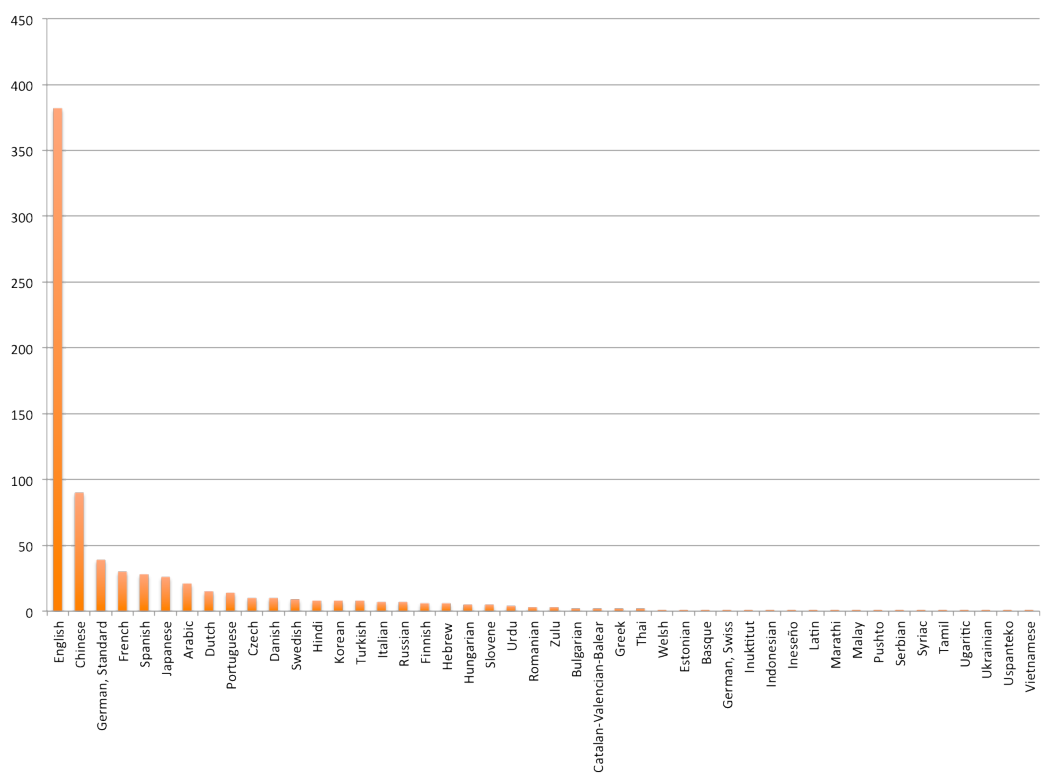
\includegraphics[width=0.75\textwidth]{../_media/Languages-in-LT-Research}
  \caption{Languages treated in research published in the 2010 edition of the Journal of Computational Linguistics and the conferences of ACL, EMNLP and COLING}
  \label{fig:languages-in-research}
  \colorrule{grey3}{\textwidth}{1.5pt}
\end{figure*}

Research activities have tended to be isolated, delivering valuable results but failing to make a decisive impact on the market. Even worse, in many cases research funded in Europe eventually bore fruit outside Europe. Google and Apple have been noteworthy beneficiaries. In fact, many of the predominant actors in the field today are privately-owned for-profit enterprises based in North America.

Most of their language technology systems rely on imprecise statistical approaches that do not make use of deeper linguistic methods and knowledge. For example, sentences are often automatically translated by comparing each new sentence against thousands of sentences previously translated by humans. The quality of the output largely depends on the size and quality of the available data. While the automatic translation of simple sentences in languages with sufficient amounts of available textual data can achieve useful results, shallow statistical methods are doomed to fail in the case of languages with a much smaller body of sample data or in the case of new sentences with complex structures. Analysing the deeper structural properties of languages is the only way forward if we want to build applications that perform well across the entire range of European languages.

Europe now has a well-developed research base. Through initiatives like CLARIN and META-NET the research community is well-connected and engaged in a long term agenda that aims gradually to strengthen language technology's role. Yet at the same time, our position is worse compared to other multilingual societies. Despite fewer financial resources, countries like India (22 official languages) and South Africa (11 official languages) have set up long-term national programmes for language research and technology development.

What is missing in Europe is a lack of awareness and of political determination and courage that would take us to a leading position in this technology area through a concerted funding effort, a major dedicated push.

Drawing on the insights gained so far, today’s hybrid language technology mixing deep processing with statistical methods should be able to bridge the gap between all European languages and beyond. In the end, high-quality language technology will be a must for all of Europe's languages for supporting the political and economic unity through cultural diversity.

Language technology can help tear down existing barriers and build bridges between Europe’s languages. In the digital age, communication with people and machines, as well as the unrestricted access to the knowledge of the world should be possible for all languages.

% FIXME: The following paragraphs are taken from the Executive Summary

The European LT community is dedicated to fulfilling the technology demands of the multilingual European society and to turn these needs and the emerging business opportunities into competitive advantages for our economy. To this end, we have developed this Strategic Research Agenda based on a shared vision and careful planning involving the major stakeholder communities.

In the first chapters we analyse the multilingual technology needs arising from the multicultural setup of our continent with its emerging single digital market. We also discuss the current state of technologies for European languages and the situation of the provider industries. The two core chapters of this document summarize our shared vision of the role of language technology in the year 2020 in non-technical terms (Chapter~\ref{sec:lt2020}, p.~\pageref{sec:lt2020}\,ff.) and outline three priority themes for large-scale research and innovation (Chapter~\ref{sec:pts}, p.~\pageref{sec:pts}\,ff.):

\begin{enumerate}
\item \textbf{Translation Cloud} -- Services for instantaneous reliable spoken and written translation among all European and major non-European languages
\item \textbf{Social Intelligence and e-Participation} -- understanding and dialogue within and across communities of citizens, customers, clients, consumers
\item \textbf{Socially Aware Interactive Assistants} -- analysis and synthesis of non-verbal, speech and semantic signals
\end{enumerate}
 
These thematic directions have been designed with the aim of turning the joint vision into reality and to letting Europe benefit from a technological revolution that will overcome barriers of understanding between people of different languages, between people and technology and between people and the accumulated knowledge of mankind.

The three research priority themes build the bridge between societal needs, LT applications, and concrete roadmaps for the organization of research, development and scientific innovation. The priority themes are contextualized in the advanced networked society and cover the main functions of language: storing, sharing and using of information and knowledge, as well as improving social interaction among humans and enabling social interaction between humans and technology. As multilingualism is at the core of European culture and becoming a global norm, one theme is devoted to overcoming language barriers.

We also present ways in which research and innovation need to be organized, in order to achieve the targeted breakthroughs and to benefit from the immense economic opportunities they create. Core components of the sketched strategy are novel modes of large-scale collective research and interaction among the major stakeholder constituencies: research in several disciplines, technology providers, technology users, policy makers and language communities. Effective schemes for sharing resources such as data, computational language models, and generic base technologies are also an integral part of the designed strategy. Of central importance is a rapid and effectual flow of intermediate results into profitable solutions of societal impact contributing to the fertile culture of technological, social and cultural innovation targeted by the Digital Agenda \cite{DA2010} and the programmes Connecting Europe Facility (CEF) \cite{CEF2011} and Horizon 2020 \cite{H2020}.

% This is a new paragraph (Georg)

The three research priority themes presented in this Strategic Research Agenda are mainly aimed at the programme Horizon 2020 which is foreseen to run from 2014 until 2020. The more infrastructural aspects, platform design and implementation and concrete language technology services are aimed at the programme Connecting Europe Facility. Our suggestion for integrating multilingual technologies into the wider CEF framework is to develop innovative solutions that enable providers of online services to offer their content and services in as many EU languages as possible, in a most cost effective way. These services are to include public services (e.\,g., eGovernment, eHealth, eCulture and open data portals), commercial services and user-generated content. An integral component of our strategic plans are the member states and associated countries: it is of utmost importance to set up, under the overall umbrella of our SRA and research priority themes, a coordinated initiative both on the national (member states, regions, associated countries) and international (EC/EU) level, including research centres as well as small, medium and large enterprises who work on or with language technologies. Only through close cooperation and tightly coordinated collaboration can we realise the ambituous plan of researching, designing, developing and putting into practice a European platform that supports all citizens of Europe and beyond by providing, among others, sophisticated services for communication across language barriers.

% FIXME: In Bezug auf die "Drei Kreise" Priority Themes Grafik und die Funding Programmes könnte man auch noch ein Bild malen: Die drei PTs sollen primär durch H2020 gefördert werden, die core technologies durch die Member States und auch H2020. Die European Platform hingegen soll primär durch CEF gefördert werden.

\end{multicols}

\clearpage

% --------------------------------------------------------------------------

\ssection[Multilingual Europe: Facts, Challenges, Opportunities]{Multilingual Europe:\newline Facts, Challenges, Opportunities}

\begin{multicols}{2}

\subsection{Europe's Languages in the Networked Society}
\label{sec:status-europes-languages}

Europe’s more than 80 languages are one of its richest and most important cultural assets, and a vital part of its unique social model \cite{EC2}. While languages such as English and Spanish are likely to thrive in the emerging digital marketplace, many European languages could become marginal in a networked society. This would weaken Europe’s global standing, and run counter to the goal of ensuring equal participation for every European citizen regardless of language. A recent UNESCO report on multilingualism states that languages are an essential medium for the enjoyment of fundamental rights, such as political expression, education and participation in society \cite{Unesco1}. From the very beginning, Europe had decided to keep its cultural and linguistic richness and diversity alive during the process of becoming an economic and political union. For maintaining the policy of multilingualism, the EU’s institutions spend about one billion Euros a year on translating texts and interpreting spoken communication. For all European economies the translation costs for compliance with the laws and regulations are much higher.

A single European market that secures wealth and social well-being is possible, but linguistic barriers still severely limit the free flow of goods, information and services. With the increased number of EU members and the general trend towards timely trans-border interaction, everyday communication between Europe’s citizens, within business and among politicians is more and more becoming confronted with language barriers. Many Europeans find it difficult to interact with online services and participate in the digital economy. According to a recent study, 57\% of internet users in Europe purchase goods and services in languages that are not their native language (English is the most common foreign language followed by French, German and Spanish). 55\% of users read content in a foreign language while only 35\% use another language to write e-mails or post comments on the web \cite{EC1}. A few years ago, English might have been the lingua franca of the web -- the vast majority of content on the web was in English -- but the situation has now drastically changed. The amount of online content in other European (as well as Asian and Middle Eastern) languages has exploded. Already today, more than 55\% of web-based content is not in English.

The fragmentation of languages on the web is highlighted by a study carried out by Google \cite{Ford11}. Figure~\ref{fig:language-graph-of-the-web} shows cross-lingual links excluding the English language, demonstrating that many European languages are practically isolated on the web.  Figure~\ref{fig:european-languages-in-twitter} shows the European language communities of Twitter: the map was created by identifying automatically the languages millions of tweets are written in and placing them onto a map using their GPS-coordinates \cite{fisher11}. To a large degree the resulting map replicates Europe's language borders -- and barriers.

\begin{figure*}[htb]
  \colorrule{grey3}{\textwidth}{1.5pt}
  \center
  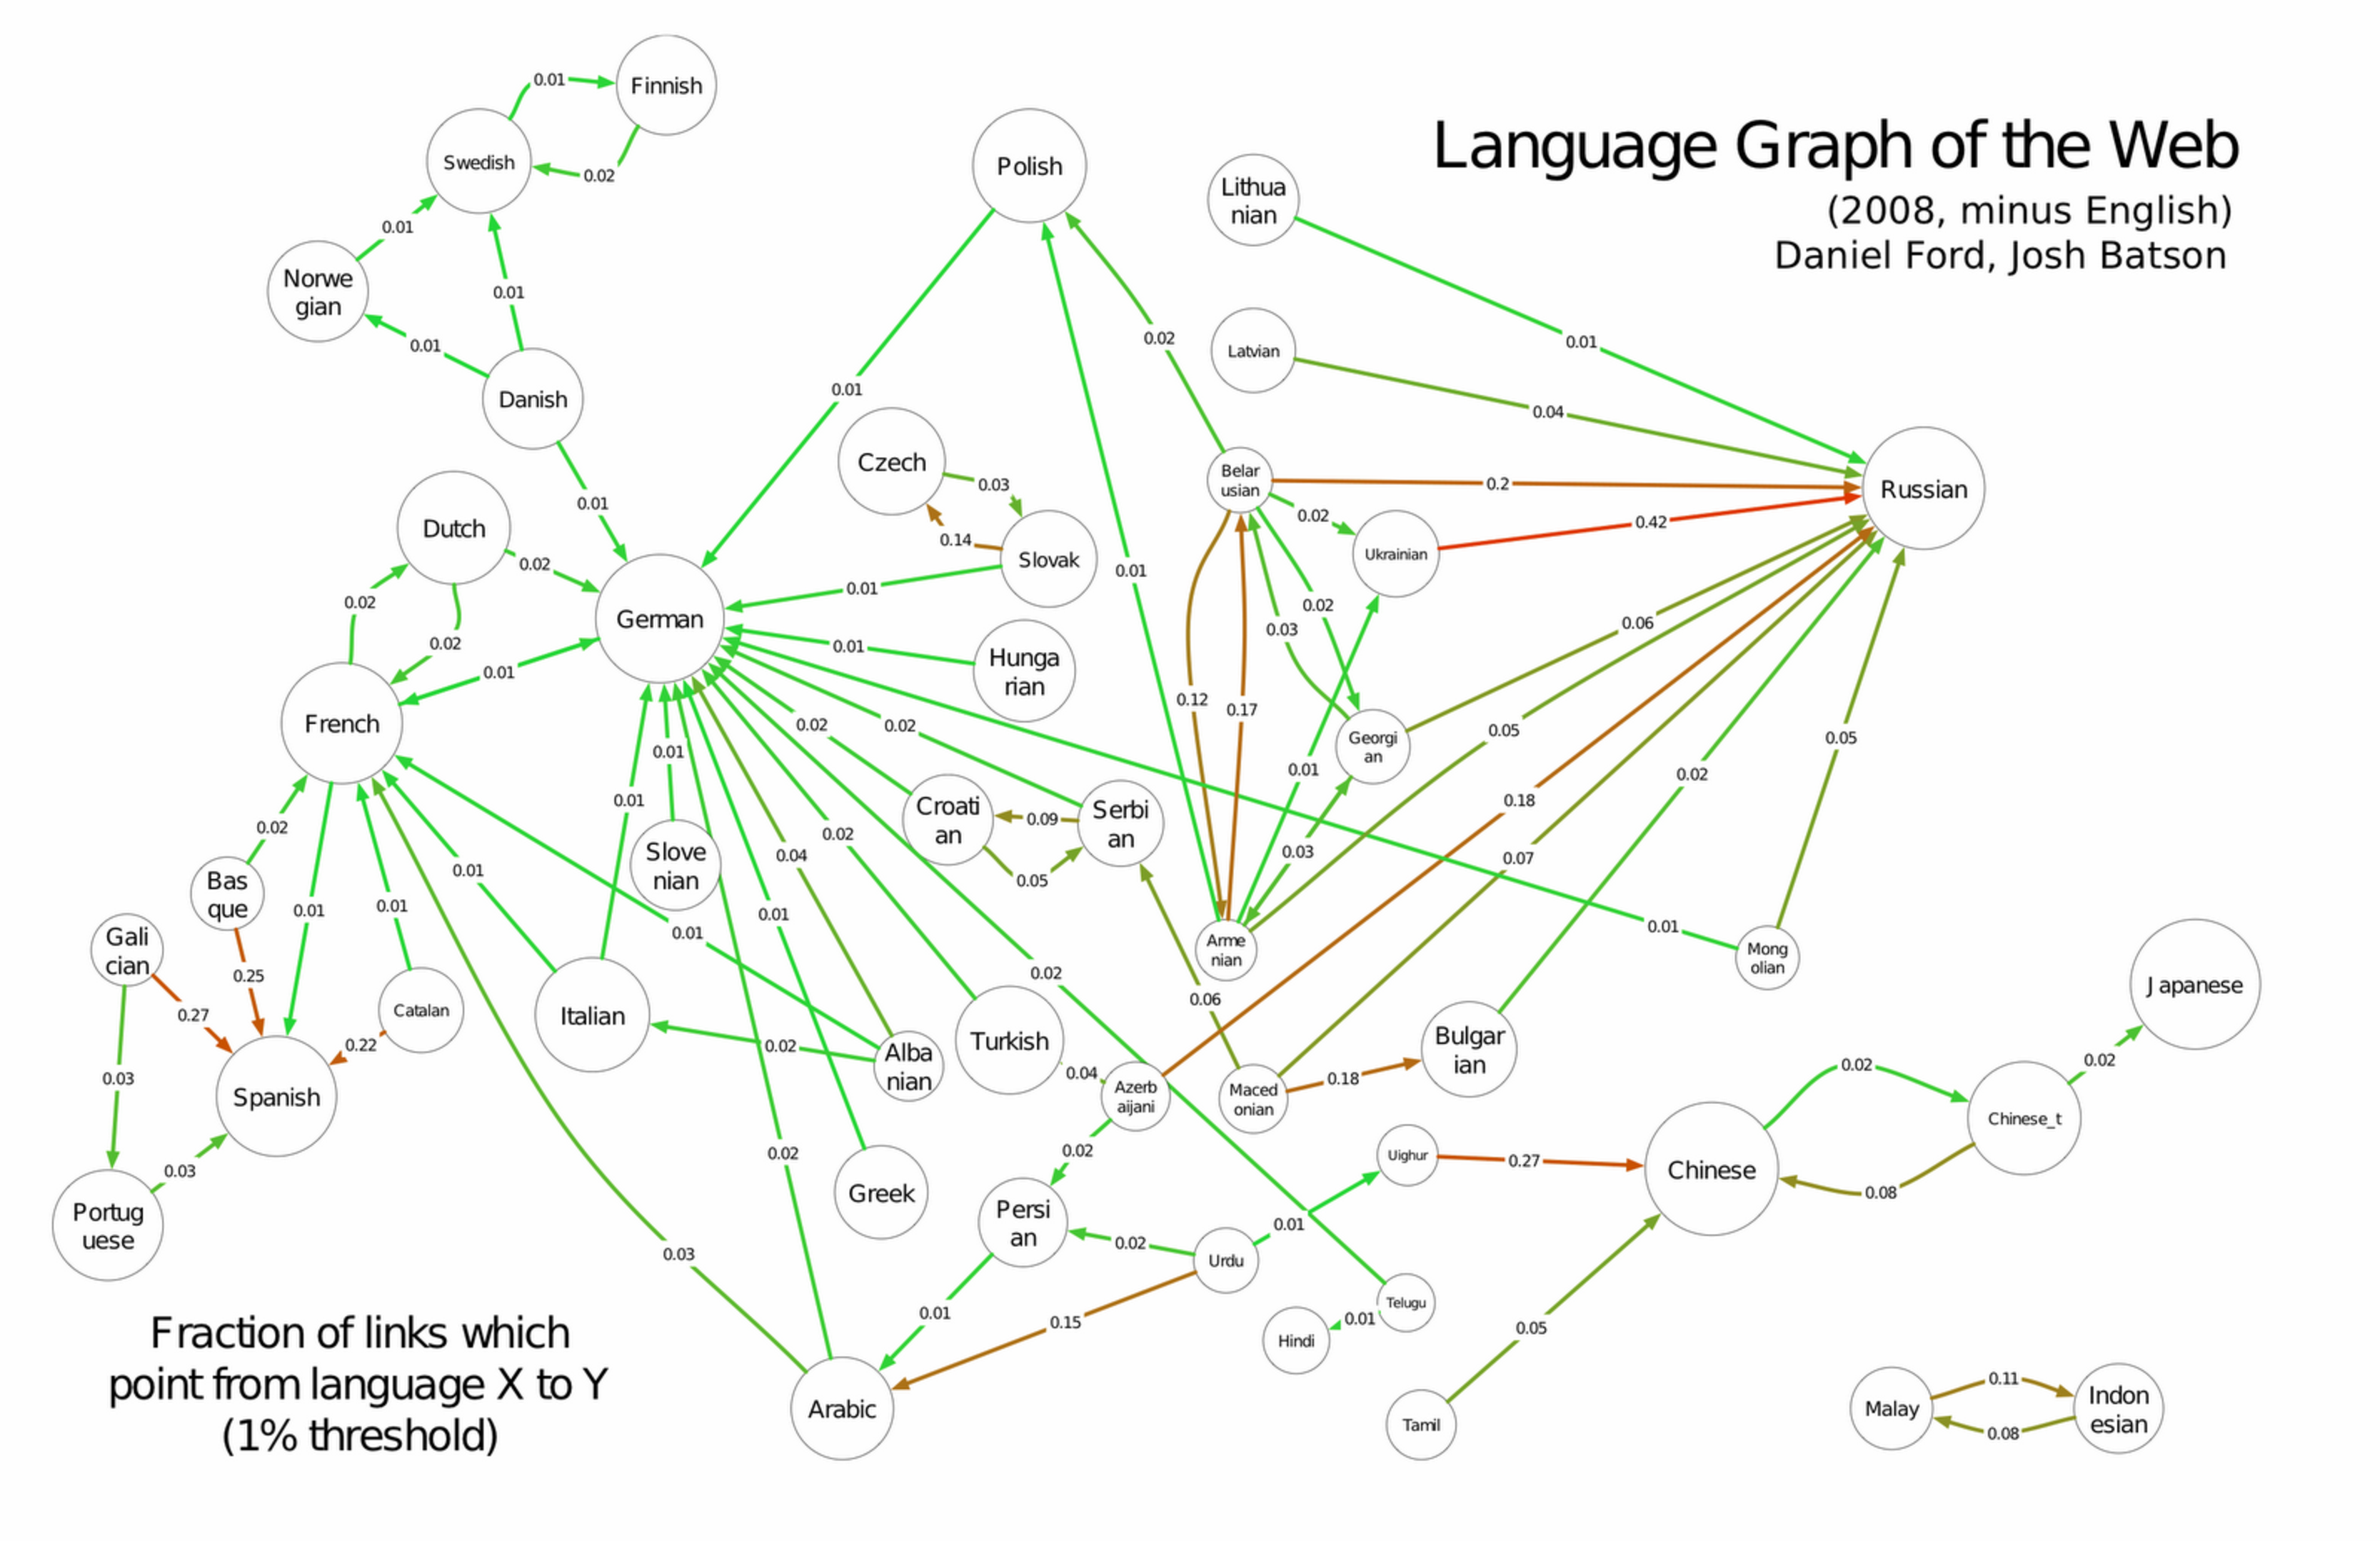
\includegraphics[width=0.9\textwidth]{../_media/Language-Graph}
  \caption{Language graph of the web}
  \label{fig:language-graph-of-the-web}
  \colorrule{grey3}{\textwidth}{1.5pt}
\end{figure*}

\begin{figure*}[htb]
  \colorrule{grey3}{\textwidth}{1.5pt}
  \center
  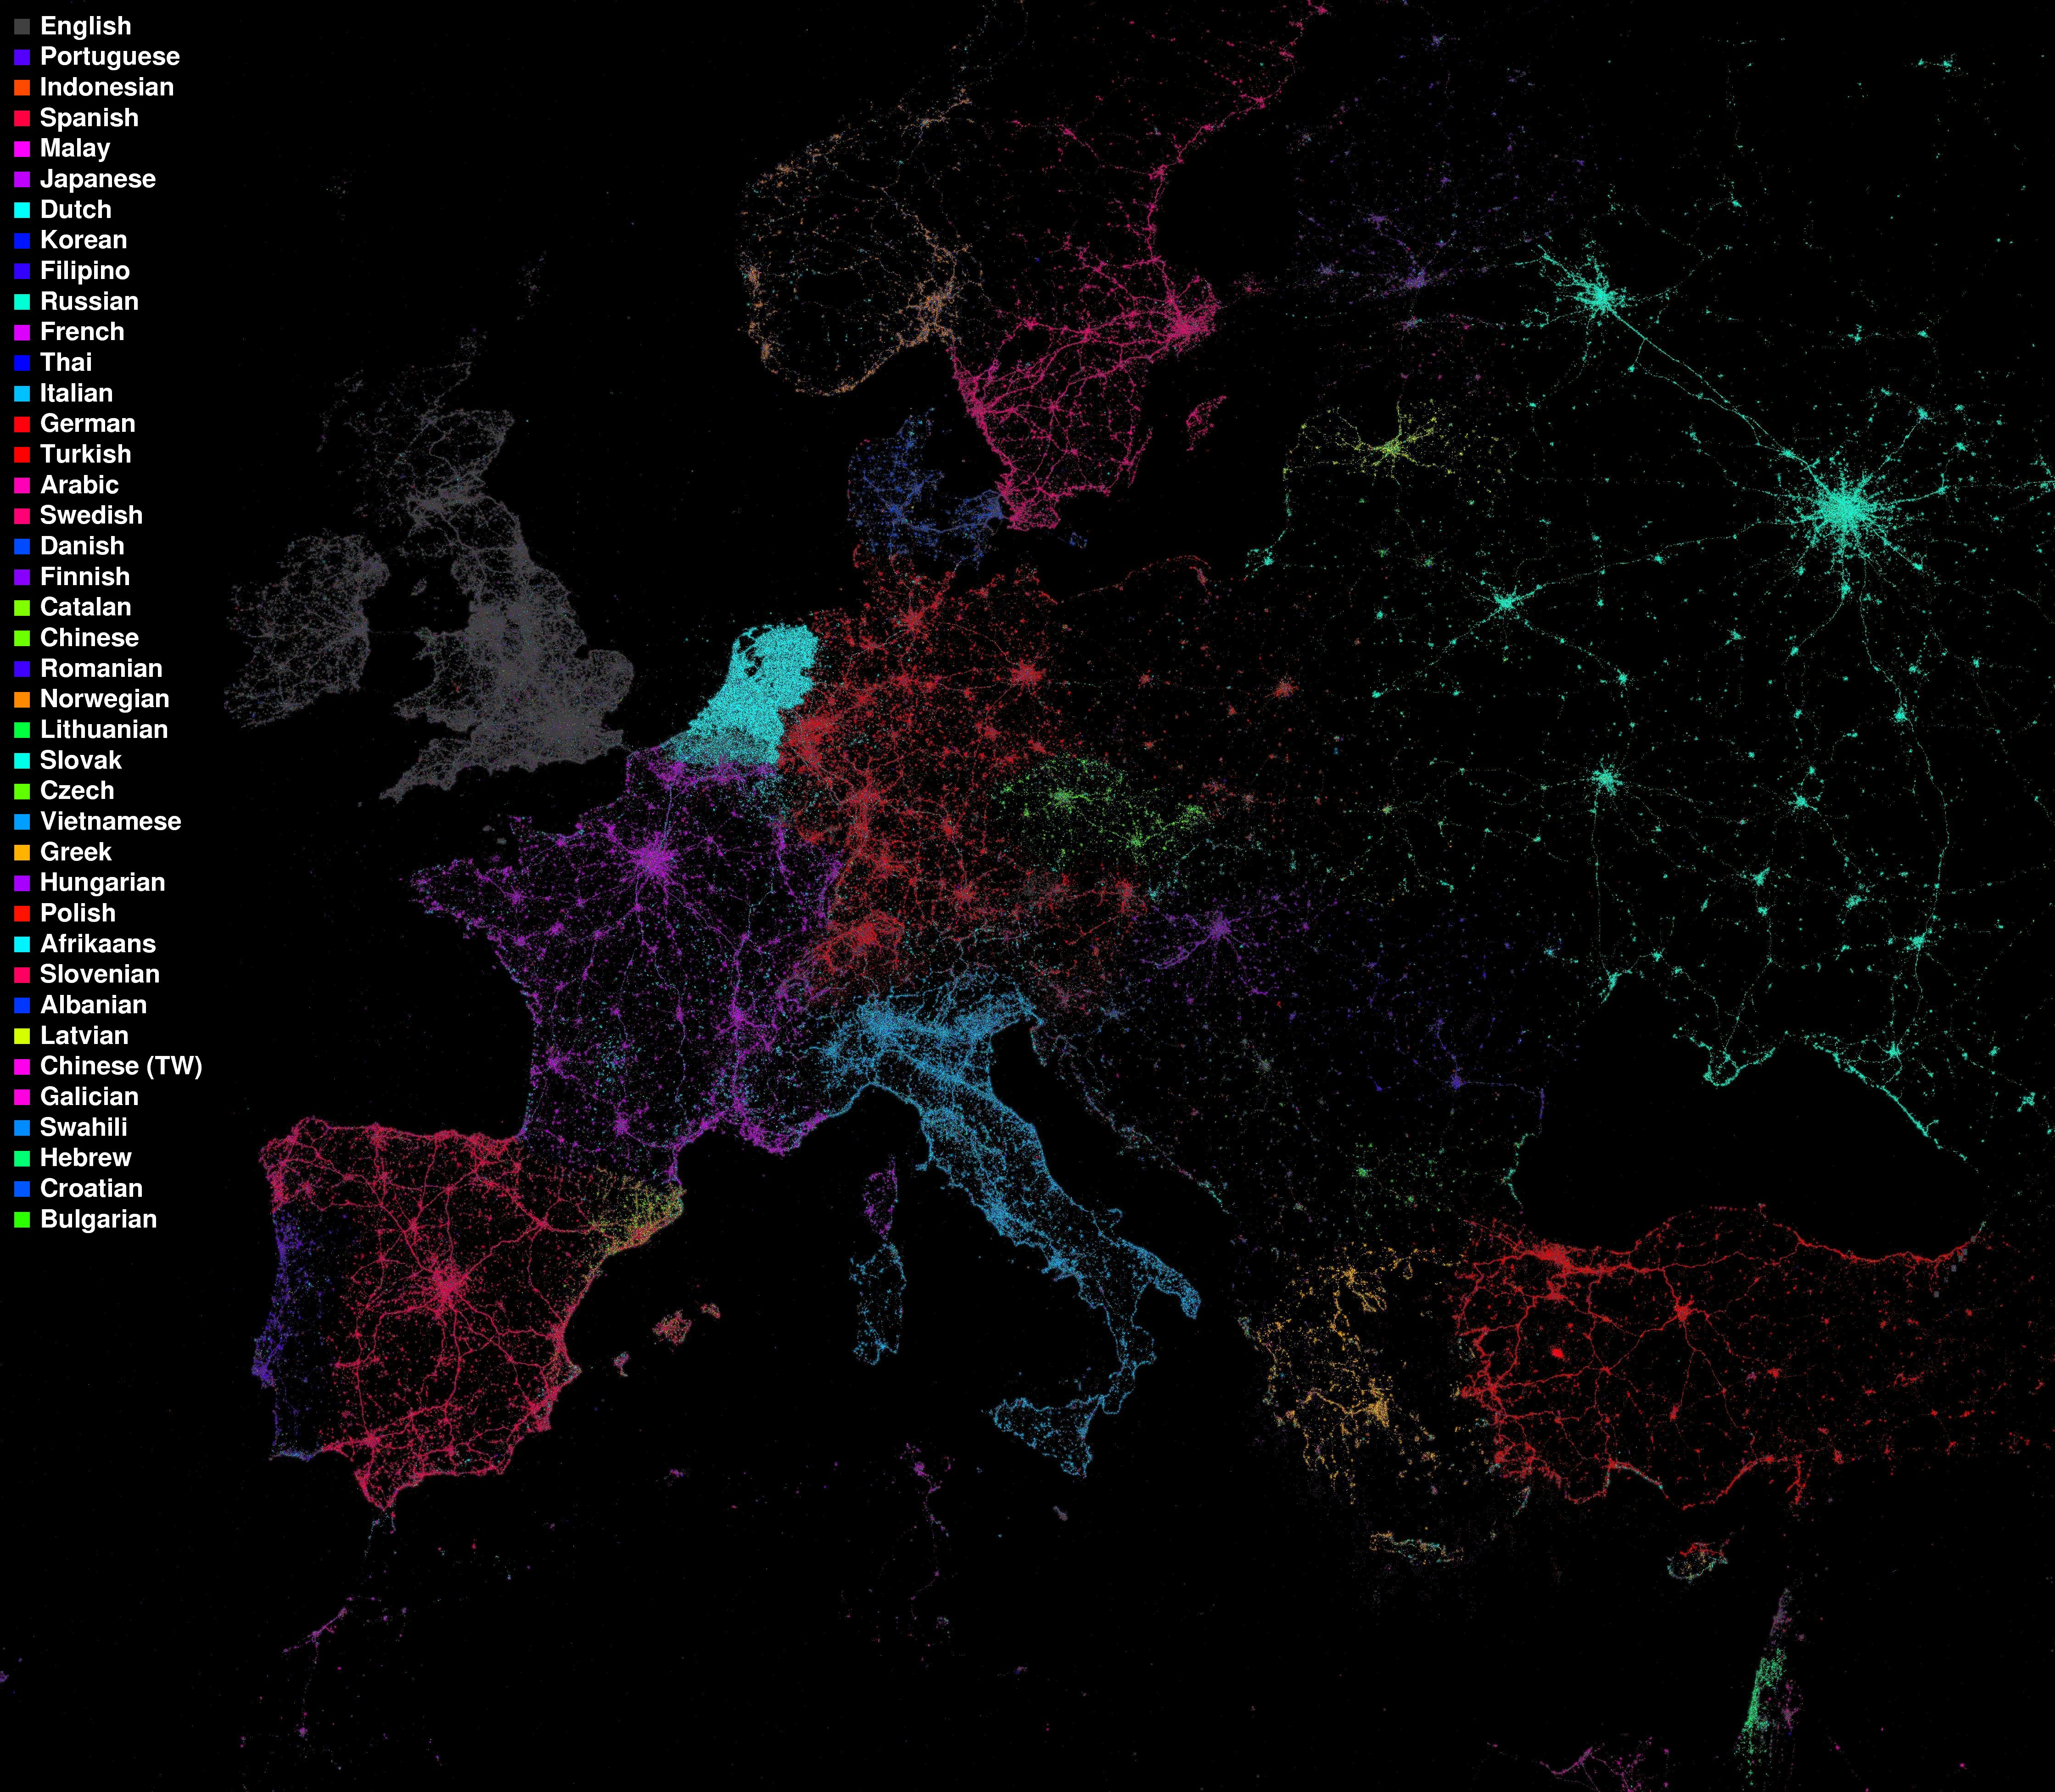
\includegraphics[width=0.9\textwidth]{../_media/twitter-languages-europe}
  \caption{Language communities of Twitter (European detail)}
  \label{fig:european-languages-in-twitter}
  \colorrule{grey3}{\textwidth}{1.5pt}
\end{figure*}

Surprisingly, this ubiquitous digital divide due to language borders and language barriers has not gained much public attention. Yet, it raises a very pressing question: Which European languages will thrive in the networked information society, and which are doomed to disappear?

The European market for translation, interpretation and localisation was estimated to be 5.7 billion Euros in 2008. The subtitling and dubbing sector was at 633 million Euros, language teaching at 1.6 billion Euros. The overall value of the European language industry was estimated at 8.4 billion Euros and expected to grow by 10\% per year \cite{EC3}. Yet, this existing capacity is not enough to satisfy current and future needs, e.\,g., with regard to translation. Already today, Google Translate translates about the same volume per day that all human translators on the planet translate in one year \cite{och12}.

Despite recent improvements, the quality, usability and integration of machine translation into other online services is far from what is needed. If we rely on existing technologies, automated translation and the ability to process a variety of content in a variety of languages -- a key requirement for the future internet -- will be impossible. The same applies to information services, document services, media industries, digital archives and language teaching. There is an urgent need for innovative technologies that help save costs while offering faster and better language services to the European citizen.

The most compelling solution for ensuring the breadth and depth of language usage in the Europe of tomorrow is to use appropriate technology. Still, despite recent improvements, the quality and usability of current technologies is far from what is needed. META-NET has conducted an analysis on the current state of the official EU languages as well as other important European languages with special emphasis on their language technology support. The result of this analysis is published in a series of white papers \cite{LWP2012} showing that, already today, especially the smaller European languages suffer severely from under-representation in the digital realm. Moreover, there are tremendous deficits in technology support and significant research gaps for all languages. For example, machine translation support for 23 out of the studied 30 languages was evaluated as having limited quality and performance, which is an alarming result! 

\subsection{How can Language Technology help?}
\label{sec:how-can-language-technology-help}

One way to overcome language barriers is to learn foreign languages. Yet without technological support, mastering the 23 official languages of the EU and some 60 other European languages is an insurmountable obstacle for Europe’s citizens, economy, political debate, and scientific progress. The solution is to build key enabling technologies: language technologies (LT) will offer all European stakeholders tremendous advantages, not only within the single market, but also in trade relations with non-European countries, especially emerging economies. Language technologies will eventually serve as the bridge between Europe’s languages.

Language technology is a key enabling technology for the knowledge society. LT supports humans in everyday tasks, such as writing e-mails, searching for information online or booking a flight. It is often used behind the scenes of other software applications. We benefit from language technology when we

\begin{itemize}
\item use spelling checkers in a word processor;
\item check product recommendations in an online shop;
\item hear the spoken instructions of a navigation system;
\item translate web pages with an online service. 
\end{itemize}

Several popular language technology services are provided by American companies, some of them free of charge. The recent success of Watson, an IBM computer system that won against human candidates in the game show Jeopardy, illustrates the immense potential of language technology. As Europeans, we urgently have to ask ourselves a few crucial questions:

\begin{itemize}
\item Can we afford our information, communication and knowledge infrastructure to be highly dependent upon monopolistic services provided by US companies?
\item What is Europe's fallback plan in case the language-related services provided by US companies that we rely upon are suddenly switched off?
\item Are we actively making an effort to compete in the global landscape for research and development in language technology?
\item Can we expect third parties from other continents to solve our translation and knowledge management problems in a way that suits our specific communicative, societal and cultural needs?
\item Can the European cultural background help shape the knowledge society by offering better, more secure, more precise, more innovative and more robust high-quality language technology?
\end{itemize}

We believe that \emph{Language Technology made in Europe} will significantly contribute to future European cross-border and cross-language communication, economic growth and social stability while establishing for Europe a worldwide, leading position in technology innovation, securing Europe's future as a world-wide trader and exporter of goods, services and information.

\subsection{Language Technology and Societal Challenges}
\label{sec:what-soci-challenges}

With regard to the future information society there is a strong likelihood that the revolution in communication technology will bring people speaking different languages together in new ways. This is putting pressure on individuals to learn new languages and especially on developers to create new technology applications. In a global economy and information space, more languages, speakers and content interact more quickly with new types of media. The current popularity of social media (Wikipedia, Facebook, Twitter, YouTube, Google+, Pinterest, Instagram etc.) is only the tip of the iceberg.

Many societal changes and economic trends confirm the urgent need to include sophisticated language technology in our European information and communication technology (ICT) infrastructure. Research, development and innovation efforts in LT must increase to go beyond what is possible today.

\textbf{Linguistic, Commercial and Knowledge Barriers.} A recent study on cross-border online commerce in the EU clearly indicates that language barriers are economic barriers \cite{EC4}. Only 59\% of retailers can handle transactions in more than one language. Translation and localisation costs must be drastically lowered before broad participation in Europe’s single digital market is a reality. Multilingual language technology is the key, especially for SMEs. At the same time, user expectations are increasing: 81\% of all internet users think that websites run in their country should also be available in other languages. 44\% of European users think they miss out on interesting information because websites are not available in a language they understand \cite{EC1}. These facts can no longer be ignored. The availability of reliable LT can help establish a potentially vast market for information as well as consumer and entertainment goods in any language.

\textbf{Ageing Population.} Demographic changes suggest the need for more assistive technologies, especially those that drastically improve spoken language access. An aging population requires technology that can help master everyday situations and provide proactive guidance. Such technologies could answer the question, “Where did I leave my glasses?” The economic cost of demographic changes will also mean that more health care services and support systems will be required in our homes. Ambient assisted living (AAL) technologies can greatly benefit from a personalised, spoken method of interaction that is possible due to recent developments in the field of dialogue systems and interactive assistants.

\textbf{People with Disabilities.} The way we deal with disabilities has changed dramatically in the last 20 years. It shifted from an approach based on assistance, recovery or maintenance of functional capabilities to the goal of full integration. New technologies can help us reach the ambitious goal of achieving equal opportunities and promoting independent living. Language technologies already help people with disabilities to participate in society. Noteworthy examples include screen readers, dictation systems and voice-activated services. In addition to the social aspect there is a huge commercial market for future technologies such as, for example, full dialogue systems and interactive assistants, sign language recognition and synthesis, automatic translation, summarisation and content simplification. Approximately 10\% of Europeans (50 million citizens) have permanent disabilities.

\textbf{Immigration and Integration.} According to the United Nations' International Migration Report 2002, 56 million migrants lived in Europe in 2000 \cite{UN1}. The number of migrants has grown roughly to 60 million people today. Facilitating communication, providing access to information in foreign languages and helping people learn European languages can help better integrate migrants into European society. In fact, speech and language technologies can dramatically improve the integration process by providing intelligent language learning environments, automatic subtitling services in real time and automatic translation services.

\textbf{Personal Information Services and Customer Care.} Broadband access to information and services is common, mobile communication is daily routine for millions of Europeans. In this 24/7 economy we expect quick and reliable answers as well as engaging and timely online news broadcasts. However, information overload is also common, and it limits exchange in the digital information society. Citizens, governments and industries would greatly benefit from new technologies that help get the situation under control again. Embedded mobile applications enhanced with language technology will become personal assistants to everyone, offering automatic and intelligent question answering and dialogue capabilities, as well as automatic, personalised and trusted text and speech processing of messages, news items and other content.

\textbf{Global Cooperation and Human Communication.} Companies need to address new markets where multiple languages are spoken and support multinational teams at multiple locations. Many jobs cannot be filled today because linguistic barriers exclude otherwise qualified personnel. A flexible and mobile population requires multilingual language skills. Improvements in language technology can enable richer interactions and provide more advanced video conferencing services. Future technologies like a three dimensional internet can enable new modes of situation-based collaboration in the workplace as well as support more realistic training and education scenarios. We will soon be able to participate in virtual events as new forms of entertainment, cultural exchange and tourism. Combining 3D virtual worlds and simulations with multilingual language technology including simultaneous translation, automatic minute taking, video indexing and video searching will let us experience being European in a brand new way.

\textbf{Preservation of Cultural Heritage and Linguistic Diversity.} According to the principles of the UN-endorsed World Summit on the Information Society \cite{worldsummit2003}, the “Information Society should be founded on and stimulate respect for cultural identity, cultural and linguistic diversity.” Much effort has been put into the creation of digital archives and virtual museums that should help promote our cultural heritage. However, digitisation and digital asset management are only the first step. The amount of available information and language barriers still hinder the enjoyment and usage of our cultural treasures. Language technology can make this content accessible, e.\,g., through cross-lingual and multimedia search and machine translation. Likewise, communication skills need to be trained, especially in the light of today’s find-remix-share paradigm of social media. This is underlined by the UNESCO Information for All Programme \cite{Unesco2}, which seeks to “support the production of local content and foster the availability of indigenous knowledge through basic literacy and ICT literacy training.” Computer assisted language learning and language technology should be embedded into didactic software and games to help rescue our linguistic knowledge and diversity.

\textbf{Social Media and e-Participation.} Participation in online social media is a key characteristic of the early twenty-first century. Social media have a tremendous impact on practically all areas of society and life. Social media can help us solve technical problems, research products, learn about interesting places or discover new recipes. At the same time, recent developments in North Africa demonstrate the ability of social media to bring citizens together to express political power. Social media will play a role in the discussion of important, future topics for Europe like a common energy strategy and a common foreign policy.  A severe problem is that certain groups are becoming detached from these developments. One can even speak of a broken link regarding communication cultures. This is an issue since both types of bottom-up movements sketched above are highly relevant for politicians, marketing experts, and journalists who would like to know what their customers or citizens think about their initiatives, products, or publications and to be able to react accordingly. However, it is not possible to process manually the sheer amount of information generated in multiple languages on social networks. We need to develop sophisticated language technology that is able to analyse these developments in real time.

\textbf{Market Awareness and Customer Acceptance.} Language technology is a key part of business and consumer software. The exact size of this market is difficult to assess because LT is often hidden inside other, more visible products. Customer acceptance of LT has recently been shown to be high. For example, market research by the Ford Motor Company indicates that their voice control system, Ford SYNC, is widely accepted \cite{ford}. 60\% of Ford vehicle owners use voice commands in their cars. Non-Ford owners report a three-fold increase in their willingness to consider Ford models while 32\% of existing customers admit that the technology played an important or critical role in their purchase decision. Language technology has a tremendous market potential.

\textbf{One Market, Many Languages.} Support for the 23 official languages of the EU has major economic and social implications, but the political dimension is equally important. Europe currently lags behind countries such as India (22 “official” languages) and South Africa (11 national languages). Government programmes in these two countries actively foster the development of language technology for a significant number of official languages (India: \url{http://tdil.mit.gov.in}; South Africa: \url{http://www.meraka.org.za/nhn}). Mobile devices will become an even more important connection point between humans and information technology. Google already provides free translation services in 3,306 different language pairs as well as voice input for 16 languages and speech output for 24 languages. Apple's App and iTunes Store has demonstrated how premium content and products can be marketed for free and for a fee. Europe must address this global competition.

\textbf{Secure Europe.} The evolving information and knowledge society has improved human communication and information access, but the same communication networks also help some to commit crimes such as identity theft and internet fraud. The effective persecution of illegal activities requires automatic tools that can help detect crimes and monitor offenders. Language technology can help to build systems that can monitor, analyse and summarise large amounts of text, audio and video data in different languages (European and non-European) and from different sources (websites and social media).

The solutions presented above are strongly influenced by larger trends (see the following chapter), such as cloud computing, social media, mobile apps and web services. Many of these products and services are only available online. For example, severely restricting access to Facebook and Twitter strongly influenced recent political developments in North Africa. In Europe, the idea of social innovation has recently gained interest as it “offers an effective approach to respond to social challenges by mobilizing people's creativity to develop solutions and make a better use of scarce resources” \cite{EC5}. Social innovation, which is also part of Europe’s 2020 strategy, critically relies on active involvement of citizens and interaction among them, which calls for supportive multilingual language technologies.

Multilingualism has become a global norm rather than an exception. Future 3D applications that embed information and communication technology require sophisticated language technologies. Fully speech-enabled autonomous robots could help in disaster areas by rescuing travellers from public transportation or by giving first aid. Language technology can significantly contribute towards improving social inclusion. Language technology can also help us provide answers to urgent social challenges while creating genuine business opportunities.

Language technology can now automate the very processes of translation, content production, and knowledge management for all European languages. It can also empower intuitive language/speech-based interfaces for household electronics, machinery, vehicles, computers and robots. Real-world commercial and industrial applications are still in the early stages of development, yet R\&D achievements are creating a genuine window of opportunity. For example, machine translation is already reasonably accurate in specific domains, and experimental applications provide multilingual information and knowledge management as well as content production in many European languages. 

\subsection{Market Opportunities}
\label{sec:market-opportunities}

There is an immensely large set of interesting and promising market opportunities around Language Technologies in Europe. Instead of duplicating efforts and work, we agreed with the EC-funded initiative ``LT Innovate'' (``LT-Innovate is the Forum for Europe's Language Technology Industry'', see \url{http://lt-innovate.eu}) that we will include a concise description of the market opportunities into this document once their ``LT Innovation Agenda'' has been prepared.

\end{multicols}

\clearpage

% --------------------------------------------------------------------------

\ssection[Major Trends in Information and Communication Technologies]{Major Trends in Information and Communication Technologies}

\begin{multicols}{2}

\subsection{The Current State}
\label{sec:ict-trends}

Networked computers are ubiquitous. They come in many different shapes and forms (desktop, laptop, mobiles, tablets, etc.) or are embedded in devices, objects, and systems (e.\,g., smartphones, cameras, washing machines, cars, heating systems, robots, factories, traffic control systems). Software is usually available in multiple languages. Standardisation efforts such as the introduction of Unicode solved the problem of representing and displaying different scripts, alphabets and special characters. The main use cases for today's computers are text processing, spreadsheets, presentations, communication (e-mail, Facebook, Twitter, Skype etc.) and entertainment (photos, music, films, games).

Mobile devices and social media are ever more reshaping how and when we communicate with one another using the tools and devices we use both in business and private life. The way we interact with computers is no longer restricted to graphical user interfaces with limited functionality but it is being extended through touch screens, voice interfaces and dialogue systems, tactile interfaces and mobile devices with built-in accelerometers that tell the device how it is held by the user.

Language technology is currently not well integrated into applications and interfaces -- to the end user, spelling and grammar checking seem to be the only notable exception. A trend towards more intelligent language-based interaction is illustrated by Apple’s introduction of the mobile assistant Siri in the latest iPhone.

The web represents much of our knowledge. It emerged as a collection of static documents. Nowadays it is first and foremost a collection of systems and databases that can be queried through APIs, and applications such as Google Mail, Google Calendar, Facebook, eBay and Amazon. Many people only need one interface application on their computers: a web browser. Others use netbooks whose operating system more or less \emph{is} the browser (Chromium OS). Behind the scenes, there is already a considerable amount of language technology incorporated in web applications such as search engines, dialogue systems, or machine translation services.

% =========================================================================================

\subsection{Hardware}
\label{sec:hardware}

Networked computers are no longer as big as a refrigerator, the age of the clumsy tower or desktop computer is over. Nowadays, networked computers come in many shapes and forms: small mobile devices (smartphones using, for example, the Android or iOS operating system), tablets, netbooks, ultra-portable and very lightweight laptops, small desktop computers, ebook readers, radios, television sets, gaming consoles and other entertainment devices with built-in wireless and access to, for example, RSS feeds, internet radio stations or youtube, cameras or house-hold appliances such as vacuum cleaners, coffee machines or scales that push the weight of the user to the cloud from where it can be monitored using an app on the smartphone. The next revolution in the hardware market will be wearable computers. Google has already demonstrated a prototype of their Google Glasses product in which the computer visuals are projected into a head-up display that looks like a regular pair of glasses. This approach can be used to provide the user with a true augmented reality perspective and a hands-free computing environment which immediately brings up the question if it will be possible to interact with the Glasses, or a similar product, using only your voice.

The shape and size of computers is no longer determined by the shape and size of their internal hardware components. Due to further breakthroughs in miniaturisation, the form of computers now truly follows their function. While computers and devices with embedded systems get smaller and smaller, the distributed data centres around the world get bigger and bigger -- both in terms of number and size. The concept of cloud computing and storing data in dedicated data centres from where the data can be accessed by multiple devices (see, for example, Apple's iCloud), is already mainstream and used by millions of consumers world-wide. An important reason for the success of using the cloud to store data is the fact that, by now, people tend to have more than one computer, a not too unusual setup may include a laptop, a smartphone, a tablet and another computer as a dedicated media centre. Cloud services are ideal for synchronising data between all devices without buying, configuring and administering your own server machine.

% ========================================================================================= 

\subsection{Software}
\label{sec:software}

The trends in the software area are much more multi-dimensional -- in this section we can only scratch the surface and highlight several recent developments and current trends.

\textbf{Communication:} Probably the most important cornerstone of today's computer use is communication (both human to human and human to machine), be it more direct communication via traditional e-mail, instant messaging, text-based chat systems, video chat between two people or larger groups (Skype, Facetime, Google Hangout) or indirect communication and staying in touch with friends, acquaintances and colleagues via social networks such as Twitter, Facebook, XING and LinkedIn or social media such as blogs, YouTube, Pinterest or Instagram. An important factor is that millions of people world-wide are, by now, always online using several different networked devices including their phones. 

\textbf{Search and Information Services:} Another important use case of any type of computing device is to search for information and to make use of specialised information services. Important applications are web search engines such as Google Search or Microsoft's Bing, Wikipedia, Google News, Google Books, digital libraries such as Europeana, meta-search engines and RSS feed aggregators etc.

\textbf{Location-based Services:} Search queries are nowadays often coupled to the user's current location. Location-based services enable the user to search for certain information in his or her geographic area, to make use of online maps, navigation systems, recommender systems such as Yelp or Qype or to find tweets or photos on Instagram in his or her geographic area.

\textbf{E-Commerce and Shopping:} World-wide billions of Euros are spent each year using general online shops such as Amazon or eBay or shops run by specific brands or services, reservation and booking, online banking and brokering services etc. 

\textbf{Media and Entertainment:} Different types of media (photos, videos, music, sounds, text and multimedia documents, audio and video podcasts, ebooks, films, tv programmes etc.) play an important role. Not only personal media and other user-generated content are often connected to social networks (posting photos or videos on Instagram, Facebook, Google+, Flickr or YouTube), songs, photos or videos created and posted by third parties are also often shared using social networks. Almost all of the media mentioned above can be purchased using general or specific online stores, for consumption on any device. Another important category of software is games, from online Flash games to games that are embedded into social networks, location-based games, multi-player games with millions of users to very simple but also very successful casual games such as Angry Birds.

\textbf{App and Media Stores:} The success of ecommerce platforms, online shopping and the increased use of digital media led to the development of dedicated app and media stores. By now it is possible to buy or to rent almost every movie ever made (Amazon, iTunes), to buy music (iTunes music store), to stream music from the cloud onto your device (Spotify) and to buy software and mobile apps through dedicated stores (e.\,g., Apple's app stores for MacOS and iOS) without any need to ship physical media. An important development is in-app purchasing, especially on mobile devices: with a single tap of a finger it is possible to buy, within a specific app (which is usually available for free), additional modules, components or data sets for a small price.

\textbf{Personal Information Management:} With the ever increasing number of personal and professional contacts (including social networks), meetings and personal errands to run, there is a big trend towards personal information management. This includes address and contacts databases that are often integrated into larger applications such as Google Contacts (embedded in, among others, Google Mail) or Apple's AddressBook (used in Apple Mail). Cloud-integration is an important feature, so that contact information (including names, email address, phone numbers, photos etc.), calendar entries, ``to do'' items and the data from other productivity tools are always available on all devices. 

\textbf{Office Applications:} The classic office applications --~word processors, spreadsheets, presentations~-- are still important in the professional context and also in home use. Nowadays, there are several applications to choose from including open source software, cloud-based services and applications for Apple's iOS (MS Office, Apple iWork, Open Office, Google Docs). Except for Open Office all office suites use the cloud to enable the user to, for example, finish work on a presentation at the desktop computer where the document is automatically pushed to the cloud and to continue working on the presentation on a mobile device on the way home.

To sum up, one of the most basic common denominators of all pieces of software is language -- language plays a central and integral part in practically every single app, tool or application. Ironically, however, language technology as such (including text analysis, information retrieval and extraction, spelling and grammar checking, speech recognition and synthesis, dialogue systems etc.)~is usually completely hidden from the user, integrated into bigger applications, working behind the scenes. There is, however, a clear trend to embed language technologies not only at the level of the single application but on the level of the operating system (see, for example, the speech synthesis engine built into MacOS or the speech recognition and synthesis capabilities of iOS~5 with Siri). Another important factor of current computing is communicating and interacting with other people or groups of people, both on the personal level and also for business purposes.  A third crucial ingredient of computing today is information, especially structured information which is annotated based on specific standards (see, for example, the family of standards around XML, Semantic Web, Linked Open Data, Web Services etc.).

\subsection{Current Trends and Mega-Trends}
\label{sec:major-trends}

In the following we briefly sketch the current trends and mega-trends, loosely grouped into three sections.

\textbf{Internet:} The internet will continue to be \emph{the} main driving force behind future developments in information and communication technologies. There are several mega-trends tightly coupled to the internet and network technologies: among these are cloud computing and cloud services, including cloud storage, as well as linked open data and the semantic web. Social media and social networks will continue to change everything and to penetrate the market further, including niche markets, driven by location-based services. With the predominance of social networks we expect a certain convergence of digital identities that will enable users to have and to maintain one central digital identity that feeds into their multiple social network profiles including also a merger of the business-self and the private-self. Along those lines, exchanging and distributing personal data and information (photos, videos, music etc.) in a secure way will become easier. We further expect more broad deployment and general acceptance of services in the areas e-democracy and e-government (including open data portals) and a continued increase of e-commerce platforms and services. A perceived general information overload will continue to be a problem, although modern search engines, aggregation services and user interfaces help a lot; web search is generally considered a solved problem. New business models and ways to distribute content or services to the end-user will continue to emerge (see the different app stores and approaches such as in-app purchases).

\textbf{People:} Information and communication technologies are used by people -- the predominance of social networks and being always-on using smartphones, tables and laptops, are responsible for the fact that the way people interact, communicate and do business with one another will continue to be redefined and reshaped completely, including novel approaches for participation and public deliberation processes. Communication tools such as email, Twitter, Facebook etc.~are mainstream by now and used across all age groups. This trend will continue. A popular phrase that characterises the main essence of the success factor of social networks is ``faces and places'' as this is what people are mainly interested in: other people first and foremost as well as certain buildings, restaurants, cinemas, landmarks and many others. The trend to use location-based services to find current friends, items of interest or even new friends with similar interests on social networks will continue (along with a more in-depth discussion of privacy issues). We also expect a tighter connection between the data stored in social networks and the linked open data cloud as well as a tighter connection between tools for personal information management and linked open data.

\textbf{Hardware and Software:} By now many internet companies operate under the slogan ``mobile first''. Accessing the internet or using web services on mobile devices will overtake the use of desktops and laptops very soon. There is also a clear tendency for completely novel mobile devices with Apple's iPad and Google's Glasses being two prime examples; in addition, there is a tendency for more household-appliances connected to the internet (tv, radio, gaming consoles, refrigerator, scales, coffee machine, lamps etc.; see the Internet of Things). Many of these devices will not have any displays but voice-driven interfaces. We expect a seamless integration of mobile devices into the hardware landscape at home including very simple file, data and application transfer and exchange among arbitrary mobile or stationary devices, playing music or movies on arbitrary displays or video projectors etc. Very soon there will not be a need anymore for the average user to own a laptop or desktop computer because mobile devices (phones and tablets) will cover all basic needs. As regards networks, their capacity and bandwidth will continue to grow, mobile telecommunication networks will gradually become more important than, for example, ADSL lines. The quality of voice or video calls (Skype, Facetime, Google Hangout) will continue to improve, phones and all other devices will continue to become faster, have more storage as well as 3D-capable displays that offer more intricate modes of interacting with the device. Mobile phones will have built-in facilities to replace credit cards for payment purposes (for example, using Near Field Communication), effectively replacing the wallet. Finally, the market for apps, especially mobile apps, will continue to grow. Nowadays many companies, services and events have their own app that users can interact with and that usually offer added value when compared to the respective website. In order to be successful on the app market, usability will continue to be a decisive factor: only those apps will be successful that users can interact with intuitively right away.

To sum up, information and communication technologies will continue to be ubiquitous, available wherever and whenever needed. These technologies will be services that combine widely distributed applications, resources and data. They will be able to adapt to the location, situation and needs of the user including current emotions, habits and goals. As can be seen by the success of Wikipedia and other collaboratively edited knowledge bases, it is only a matter of time until a gigantic digital model of our world will exist that consists of interlinked and overlapping components. Naturally, languages and especially the automatic processing of languages using sophisticated language technologies will play a key role in this development. Now is the time to realise the needed breakthroughs. High performance, robust machine translation and related language technology services are urgently needed. There is a huge window of opportunity for consumer-oriented language technology: mobile devices are fast enough and have enough computing power, memory and a direct internet connection; they have a camera and are always online; it is easy to buy apps or add-ons.

While the LT-related aspects will be further discussed in the following chapters, we provide a more in-depth discussion of two selected trends in sections~\ref{sec:linked-data-open} and~\ref{sec:cloud-sky-computing}.

\subsection[Selected Trend: Linked Open Data]{Selected Trend:\newline Linked Open Data}
\label{sec:linked-data-open}

Data is considered one of the main topics of the future. At the European Data Forum 2012 and several other occasions the ``data challenge'' (big data, open data, linked data and the data value chain) is seen as one of the main themes and driving forces for future developments in information technology. Language technology and the priority research themes described later have strong relations to the data challenge, both as contributors and as beneficiaries. On the one hand, LT can help to exploit the immense volumes of information, knowledge and data encoded through natural language in text documents. LT can extract information from texts and make them accessible as structured data for automatic processing. On the other hand, LT will be able to analyse and interpret language data much better if it can use the growing volume of available structured data as background knowledge. 
%
Most of humankind's knowledge, reflection, communication and planning is encoded in and through human language. Conceptualising language as an integral part of the growing data universe is the ultimate challenge for the “big data movement”. Interpreting and interlinking textual knowledge with the linked data world will help in the process of extracting new knowledge from the masses of newly produced structured data.

The Translation Cloud will benefit from data available across languages. The translation technologies being developed will also help to address data challenges, like building and cleaning data sets that span across languages or building links between existing data sets within one or between several languages. Multilingual access is an important requirement for a European vision of eGovernment and eParticipation services. On the one hand, language technology can make use of open, governmental data that is being developed in portals like data.gov.uk or within the upcoming European data portal. On the other, improving language technologies is inevitable for realizing multilingual access to public sector data for all European citizens: the sheer amount of data and language barriers between data sets are obstacles that can only be removed with technologies in the realm of, e.\,g., machine translation, cross-lingual information access and information extraction. Finally, one application scenario of Socially-Aware Interactive Assistants are multilingual virtual meetings that make use of shared data sets that provide information about individuals, organizations and interactions settings. The creation of these data sets is a challenge in terms of privacy and re-use of data. This leads to various open issues that need to be resolved both for the data challenge in general and for language technologies:

\begin{itemize}
\item Is there a need for a public data infrastructure versus a private infrastructure, having implications with regards to data re-use, licensing schemes, privacy etc.?
\item Provenance and origin information of data sets with regard to trustworthiness, data quality, privacy and re-use aspects need to be provided as part of the whole data value chain.
\item In the realm of LT and localization, a huge amount of data has been developed that is crucial for processes like data cleaning and creation of (cross-lingual) links: terminological or lexical data, translation memories and language resources in general. These data sets need to be made available in standardised data formats, e.\,g., Semantic Web-based technologies.
\item Areas like eGovernment focus on the processing of quite specific types of data sets, e.\,g., financial records with many intra-European differences. Language technologies need to be made ready-to-use beyond general textual input or output. This will foster their application for a great variety of data sets, and assure that they will become part of the related workflows for data creation and consumption.
\end{itemize}

% Following are the four new paragraphs to which Serge Gladkoff provided input.

From the perspective of human and machine translation workflows, and actually every LT application, there are two types of relevant data. The first are resources that are part of, e.\,g., an MT process: a statistical language model, rules for grammar-based machine translation, lexicons etc. The other are metadata, necessary to organize and improve translation or other LT-related processes. A big challenge for LT is the proliferation of formats and metadata types. The combination of input and output formats, of languages and domains to be taken into account, of customer relations in real-life scenarios and many others, lead to a multitude of problem situations that need to be solved individually.

The only way to tackle this problem is to develop standardised metadata which would help in various areas. First, workflows can be organised more easily, from source content through LT processes and back again, including CMS, TMS and CAT systems. Second, re-use of resources becomes easier by providing standardised metadata for identifying resources or pieces of content. Finally, metadata will foster interoperability of components in agile workflows, e.\,g., to ease the integration of the output of text analytics (e.\,g., standard tags for named entities) with terminology management and MT systems.

Metadata also need to be accompanied by reference implementations that help to achieve wide adoption. In addition, all metadata standardisation efforts need to involve not only consumers of metadata. It is important that producers of content are brought to the table; only high quality content with the appropriate metadata can lead to high quality results in LT applications.

With support from the 7th Framework Programme, the data and LT communities already have started building bridges in projects and infrastructures such as DBpedia, Monnet, Wikidata and META-SHARE. For the topic of metadata standardisation including LT, various organisations have proven to be helpful for wide range community building, including ISO TC~37, GALA and the World Wide Web Consortium (W3C). We are now in a good position to strengthen these relations and to assure the long-term availability of data and metadata for the European multilingual information society.

\subsection[Selected Trend: From Cloud Computing to Sky Computing]{Selected Trend:\newline From Cloud Computing to Sky Computing}
\label{sec:cloud-sky-computing}

A major megatrend is known as cloud computing. An increasing proportion of IT solutions is offered through the internet, expert forecasts predict that this proportion will rapidly increase. Computing my be offered on different levels of abstraction ranging from “Infrastructures as a Service” (IaaS) via “Platforms as a Service” (PaaS) to the powerful concept of providing any suitable software product as an internet service (Software as a Service, SaaS). Especially the latter concept has far-reaching, mainly beneficial, implications for distribution, support, customization, maintenance and pricing. It also opens new opportunities for software evolution by emerging dynamic schemes of integration, evaluation, adaptation and scaling. A well-known example is the Google Docs online suite of office applications. In language technology an increasing number of solutions are already offered as free or commercial web services, among them machine translation, language checking and text-to-speech conversion.

A special challenge for cloud computing is the need for trust. Since the services are rendered outside their sphere of control, customers demand sufficient safeguards securing performance, data protection, and persistence. Large European users of translation technology do not send their corporate language data to the existing large online translation services because the service providers do not offer such mechanisms. The situation is even more severe for business intelligence applications where the confidentiality of the collected information can be mission critical for the relevant planning and decision processes.  

The most far-reaching and promising development within the cloud computing trend is the inter-cloud or sky computing paradigm. Although the cloud metaphor originated from the widely used graphical icon for the internet symbolising the entire global network outside the user’s computer, soon the term became applied to any individual computing service provided on the internet.  

Sky computing extends the notion of cloud computing beyond its original meaning. The term was coined for a setup in which clouds are combined into complex services, environments with workflows realising functionalities that exceed the capabilities of the individual services. A new line of research and development is dedicated to the creation of sky computing platforms that permit such integration.

Language technologies are prime candidates for sky computing setups since they are often a component of complex applications such as services supporting knowledge discovery, business intelligence or text production. Taken into account the large number of languages, language variants and subject domains, a sky computing setup can provide a much larger number of language and task-specific workflows through service composition than a traditional software product. Moreover, small and medium technology enterprises will be able much more easily to enter the market, stay on the market and improve their services without having to cast all demanded service combinations into their product family or into a range of bilateral OEM partnerships.
\end{multicols}

\clearpage

% --------------------------------------------------------------------------

\ssection[Language Technology 2012: Current State and Opportunities]{Language Technology 2012:\newline Current State and Opportunities}

\begin{multicols}{2}

\subsection{Current State of European Language Technology}
\label{sec:what-current-state}

Answering the question on the current state of a whole R\&D field is both difficult and complex. For language technology, even though partial answers exist in terms of business figures, scientific challenges and results from educational studies, nobody has collected these indicators and provided comparable reports for a substantial number of European languages yet. In order to arrive at a comprehensive answer, META-NET prepared a White Paper Series that describes the current state of language technology support for 30 European languages \cite{LWP2012}. The White Paper Series has been in preparation since mid 2010, has been finalised in the Spring of 2012 and are currently in print. More than 160 co-authors participated to the 30 volumes, more than 50 additional experts contributed supporting information, data and figures. Language White Papers were written for the following 30 European languages (including all 23 official EU languages):

\medskip
\centerline{\fbox{\parbox{\dimexpr 0.91\linewidth - 2\fboxrule - 2\fboxsep}{Basque, Bulgarian, Catalan, Croatian, Czech, Danish, Dutch, English, Estonian, Finnish, French, Galician, German, Greek, Hungarian, Icelandic, Irish, Italian, Latvian, Lithuanian, Maltese, Norwegian, Polish, Portuguese, Romanian, Serbian, Slovak, Slovene, Spanish, Swedish}}}

\medskip 
The current state of support through language technology varies considerably from one language community to another. In order to compare the situation between languages, the META-NET Language White Papers introduce an evaluation based on two sample application areas (machine translation and speech processing) and one underlying technology (text analysis) as well as basic language resources needed for building LT applications (for example, very large collections of texts for machine learning purposes). For each language, support through language technology was categorised using a five-point scale (1.~excellent support; 2.~good support; 3.~moderate support; 4.~fragmentary support; 5.~weak or no support) and measured according to the following key criteria:

\textbf{Machine Translation:} quality of existing MT technologies, number of language pairs covered, coverage of linguistic phenomena and domains, quality and size of existing parallel corpora, amount and variety of available MT applications.

\textbf{Speech Processing:} quality of existing speech recognition and synthesis technologies, coverage of domains, number and size of existing speech corpora, amount and variety of available speech-based applications.

\textbf{Text Analysis:} quality and coverage of existing text analysis technologies (morphology, syntax, semantics), coverage of linguistic phenomena and domains, amount and variety of available applications, quality and size of existing (annotated) text corpora, quality and coverage of existing lexical resources (e.\,g., WordNet) and grammars.

\textbf{Resources:} quality and size of existing text corpora, speech corpora and parallel corpora, quality and coverage of existing lexical resources and grammars.

The more than 160 co-authors of the Language White Papers prepared an initial language-specific assessment of language technology support using an approach in which ca.~25 different applications, tools and resources were assessed along seven different axes and criteria. Later on, the 30 individual and language-specific matrices were condensed in multiple iterations in order to arrive at a single score per language and area. 

Figures~\ref{fig:mt_cluster_en} to~\ref{fig:resources_cluster_en} (p.~\pageref{fig:mt_cluster_en} and~\pageref{fig:resources_cluster_en}) show the results. The figures demonstrate that there are dramatic and alarming differences in LT support between the various European languages and technology areas. In all four areas, English is ahead of the other languages but even support for English is far from being perfect. While there are good quality software and resources available for a few larger languages and application areas, others, usually smaller or very small languages, have substantial gaps. Many languages lack even basic technologies for text analysis and essential language resources. Others have basic tools and resources but the implementation of, for example, semantic methods is still far away. Therefore, a large-scale effort is needed to attain the ambitious goal of providing high-quality language technologies for all European languages.

The 30 volumes of the Language White Paper Series contain detailed assessments of LT support for each of the 30 languages. Due to space limitations we are unable to reproduce the results in this document. Two key results of this study are that currently no language, not even English, has the technological support it deserves. Also, the number of badly supported and under-resourced languages is unacceptable if we do not want to give up the principles of solidarity and subsidiarity in Europe.

\subsection{Challenges and Chances}
\label{sec:lang-techn-as-a-key-to-the-future}

As with most technologies, the first language applications such as voice-based user interfaces and dialogue systems were developed for highly specialised domains and purposes, and often exhibited rather limited performance. By now, however, there are huge market opportunities in the communication, collaboration, education and entertainment industries for integrating language technologies into general information and communication technologies, games, cultural heritage sites, edutainment packages, libraries, simulation environments and training programmes. Mobile information services, computer-assisted language learning software, e-learning environments, self-assessment tools and plagiarism detection software are just a few application areas in which language technology can and will play an important role in the years to come. The success of social media networks such as Twitter and Facebook demonstrates a further need for sophisticated language technologies that can monitor posts, summarise discussions, suggest opinion trends, detect emotional responses, identify copyright infringements or track misuse.

Language technology represents a tremendous opportunity for the European Union. It can help address the complex issue of multilingualism in Europe. Citizens need to communicate across language borders, criss-crossing the European common market -- language technology can help overcome this final barrier while supporting the free and open use of individual languages. Looking even a bit further into the future, innovative European multilingual language technology will provide a benchmark for other multilingual communities in the world.

The automated translation and speech processing tools currently available fall short of the envisaged goals. The dominant actors in the field are primarily companies based in the US. As early as the late 1970s, the European Union realised the profound relevance of language technology as a driver of European unity, and began funding its first research projects, such as EUROTRA. At the same time, national projects were set up that generated valuable results, but never led to a concerted European effort. In contrast to these highly selective funding efforts, other multilingual societies such as India (22 official languages) and South Africa (11 official languages) have recently set up long-term national programmes for language research and technology development.

Today the predominant actors in language technology rely on imprecise statistical approaches that do not make use of deeper linguistic methods and knowledge. For example, sentences are translated automatically by comparing each new sentence with thousands of sentences previously translated by humans. The quality of the output completely depends on the size and quality of the available data. While the automatic translation of simple sentences in languages with sufficient amounts of available textual training data can achieve somewhat useful results, shallow statistical methods are doomed to fail in the case of languages with a much smaller body of sample data or in the case of new sentences with complex structures. Analysing the deeper structural properties of languages in terms of syntax and semantics is the only way forward if we want to build applications that perform well across the entire range of European languages.

The European Union is thus funding projects such as EuroMatrix and EuroMatrix+ (since 2006) and iTranslate4 (since 2010), that carry out basic and applied research and also generate resources for establishing high quality language technology solutions for several European languages. European research in the area of language technology has already achieved a number of successes. For example, the translation services of the European Union now use the Moses open source machine translation software, which has been mainly developed in European research projects \cite{moses}. In addition, national funding used to have huge impact. For example, the Verbmobil project, funded by the German Ministry of Education and Research (BMBF) between 1993 and 2000, pushed Germany to the top position in the world in terms of speech translation research for a time. Many of the research and development labs located in Germany at the time (e.\,g., IBM and Philips) have since been closed down or moved elsewhere. Rather than building on the important results and success stories generated by these research projects, Europe has tended to pursue isolated research activities with a less pervasive impact on the market. The economic value of even the earliest efforts can be seen in the number of spin-offs. A company such as Trados, founded back in 1984, was sold to the UK-based SDL in 2005.

Drawing on the insights gained so far, today’s hybrid language technology mixing deep processing with statistical methods will be able to bridge the gap between all European languages and beyond. But as we have described above, there is a dramatic difference between Europe’s languages in terms of both the maturity of the research and the state of readiness with respect to language technology solutions. 

Three key ingredients are needed to realise the technology visions described in the next chapter: the right actors, a shared vision and strategic programme and a certain level of support and commitment. Until recently the European community of language technologists and language professionals had to be considered highly fragmented at best. In early 2010 META-NET has started to bring the fragmented community together and to assemble researchers from the different subfields involved in language technology and also related scientific fields, universities, research centres, the language communities, national language institutions, smaller and medium companies as well as large enterprises, officials, administrators, politicians under one roof: META (Multilingual Europe Technology Alliance). By now META has more than 630 members in more than 50 countries. Now that the European language technology community has been brought together we can present our technology vision and strategic research agenda as illustrated in this very document. The whole META community has participated in many discussions around the ideas, approaches, technology visions and strategic goals described in this paper (see, among others, the list of key contributors on p.~\pageref{sec:list-of-contributors}\,f.). With the help of the META community, the META-NET Strategic Research Agenda and the insights provided by the META-NET White Paper Series, we hope to be able to raise enough awareness, enthusiasm and, eventually, support to develop and, finally, to bring about a truly multilingual Europe based on sophisticated language technologies. To this end, we suggest to set up a shared and coordinated programme with the goal of concentrating our research efforts on the three priority research themes described in the next chapter. This shared and coordinated programme is foreseen to span all member states and associated countries and also the level of the European Commission.

% FIXME: A collection of raw findings concerning the (insufficient) funding situation per Language from the Language Whitepapers can be found in Appendix 1. The collection needs to be completed and the content still needs to be aggregated and integrated into this section.

\subsection{Market Opportunities}
\label{sec:lang-techn-industry}

There is an immensely large set of interesting and promising market opportunities around Language Technologies in Europe. Instead of duplicating efforts and work, we agreed with the EC-funded initiative ``LT Innovate'' (``LT-Innovate is the Forum for Europe's Language Technology Industry'', see \url{http://lt-innovate.eu}) that we will include a concise description of the market opportunities into this document once their ``LT Innovation Agenda'' has been prepared.
\end{multicols}

\clearpage

\begin{figure*}[t]
  \small
  \centering
  \begin{tabular}
  { % defines color for each column.
  >{\columncolor{corange5}}p{.13\linewidth}@{\hspace{.040\linewidth}}
  >{\columncolor{corange4}}p{.13\linewidth}@{\hspace{.040\linewidth}}
  >{\columncolor{corange3}}p{.13\linewidth}@{\hspace{.040\linewidth}}
  >{\columncolor{corange2}}p{.13\linewidth}@{\hspace{.040\linewidth}}
  >{\columncolor{corange1}}p{.13\linewidth} 
  }
  \multicolumn{1}{>{\columncolor{white}}c@{\hspace{.040\linewidth}}}{\textbf{Excellent}} & 
  \multicolumn{1}{@{}>{\columncolor{white}}c@{\hspace{.040\linewidth}}}{\textbf{Good}} &
  \multicolumn{1}{@{}>{\columncolor{white}}c@{\hspace{.040\linewidth}}}{\textbf{Moderate}} &
  \multicolumn{1}{@{}>{\columncolor{white}}c@{\hspace{.040\linewidth}}}{\textbf{Fragmentary}} &
  \multicolumn{1}{@{}>{\columncolor{white}}c}{\textbf{Weak/no}} \\ 
  \multicolumn{1}{>{\columncolor{white}}c@{\hspace{.040\linewidth}}}{\textbf{support}} & 
  \multicolumn{1}{@{}>{\columncolor{white}}c@{\hspace{.040\linewidth}}}{\textbf{support}} &
  \multicolumn{1}{@{}>{\columncolor{white}}c@{\hspace{.040\linewidth}}}{\textbf{support}} &
  \multicolumn{1}{@{}>{\columncolor{white}}c@{\hspace{.040\linewidth}}}{\textbf{support}} &
  \multicolumn{1}{@{}>{\columncolor{white}}c}{\textbf{support}} \\ \addlinespace
  
& \vspace*{0.5mm} English
& \vspace*{0.5mm} 
French \newline 
Spanish
& \vspace*{0.5mm}
Catalan \newline 
Dutch \newline 
German \newline 
Hungarian \newline
Italian \newline 
Polish \newline 
Romanian \newline 
& \vspace*{0.5mm}Basque \newline 
Bulgarian \newline 
Croatian \newline 
Czech \newline
Danish \newline 
Estonian \newline 
Finnish \newline 
Galician \newline 
Greek \newline 
Icelandic \newline 
Irish \newline 
Latvian \newline 
Lithuanian \newline 
Maltese \newline 
Norwegian \newline 
Portuguese \newline 
Serbian \newline 
Slovak \newline 
Slovene \newline 
Swedish \newline 
\end{tabular}
\caption{Machine translation: state of language technology support for 30 European languages}
\label{fig:mt_cluster_en}
\end{figure*}

\begin{figure*}[b]
  \small
  \centering
  \begin{tabular}
  { % defines color for each column.
  >{\columncolor{corange5}}p{.13\linewidth}@{\hspace{.040\linewidth}}
  >{\columncolor{corange4}}p{.13\linewidth}@{\hspace{.040\linewidth}}
  >{\columncolor{corange3}}p{.13\linewidth}@{\hspace{.040\linewidth}}
  >{\columncolor{corange2}}p{.13\linewidth}@{\hspace{.040\linewidth}}
  >{\columncolor{corange1}}p{.13\linewidth} 
  }
  \multicolumn{1}{>{\columncolor{white}}c@{\hspace{.040\linewidth}}}{\textbf{Excellent}} & 
  \multicolumn{1}{@{}>{\columncolor{white}}c@{\hspace{.040\linewidth}}}{\textbf{Good}} &
  \multicolumn{1}{@{}>{\columncolor{white}}c@{\hspace{.040\linewidth}}}{\textbf{Moderate}} &
  \multicolumn{1}{@{}>{\columncolor{white}}c@{\hspace{.040\linewidth}}}{\textbf{Fragmentary}} &
  \multicolumn{1}{@{}>{\columncolor{white}}c}{\textbf{Weak/no}} \\ 
  \multicolumn{1}{>{\columncolor{white}}c@{\hspace{.040\linewidth}}}{\textbf{support}} & 
  \multicolumn{1}{@{}>{\columncolor{white}}c@{\hspace{.040\linewidth}}}{\textbf{support}} &
  \multicolumn{1}{@{}>{\columncolor{white}}c@{\hspace{.040\linewidth}}}{\textbf{support}} &
  \multicolumn{1}{@{}>{\columncolor{white}}c@{\hspace{.040\linewidth}}}{\textbf{support}} &
  \multicolumn{1}{@{}>{\columncolor{white}}c}{\textbf{support}} \\ \addlinespace
  
  & \vspace*{0.5mm} English
  & \vspace*{0.5mm}
  Czech \newline 
  Dutch \newline 
  Finnish \newline 
  French \newline 
  German \newline   
  Italian \newline  
  Portuguese \newline 
  Spanish \newline
  & \vspace*{0.5mm}Basque \newline 
  Bulgarian \newline 
  Catalan \newline 
  Danish \newline 
  Estonian \newline 
  Galician\newline 
  Greek \newline  
  Hungarian  \newline
  Irish \newline  
  Norwegian \newline 
  Polish \newline 
  Serbian \newline 
  Slovak \newline 
  Slovene \newline 
  Swedish \newline
  & \vspace*{0.5mm}
  Croatian \newline 
  Icelandic \newline  
  Latvian \newline 
  Lithuanian \newline 
  Maltese \newline 
  Romanian\\
\end{tabular}
\caption{Speech processing: state of language technology support for 30 European languages}
\label{fig:speech_cluster_en}
\end{figure*}

\begin{figure*}[t]
  \small
  \centering
  \begin{tabular}
  { % defines color for each column.
  >{\columncolor{corange5}}p{.13\linewidth}@{\hspace{.040\linewidth}}
  >{\columncolor{corange4}}p{.13\linewidth}@{\hspace{.040\linewidth}}
  >{\columncolor{corange3}}p{.13\linewidth}@{\hspace{.040\linewidth}}
  >{\columncolor{corange2}}p{.13\linewidth}@{\hspace{.040\linewidth}}
  >{\columncolor{corange1}}p{.13\linewidth} 
  }
  \multicolumn{1}{>{\columncolor{white}}c@{\hspace{.040\linewidth}}}{\textbf{Excellent}} & 
  \multicolumn{1}{@{}>{\columncolor{white}}c@{\hspace{.040\linewidth}}}{\textbf{Good}} &
  \multicolumn{1}{@{}>{\columncolor{white}}c@{\hspace{.040\linewidth}}}{\textbf{Moderate}} &
  \multicolumn{1}{@{}>{\columncolor{white}}c@{\hspace{.040\linewidth}}}{\textbf{Fragmentary}} &
  \multicolumn{1}{@{}>{\columncolor{white}}c}{\textbf{Weak/no}} \\ 
  \multicolumn{1}{>{\columncolor{white}}c@{\hspace{.040\linewidth}}}{\textbf{support}} & 
  \multicolumn{1}{@{}>{\columncolor{white}}c@{\hspace{.040\linewidth}}}{\textbf{support}} &
  \multicolumn{1}{@{}>{\columncolor{white}}c@{\hspace{.040\linewidth}}}{\textbf{support}} &
  \multicolumn{1}{@{}>{\columncolor{white}}c@{\hspace{.040\linewidth}}}{\textbf{support}} &
  \multicolumn{1}{@{}>{\columncolor{white}}c}{\textbf{support}} \\ \addlinespace

& \vspace*{0.5mm} English
& \vspace*{0.5mm}
  Dutch \newline 
  French \newline 
  German \newline 
  Italian \newline 
  Spanish
& \vspace*{0.5mm}Basque \newline 
  Bulgarian \newline 
  Catalan \newline 
  Czech \newline 
  Danish \newline 
  Finnish \newline 
  Galician \newline 
  Greek \newline 
  Hungarian \newline 
  Norwegian \newline 
  Polish \newline 
  Portuguese \newline 
  Romanian \newline 
  Slovak \newline 
  Slovene \newline 
  Swedish \newline 
& \vspace*{0.5mm}
  Croatian \newline 
  Estonian \newline 
  Icelandic \newline 
  Irish \newline 
  Latvian \newline 
  Lithuanian \newline 
  Maltese \newline 
  Serbian \\
  \end{tabular}
\caption{Text analysis: state of language technology support for 30 European languages}
\label{fig:text_cluster_en}
\end{figure*}

\begin{figure*}[b]
  \small
  \centering
  \begin{tabular}
  { % defines color for each column.
  >{\columncolor{corange5}}p{.13\linewidth}@{\hspace{.040\linewidth}}
  >{\columncolor{corange4}}p{.13\linewidth}@{\hspace{.040\linewidth}}
  >{\columncolor{corange3}}p{.13\linewidth}@{\hspace{.040\linewidth}}
  >{\columncolor{corange2}}p{.13\linewidth}@{\hspace{.040\linewidth}}
  >{\columncolor{corange1}}p{.13\linewidth} 
  }
  \multicolumn{1}{>{\columncolor{white}}c@{\hspace{.040\linewidth}}}{\textbf{Excellent}} & 
  \multicolumn{1}{@{}>{\columncolor{white}}c@{\hspace{.040\linewidth}}}{\textbf{Good}} &
  \multicolumn{1}{@{}>{\columncolor{white}}c@{\hspace{.040\linewidth}}}{\textbf{Moderate}} &
  \multicolumn{1}{@{}>{\columncolor{white}}c@{\hspace{.040\linewidth}}}{\textbf{Fragmentary}} &
  \multicolumn{1}{@{}>{\columncolor{white}}c}{\textbf{Weak/no}} \\ 
  \multicolumn{1}{>{\columncolor{white}}c@{\hspace{.040\linewidth}}}{\textbf{support}} & 
  \multicolumn{1}{@{}>{\columncolor{white}}c@{\hspace{.040\linewidth}}}{\textbf{support}} &
  \multicolumn{1}{@{}>{\columncolor{white}}c@{\hspace{.040\linewidth}}}{\textbf{support}} &
  \multicolumn{1}{@{}>{\columncolor{white}}c@{\hspace{.040\linewidth}}}{\textbf{support}} &
  \multicolumn{1}{@{}>{\columncolor{white}}c}{\textbf{support}} \\ \addlinespace
    
& \vspace*{0.5mm} English
& \vspace*{0.5mm} 
    Czech \newline 
    Dutch \newline 
    French \newline 
    German \newline 
    Hungarian \newline
    Italian \newline
    Polish \newline
    Spanish \newline
    Swedish \newline 
& \vspace*{0.5mm} Basque\newline 
    Bulgarian\newline 
    Catalan \newline 
    Croatian \newline 
    Danish \newline 
    Estonian \newline 
    Finnish \newline 
    Galician \newline 
    Greek \newline 
    Norwegian \newline 
    Portuguese \newline 
    Romanian \newline 
    Serbian \newline 
    Slovak \newline 
    Slovene \newline
&  \vspace*{0.5mm}
    Icelandic \newline 
    Irish \newline 
    Latvian \newline 
    Lithuanian \newline 
    Maltese  \\
  \end{tabular}
  \caption{Speech and text resources: State of support for 30 European languages}  
  \label{fig:resources_cluster_en}
\end{figure*}

\clearpage

% --------------------------------------------------------------------------

\ssection[Language Technology 2020: The META-NET Technology Vision]{Language Technology 2020:\newline The META-NET Technology Vision}
\label{sec:lt2020}

\begin{multicols}{2}
\subsection{The Next IT Revolution}
\label{sec:introduction-vision}

People store and exchange information using the language they have known since early childhood. Computers have been ignorant about the languages of their masters for a long time. It took a while until they could handle scripts of languages different from English. It took even longer until computers could check the spelling of texts and read them aloud for the visually impaired.
 
On the web we can now get rough translations and we can search for texts containing a word, even if the word occurs in the text in a different form such as in plural number or in the genitive case. But when it comes to interpreting, actually making sense of certain input, and correctly responding, computers only “understand” simple artificial languages such as Java, PHP, Python, C++ and HTML.
 
After the next IT revolution computers will have mastered the languages of their users. Just as measures and formats for dates and times, the operating systems of tomorrow will know human languages. They may not reach the linguistic performance of educated people and they will not yet know enough about the world to understand everything, but they will be much more useful than today and further enhance our work and life.

\subsection{Communication Among People}
\label{sec:comm-among-people}

Since language is our most natural medium for interpersonal communication, computers cannot help much in regular conversations. However, when the communication partner speaks a different language this situation changes. With thousands of languages spoken on our planet, chances are high that we do not understand our partner. Rudimentary speech translation has been successfully demonstrated for limited numbers of languages and themes. By the year 2020, reliable and robust dialogue translation for face-to-face conversation and telecommunication can be achieved at least for hundreds of languages if research concentrates sufficient efforts on solving the problems of high-quality automatic translation and robust accurate speech recognition. 

% Some technology experts predict this technology for 2013 or 2015, but these forecasts are too optimistic. This does not mean that there could not be useful new speech translation products for selected languages and purposes between now and 2020.
 
In written communication, we use the computer as a tool for producing texts as well as for reading -- from short emails or instant messages to novels or complex technical documents. It checks spelling and grammar and its thesaurus suggests alternatives for words. LT products are already successfully employed in enterprises for checking conformance to corporate terminologies and style guidelines. In 2020 general authoring software will also check for appropriate style according to genre and purpose including comprehensibility. It will not only flag potential errors but also suggest appropriate corrections. It will explain errors to language learners. It will employ large authoring memories to proactively suggest completions of started sentences or whole paragraphs.
 
Today, Google Translate and other online translation services provide access to information and knowledge for hundreds of millions of users who do neither speak English nor any other of the languages that together make up most of the global web content. The technology is extremely important for personal use and for numerous professional applications, e.\,g., intelligence jobs at which analysts have to search through masses of texts for relevant information nuggets. However, automatic translations are still far away from the quality standards needed for a true impact on the translation and globalisation markets. Although the European Commission uses similar technology provided by European research projects, the translations in their current quality can only be used internally, which is great progress but does not yet help with the skyrocketing costs for outbound translation. Many translation services have started using machine translation but the economic breakthrough is still ahead of us. It will come in stages over the next ten years when the existing barriers for quality are overcome by new technologies that get closer to the structure and meaning behind human language.
 
In 2020 affordable instant high-quality translation for numerous domains and genres will be available among hundreds of languages if the proposed big push in research and innovation is implemented. We will be able to access such services online for written as well as for spoken language.
 
By 2020 many professional meetings will be tele-meetings utilizing large displays and comfortable presentation technology. LT will be able to record and transcribe face-to-face and virtual meetings. It will produce drafts and also summaries of minutes. For both types of meetings, it will simultaneously translate (interpret) the contributions of participants into as many languages as needed. The incrementally drafted records and summaries will be used for displaying the state of the discussion including intermediate results and open issues. The software will be guided by partial understanding of the contents, i.\,e., by their semantic association with concepts in semantic models of domains and processes. Brainstorming will be facilitated by semantic lookup and structured display of relevant data, proposals, charts, pictures and maps.
 
Language technology will also be used massively for helping with the ever-growing volume of correspondence. It will actively help to draft messages through automatic authoring techniques. Today many businesses and other organisations already employ e-mail response management software to filter, sort and route incoming email and to suggest replies to recognised types of requests. By 2020, business email will be embedded in semantically structured process models automating standardised communication. Already before 2020, email communication will be semantically analysed, checked for sentiment indicators and summarized in reports.
 
LT will also help to integrate the contents of all communication channels: telecommunication, reports, meetings, email and chat, among others. Semantic integration into the work processes, threading and response management will be applied across channels. Machine translation and analytics will be available for all communication channels.
 
The extremely popular and powerful Web 2.0 mechanisms -- social networks and user-generated content -- have confronted LT with a new set of challenges. Every user can become a content producer and large numbers of people can participate in interpersonal communications. Some of these many-way mass communications have turned into effective instruments for support solicitation, idea creation, opinion formation and solution search. Communities can emerge in a matter of hours or days around admired works of art, shared preferences or social issues. Citizen action movements, international NGOs, patient self-help groups, expert circles and communities of concerned consumers can organize mutual support schemes, arrive at optimal and broadly supported social solutions and exert pressure on decision makers.
 
However, the social web cannot yet unfold its true potential because the large volumes of user-generated content become intransparent and unmanageable in no time. Both for direct participants and for outside stakeholders or concerned decision makers, it requires considerable efforts to stay on top of new developments. Much of the often-cited wisdom of the crowds and quite a bit of the aggregated motivation is wasted because of information overflow. Language technology can and will eventually harness the inevitable information deluge resulting from Web 2.0 communities and discussions. If dedicated research efforts are focussed, technologies will be in place by 2020 that monitor, analyse, summarise, structure, document and visualise social media dynamics. Democracy and markets will be enriched by new powerful mechanisms for improved collective solution development and decision making.
 
Another important role of LT in interpersonal communication is the automatic conversion of language between different modes. Early examples are dictation systems and text-to-speech tools that convert between spoken and written language. These technologies are already commercially successful but within the next few years they will reach full maturity opening up much larger markets. They will be complemented by reliable conversion from spoken or written language into sign language and vice versa. LT will also be utilised for improved methods of supported communication and for conversion of everyday language into strongly simplified language for special types of disabilities (augmentative alternative communication).

\subsection{Communication with Technology and the Rest of the World}
\label{sec:comm-with-techn}

Through language technology, human language will also become the paramount medium for communication between people and the rest of the world. Today’s voice-control interfaces to smartphones and the query fields of search engines are just the modest beginning of overcoming the communication barrier between humankind and the non-human part of the world.
 
This world consists of plants, animals and natural as well as man-made objects. The realm of artefacts ranges from small simple objects via all kinds of technical devices such as machines, appliances and vehicles all the way to highly complex units such as robots, airplanes, buildings, traffic systems and cities. But the artificially created world also consists of information and knowledge contained in books, films, sound recordings and digital storage. Virtually all information and knowledge will soon be available in digital form, even if other media continue to coexist. The volume of data and thus potential information created daily about all parts of our world keeps increasing at a fast rate. The result is a gigantic distributed digital model of our world, let’s call it second world, which continuously gains in complexity and fidelity. Through massive networking of this information by meta-information services and the linking of open data, the second world is getting more useful as a resource for information, planning and knowledge creation. 
 
Today we still have a rather clear distinction between intelligent beings, i.e., humans, artificial agents with some autonomous behaviour and all other kinds of objects. We can easily communicate with people and we would like to communicate with computers and robots. We do not feel a pressing need to speak with a cup or with a power drill. However, the situation keeps changing fast since more and more products come equipped with sensors, processors and some information services such as descriptions, specifications or manuals. Many of these objects are even connected to the internet (Internet of Things) or at least represented with passive or active information services on the web (Web of Things). Thus, eventually, we can and will communicate with such objects.
 
Depending on the function, complexity, relevance and relative autonomy of the artefacts, the nature of communication with artefacts can strongly vary. Some objects will come with interesting information, often represented in the second world, that we would like to query and explore (such as, for example, user and maintenance manuals, historical digests and consumer information). Other objects will provide information on their state and will also have their own individual memory that can be queried. Objects than can perform actions such as vehicles and appliances will accept and carry out voice commands. 
 
One may well find the vision of communicating with dead matter to be resting on a rather questionable concept of communication, since real communication requires at least two agents with a certain degree of autonomy and different information states. However, if we communicate with an in-car entertainment system or with an autonomous vehicle, does it matter how the computer representing the artefact’s information state is connected to the vehicle? If the computer were not part of the moving vehicle but connected to it via a wireless network, we would still call it communication.
 
The real question is whether we really want to talk to machines, buildings and other objects. By our evolution and culture we are used to communicating with people – would the microwave need at least a face with a mouth in order to be accepted as a conversation partner? This could easily be provided by a dedicated interface displayed either on the object or, more likely, on our mobile device. In a few years the anthropomorphic interface may well be a 3D projection appearing next to the object.
 
We must be careful not to mix up the interface with the objects we are interested in. Recently the old concept of a personal digital assistant has gained much popularity because of the successful launch of Siri on the iPhone 4S. In the near future, much more sophisticated virtual characters will follow equipped with expressive voices, faces and gestures. They will become an interface to any information that is provided on the web in the appropriate form. Thus this assistant could speak for or about machines, locations, the weather, the Empire State Building and the London Stock Exchange. The metaphor of a personal assistant is powerful and extremely useful, since such an assistant can be made sensitive to the user’s preferences, habits, moods and goals. It can even be made aware of socio-emotional signals and processes and learn appropriate reactions from experience.  
 
Realizing this ambitious vision will require a dedicated thoughtfully planned massive effort in research and innovation. By the year 2020 we could have a highly personalized, socially aware and socially interactive virtual assistant. Having been trained on the user’s behaviour and educated from his digital information and communication space it will be proactive by offering valuable unrequested advice. Voice, gender, language and mentality of the virtual character could be adjusted to the user’s preferences.  The agent will be able to speak in the language and dialect of the user but also digest information in many other natural and artificial languages and formats. Because of these skills, the assistant can translate or interpret without the user even realizing it.
 
The existence of such a powerful personal assistant does not mean that all communication with the non-human world will have to go through one single digital helper. In fact, it is rather unlikely that all internet-based information, assistance and transaction services will interface to the assistant. Already today, many companies such as IKEA, Yello and HSBC employ specialized chatbots as access points to their information resources. Appearance, behaviour and style of these virtual agents have been carefully designed to meet the communication goals, intended product image and corporate identity of the enterprise.
 
In the future, many providers of information on products, services and touristic sites will try to present their information with a specific look and feel. The personality and functionality of the interface may also depend on the user-type; there may be special interfaces for children, foreigners and persons with disabilities. Command interfaces may need specialized functionalities anyway. Thus there will be space for many interfaces custom-tailored to the corporate identities of the providers or to the nature of the objects and services.
 
With the appropriate interfaces provided, people will not find it unnatural at all to communicate with their inanimate surroundings. For millennia our ancestors attributed souls and thought to objects. Smaller children still find it completely normal if objects speak to them and freely talk back. This is why stories about talking things have survived in fairy tales and children’s books. Learning about the world will take on a completely new quality if the child can freely query objects and places.
 
By the year 2020 there will be a competitive landscape of intelligent interfaces to all kinds of objects and services employing language and other media such as manual and facial gestures for effective communication. Depending on the complexity of functionalities and provided information, the language coverage will range from simple commands to sophisticated dialogues. Many interface services will be offered as customizable cloud-based middleware others may be completely custom-tailored. The technologies needed for such dedicated interfaces to machines, objects and locations are all part of the socially aware virtual assistant so that our proposed priority theme also creates enabling technologies for other interface products.
 
Two large application domains are special in their demands and need for additional technologies: robotics and knowledge services.
 
Although stationary industry robots have already taken over large parts of industrial production, the real era of robots is still ahead of us. But within this decade, specialized mobile robots will be deployed for personal services, rescue missions, household chores and tasks of guarding and surveillance. Natural language is by far the best communication medium for natural human-robot interaction. Since human language is very elaborate when it comes to speaking about perception, motion and action in space and time, the interaction in the physical world poses enormous challenges to language technology. Some of these challenges can be addressed within the priority theme of the digital assistant, but without additional language technology research in the robotics area, the communication skills of robots will lag behind their physical capabilities for a long time. By 2020 we will have robots around us that can communicate with us in human language, but their user-friendliness and acceptance will largely depend on progress in the coming years of language technology research.
 
The communication with knowledge services raises a different set of problems. Here it is the inherent complexity of the represented knowledge that requires considerable advances in technology. The complexity arises from both the intricate structures of the subject domains and the richness of linguistic expressivity, in particular the great variety of options to implicitly or explicitly express the same fact or question. Moreover, most information that we can learn from a text is not encoded explicitly but stands “between the lines.” For the human reader it follows from the text but for language technology it needs to be derived by applying reasoning mechanisms and inference rules along with large amounts of explicitly encoded knowledge about the world. 
 
Our current methods for fishing in the ocean of knowledge through a web search engine is already much better than listing all the books in a library in which the query words occur because it ranks the found sources and provides access to each of them by a single click. Looking the information up in the selected sources is extremely helpful but much less efficient and effective than soliciting the needed information directly from a knowledgeable person, which would be the method of choice if this person happened to be sitting next to you.
 
From watching the crew of spaceship Enterprise in the famous TV series Star Trek, we expect that, eventually, we will be able to just say “Computer” followed by any question. As long as an answer can be found or derived from the accumulated knowledge of mankind, it will come back in a matter of milliseconds. In a spectacular US broadcast of the TV knowledge quiz Jeopardy, the computer giant IBM Watson was recently able to find correct answers that none of its human competitors could provide. Erroneously one may think now that the problem of automatic question answering is solved. Undoubtedly Watson is a great achievement demonstrating the power of language technology. But some of the questions that were too hard for the human quiz champions were actually rather easy for a machine that has stored handbooks, decades of news, lexicons, dictionaries, bibles, databases and the entire Wikipedia. With clever lookup and selection mechanisms for the extraction of answers, Watson could actually find the right responses without a full analysis of the questions or clues.
 
Most questions that people might ask cannot be answered by today’s technology, even if it has access to the entire web, because they require a certain degree of understanding of both the question and the passages containing potential answers. However, research on automatic question answering and textual inferencing progresses fast and by 2020 we will be able to use internet services that can answer huge numbers of non-trivial questions.
 
One prerequisite of this envisaged knowledge access through natural communication are novel technologies for offline processing of large knowledge repositories and massive volumes of other meaningful data which will be discussed in the following subsection.  

\subsection{Processing Knowledge and Information}
\label{sec:proc-knowl-inform}

Most knowledge on the web, by far, is formulated in human language. However, machines cannot yet automatically interpret the texts containing this knowledge. Machines can interpret knowledge represented in databases but databases are too simple in structure to express complex concepts and their relations. The logical formalisms of semanticists, on the other hand, that were designed to cope with the complexity of human thought, were too unwieldy for practical computation. Therefore computational logicians developed simpler logical representation languages as a compromise between desired expressivity and required computability. In these languages, knowledge engineers can formulate formal models of knowledge domains, so-called ontologies,  describing the concepts of the domains by their properties and their relations to other concepts. Ontologies enable knowledge engineers to specify which things, people, places in the world belong to which concepts. Such a domain model can be queried like a database. Its contents can be automatically analysed and modified. The intellectual creation of domain models, however, turned out to be an extremely demanding and time-consuming task, requiring well-trained specialists. Their encoding of knowledge seemed to be a promising alternative to the current web, so that the vision of the Semantic Web was born. 
 
The main bottleneck of the Semantic Web vision is the problem of knowledge engineering. It is unrealistic to believe that the authors of web content will be able to encode the relevant knowledge in the semantic web languages based on description logics. Nor will there be any affordable services for the manual conversion of large volumes of content.
 
Since language technology did not have any means for automatically interpreting texts, language technologists had developed methods for at least extracting relevant pieces of information from such texts. This technique became a useful extension to information retrieval, which enables users to find entire documents such as in Google search. A relatively simple information extraction task is the reliable recognition of all person and company names, time and date expressions, locations and monetary expressions, so-called named-entity extraction. Much harder is the recognition of certain relevant relations such as the one between company and customer, company and employee or inventor and invention. Even more difficult are many-place relations such as the four-place relation of a wedding between groom and bride at a certain data and time. Events are typical cases of relations. However, events can have many more components such as the participants, costs, causes, victims and circumstances of accidents. Although research in this area is advancing fast, a reliable recognition of relations is not yet possible.
 
Even if information extraction was created for the recognition of individual relations as needed for answering certain questions, or for filling databases with events of certain types, it can also be used for populating ontologies. Texts and pieces of texts can be annotated by extracted data. These metadata can serve as a bridge between the “semantic” portions of the web and the traditional web containing unstructured data. Therefore, language technology is indispensable for the realization of the vision of a semantic web. 
 
Besides this type of semantification of the web through powerful metadata, language technology can perform many other tasks in the processing of knowledge and information. It can sort, catalogue and filter content for certain applications and it can deliver the data for data mining in texts, which has been termed text data mining. Language technology can automatically connect web documents with meaningful hyperlinks and it can produce summaries of larger collections of texts. The LT techniques of opinion mining and sentiment analysis can find out what people think about products, personalities or problems and analyse their feelings about such topics.
 
Another class of techniques is needed for connecting between different media in the multimedia content of the web. Some of the tasks are annotating pictures, videos and sound recordings with metadata, interlinking them with texts, semantic linking and searching in films and video content and cross-media analytics including cross-media summarization.
 
In the next few years we will see considerable advances for all these techniques. For large parts of research and application development, language processing and knowledge processing will merge. The most dramatic innovations will draw from progress in multiple subfields. The predicted and planned use of language and knowledge technologies for social intelligence applications, one of our three priority areas, will involve text analytics, translation, summarization, opinion mining, sentiment analysis and several other technologies. If the planned massive endeavour in this direction can be realized, it will not only result in a new quality of collective decision-making in business and politics. In 2020, language technology will enable forms of knowledge evolution, knowledge transmission and knowledge exploitation that speed up scientific, social and cultural development. The effects for other knowledge-intensive application areas such as business intelligence, scientific knowledge discovery and multimedia production will be immense.

\subsection{Learning Language}
\label{sec:learning-language}

Soon every citizen on Earth will learn a second language, many will learn a third and a few will go beyond this by acquiring additional languages. If this learning takes place after the period of early childhood it will be hard. Learning a language is very different from acquiring scientific knowledge because it requires repetitious practicing by actual language use. The more natural the use, the more effective the practice is.
 
IT products that help to ease and speed up language learning have a huge market. Already today, the software market for computer-assisted language learning (CALL) grows at a fast rate. Current products are helpful complements to traditional language instruction, however, they are still limited in functionality because the software cannot reliably analyse and critique the language produced by the learner. This is true for written language and even more so for spoken utterances. Software producers are trying to circumvent the problem by strongly restricting the expected responses of the user. This helps for many exercises but it still rules out the ideal interactive CALL application, which is an automatic dialogue partner ready around the clock and capable to error-free conversation on many topics, a software that furthermore analyses and critiques the learner’s errors and adapts its dialogue to the learner’s problems and progress. Contemporary language technology cannot yet provide such functionality.
 
This is the reason why research on CALL applications has not yet come into full bloom. As research on language analysis and understanding and on dialogue systems progresses, we predict a boom in research and development in this promising and commercially attractive application area. Research toward the missing technologies is covered by our priority themes. We expect a strong increase in CALL applications research at some time between 2015 and 2020.

\subsection{Learning Through Language}
\label{sec:learn-thro-lang}

Since most K-12, academic and vocational instruction happens through language, spoken in classroom and read in textbooks, language technology can and will play a central role in learning. Currently LT is already applied at a few places in the preparation of multiple-choice tests and in the assessment of learners’ essays.
 
As soon as human-language dialogue systems can robustly conduct nearly error-free dialogues based on provided knowledge, research can design ideal tutoring systems. But long before LT research will reach this point, we will be able to create systems that test for knowledge by asking questions and that provide knowledge to the learner by answering questions. Thus even adaptive loops of analytic knowledge diagnosis and customized knowledge transmission as they form the core of an effective learning system will become possible through language technology. Knowledge structuring and question answering is covered by our priority themes. The transfer to research and development toward educational applications should happen through close cooperation with the active and highly dynamic research scene in e-learning.
 
Although we do not expect to substitute human teachers by 2020, we predict that e-learning technology will have become much more effective and learner-friendly by that time through the integration of advanced language technology.

\subsection{Creative Contents and Creative Work}
\label{sec:lt-creative-contents}

One of the major cost factors in European TV and film production is the required subtitling and dubbing. Whereas some countries with multiple official languages or with strict legislation on subtitling or sign-language display for the hearing-impaired have a long tradition in providing these services, producers in many other countries still leave all subtitling and dubbing to importing distributors or media partners. With a single common digital market and the increase of productions for multiple language communities and with the strengthening of inclusion policies, the demand for fast and cost-effective subtitling and dubbing will grow. In some countries, the method of voice-over is widely used as it cheaper than dubbing. A professional voice talent reads all translations, sometimes shortened, over the original sound track. This method is common in Eastern Europe and occasionally in some Asian countries. 
 
In recent research very promising results could be obtained for automatic subtitling and subtitle translation. It turns out that the automatic translation of subtitles is easier than the translation of newspaper articles because of shorter and simpler sentences in spoken language. Some commercial services have already started using machine translation for subtitles and audio-description. If monolingual subtitling becomes the norm demanded by the law, the automation of subtitle translation could be deployed at large scale.
 
Open challenges are the automatic production of sign-language translations and dubbing. Especially automatic dubbing will be a hard task for speech technology since it requires the interpretation of the intonation in the source language, the generation of the adequate intonation in the target language, and finally lip synchronisation. An easier method would be automatic voice-over for appropriate material and markets.  In 2020 we will see wide use of automatic subtitling and first successful examples of automatic voice over for a few languages.
 
Language can also be a medium for creative work, not only in literature. In traditional fine arts, creation mainly happens by a direct production of visual objects or images in two or three-dimensional space through drawing, sculpting, constructing, painting or photographing. In creative writing, the creation happens in language. But in many other areas of creative work, the creation happens through languages, ranging from musical notation to programming languages. Here the created work is specified in some suitable notation. Often natural language is used, so for instance in the formulation of storyboards and scripts for movies or in the design of processes, services or performances.
 
In computer science, the idea of writing programmes in natural language is almost as old as programming itself. This approach would require the translation of natural language into some programming language or assembler language. However, the inherent ambiguity and vagueness of natural language has remained a major problem. Another obstacle is the richness of language, i.e., there are often too many ways to express the same statement. Even if we could implement a system that would correctly translate a subset of a natural language into computer programs, how would one specify and memorize this subset?
 
Instead of restricting natural language through the definition of a suitable subset, computer scientists have created a number of easily learnable interpreted languages, often so-called scripting languages, whose syntax resembles simple sentence structures of English. The idea of natural language programming has recently received renewed attention because of the concept of ontology-assisted programming. The natural language statements are interpreted with respect to an ontology. We expect that the general concept of programming in natural language will bear fruit through progress in the semantic interpretation of natural language with respect to formal ontologies. Natural language may never become the programming language of choice for professional programmers who might always prefer the brevity and clarity of specifically designed artificial languages, but we will certainly witness means for specifying scripts and simple programs in natural language for the everyday computer user.
 
The ontology-based interpretation of natural language statements will also permit the specification of processes, services, objects which will then be automatically translated into formal descriptions and finally into actions, models, workflows or physical objects.  By 2020 we can expect successful examples of natural language scripting and specification in a few suitable application areas.

\subsection{Diagnosis and Therapy}
\label{sec:diagnosis-therapy}

Because of the central role of language in human life, psychological and medical conditions affecting language use belong to the most severe impairments people can suffer from. Deficiencies in language can also be strong indicators for other conditions that are harder to detect directly such as damage to brain, nerves or articulatory system. Language technology has been utilized for diagnosing the type and degree of brain damage after strokes. Since the administration of diagnosis and therapy are time-critical for a successful recovery of brain functions, permanently available software can support the immediate detection and treatment of stroke effects.
 
Language technology can also be applied to the diagnosis and therapy of aphasia resulting from causes other than strokes, e.g., from infections or physical injuries. Another application area is the diagnosis and therapy of innate or acquired speech impairments, especially in children. 
 
Dyslexia is a widespread condition affecting skills in reading and orthography. Some effects of dyslexia can be greatly reduced by appropriate training methods. Recent advances in the development of software for the therapy of dyslexia give rise to the hope that specialized CALL systems for different age groups and types of dyslexia will eventually help to treat this condition early and effectively.
 
Technologies for augmentative alternative communication referred to in the subsection on interpersonal communication can also perform an important function in therapy since any improvement of communication for language-impaired patients opens new ways for the treatment of causal or collateral conditions. Expected progress in language technology together with advances in miniaturisation and endo- and exo-prosthetics will certainly open new ways for helping people who cannot naturally enjoy the benefits of communication.

\subsection{Language Technology as a Key-Enabling Technology}
\label{sec:lang-techn-as-key-enabling-technology}

The wide range of novel or improved applications explicitly mentioned in our shared vision only represent a fragment of the countless opportunities for language technology to change our work and everyday life. Language-proficient technology will enable or enhance applications wherever language is present. It will change the production, management and use of patents, legal contracts, medical reports, recipes, technical descriptions, scientific texts and it will permit many new voice applications such as automatic services for the submission of complaints and suggestions, for accepting orders and for counselling in customer-care, e-government, education, community services, etc.   

With so many applications and application areas, each of them confronted with different functionalities and types of language, we may be tempted to doubt that there is a common technology core. And indeed there has been a trend of excessive diversification in language technology software development. Many language analysis tools can only be used for one purpose. This is different from the way humans learn their language. Once we have learned our mother tongue we can easily obtain new skills, always employing the core knowledge acquired during childhood. We learn to read, write, skim texts, summarize, outline, proof-read, edit and translate.
 
Currently we are witnessing a promising trend in language technology giving rise to hope for faster progress. Instead of relying only on highly specialized components, powerful core technologies are reused for many applications. We can now compose lists of processing components and tools that we need for every language since these will be adapted for and integrated into many applications.
 
In addition to these core processing technologies, we have also identified lists of core data, such as large text and speech corpora, and language descriptions, such as lexicons, thesauri and grammars, that are needed for a wide spectrum of purposes.
 
In information technology, we can differentiate between specialized application technologies, such as credit-card readers, and enabling tech­nologies, such as microprocessors, that are needed for rather diverse types of applications. In hardware technology, certain key-enabling technologies have been identified, technology areas indispensable for projected essential progress. Among those are nanotechnology, microelectronics including semiconductors, advanced materials, biotechnology and photonics. Similar key-enabling technologies also exist on the software side of IT, such as database technology or network technology. Considering the broad range of language-technology-enabled applications and their potential impact on business and the entire society, language technology is certainly becoming a key-enabling technology for future generations of information technology. In contrast to some of the key-enabling technologies listed above, Europe has not lost yet a leadership role in this field. There is no reason to be discouraged or even paralyzed by the strong evidence of interest and expertise on the side of major commercial players in the US. In software markets the situation can change fast.
 
If Europe does not take a decisive stand for a substantial commitment to language technology research and innovation in the years to come, we may as well give up any ambition in future information technology altogether because there is no other software sector, in which European research can benefit from a similar combination of existing competitive competence, recognized economic potential, acknowledged societal needs and determined political obligation toward our unique wealth of languages.
\end{multicols}

\clearpage

% --------------------------------------------------------------------------

\ssection[Language Technology 2020: Priority Research Themes]{Language Technology 2020:\newline The META-NET Priority Research Themes}
\label{sec:pts}

\begin{multicols}{2}
For decades it has been obvious that one of the last remaining frontiers of information technology is still
separating our rapidly evolving technological world of mobile devices, PCs and the internet from the most precious and powerful asset of mankind, the human mind, the only system capable of thought, knowledge and emotion. Although we use computers to write, telephones to chat and the web to search for knowledge, information technology has no direct access to the meaning, purpose and sentiment behind our trillions of written and spoken words. This is why it is unable to summarize a text, answer a question, respond to a letter and to translate reliably. In many cases it cannot even correctly pronounce a simple English sentence.

Visionaries such as Ray Kurzweil, Marvin Minsky and Bill Gates have long predicted that this border would eventually be overcome by artificial intelligence including language understanding whereas science fiction such as the Star Trek TV series suggested attractive ways in which the increased technological power would change our lives, by establishing the fantastic concept of an invisible computer that you have a conversation with and that is able to react to the most difficult commands and also of technology that can reliably translate any human and non-human language.

Many enterprises had started much too early to invest in language technology research and development and then lost faith after a long period without any tangible progress. During the years of apparent technological standstill, however, research continued to conquer new ground. The results were: a deeper theoretical understanding of language, better machine-readable dictionaries, thesauri and grammars, specialized efficient language processing algorithms, hardware with increased computing power and storage capacities, large volumes of digitized text and speech data and, most importantly, powerful new methods of statistical language processing that could exploit language data for learning hidden regularities governing our language use.

We still do not possess the know-how for unleashing the full potential of language technology for business and society since essential research results are still missing. Nevertheless, the speed of research keeps increasing and even small improvements can already be exploited for innovative products and services that are commercially viable. As a consequence, we are witnessing a chain of new products for a wide variety of applications entering the market in rapid succession.

These applications are still built on dedicated computational models of language processing that are specialized for a certain task. People, on the other hand, apply the basic knowledge of the language they have acquired during the first few years of their socialisation, throughout their lives to many different tasks of varying complexity such as reading, writing, skimming, summarizing, studying, editing, arguing, teaching. They even use this knowledge for the learning of additional languages, which explains why second languages are easier to acquire if they are closely related to the learners' native language. After people have obtained proficiency in a second language, they can already translate simple sentences more fluently than any machine translation system, whereas truly adequate and stylistically acceptable translation, especially of more demanding texts is a highly skillful art gained by special training.

Today, no text technology program can translate and check for grammatical correctness and no speech technology program could recognize all the sentences it can read aloud if they were spoken by people in their normal voices. But increasingly we observe a reuse of core components and language models for a wide variety of purposes. It started with dictionaries, spell checkers and text-to-speech tools. Google Translate, Apple's Siri and IBM's Watson still do not use the same technologies for analysing and producing language, because the generic processing components are simply not powerful enough to meet their respective needs. But many advanced research systems already utilize the same tools for syntactic analysis. This process is going to continue.

In ten years or less, basic language proficiency is going to be an integral component of any advanced IT. They will be available to any user interface, service and application development. Additional language skills for semantic information search, knowledge discovery, human-technology communication, text analytics, language checking, e-learning, translation and other applications will employ and extend the basic proficiency. The shared basic language competence will ensure consistency and interoperability among services. Many adaptations and extensions will be derived and improved through sample data and interaction with people by powerful machine learning techniques.

In the envisaged big push toward realizing this vision by massive research and innovation, the technology community is faced with three enormous challenges:

\begin{enumerate}
\item Richness and diversity -- A serious challenge is the sheer number of languages some closely related, others distantly apart. But within a language, technology has to deal with numerous dialects, sociolects, registers, professional jargons, genres and slangs. And each language variant finally is abundant with alternatives to achieve the same goal or to express the same fact.
\item Depth and meaning -- Understanding language can be a complex and creative process.  Human language is not only the key to knowledge and thought, it also cannot be interpreted without certain shared knowledge and active inference. Computational language proficiency needs semantic technologies.
\item Multimodality and grounding -- Human language is embedded in our daily activities. It is combined with other modes and media of communication. It is affected by beliefs, desires, intentions and emotions and it affects all of these. Successful interactive language technology requires models of embodied and adaptive human interaction with people, technology and other parts of the world.
\end{enumerate}
 
If we could take these challenges with us into our research labs and reappear after some years with solutions that approximate the grand vision of language-competent IT, this would put expectations and commercial planning on hold and trigger in society the typical mixed attitude of waiting and forgetting, which can be observed with respect to nuclear fusion and manned Mars exploration. It is fortunate for both research and economy that the only way to effectively tackle the three major challenges involves submitting the evolving technology continuously to the growing demands and practical stress tests of real world applications.

Google's Translate, Apple's Siri, Autonomy's text analytics and scores of other products demonstrate that there are plenty of commercially viable applications for imperfect technologies that are still far from the envisaged scope and capabilities. Only a continuous stream of technological innovation can provide the economic pull forces and the evolutionary environments for the realization of the grand vision. 

The three priority themes have been thoughtfully selected in a complex process to ensure the needed market pull, the appropriate performance demands, the realistic testing environments and a sufficient level of public interest. Each challenge is covered by the three themes but strongly represented by one of them.  The priority themes also represent a good mix of applications with respect to the user communities. Small businesses, large enterprises, public administration and the general public as personal end users are all well represented among the beneficiaries of the targeted solutions.  

\subsection{Priority Theme 1: Translation Cloud}
\label{sec:priority-theme-1-translation-cloud}

\subsubsection{Solutions for the EU Society and the Citizen}
\label{sec:solutions-eu-society-pt1}

The goal is a multilingual European society, in which all citizens can use any service, access all knowledge, enjoy all media and control any technology in their mother tongues. This will be a world where written and spoken communication is not hindered anymore by language boundaries and where even costs for large volume and specialized high-quality translation will be truly affordable.
 
The citizen, the professional, the organization, or the software application in need of cross-lingual communication will use a single simple access point for channelling text or speech through a gateway that will instantly return the translations into the requested languages in the required quality and desired format.
 
Behind this access point will be a network of generic and special-purpose services combining automatic translation or interpretation, language checking, post-editing, as well as human creativity and quality assurance where needed for achieving the demanded quality.  The service will be free for small volume use and for high-volume base-line quality but it will offer extensive business opportunities for a wide range of service and technology providers.
 
Special components and extensions of the permanent and ubiquitous service are:

\begin{itemize}
\item use and provision platform for providers of computer-supported creative top-quality human translation, multilingual text authoring and quality assurance by experts
\item trusted service centers: certified service providers fulfilling highest standards for privacy, confidentiality and security of source data and translations
\item quality upscale models: services permitting instant quality upgrades if the results of the requested service levels does not yet fulfil the quality requirements
\item domain and task specialization models
\item translingual spaces: dedicated locations for ambient interpretation. Meeting rooms equipped with acoustic technology for accurate directed sound sensoring and emission
\end{itemize}

\subsubsection{Novel Research Approaches and Targeted Breakthroughs}
\label{sec:novel-rese-appr-pt1}

The core reason why HQMT has not been systematically addressed yet seems to be the Zipfian distribution of issues in MT: some improvements, the “low-hanging fruit” can be harvested with moderate effort in a limited amount of time. Yet, many more resources and a more fundamental, novel scientific approach -- that eventually runs across several projects and also calls -- are needed for significant and substantial improvements that cover the phenomena and problems that make up the Zipfian long tail. This is an obstacle in particular for individual research centres and SMEs given their limited resources and planning horizon.
Although recent progress in machine translation has already led to many new applications of this technology, radically different approaches are needed to accomplish the ambitious goal of this research including a true quality breakthrough. Among these new research approaches are:

\begin{itemize}
\item Systematic concentration on quality barriers, i.e. on obstacles for high quality
\item Inclusion of translation professionals and enterprises in the entire research and innovation process
\item A unified dynamic-depth weighted-multidimensional quality assessment model with task profiling
\item Strongly improved automatic quality estimation
\item Ergonomic work environments for computer-supported creative top-quality human translation and multilingual text authoring
\item Semantic translation paradigm by extending statistical translation by semantic data such as linked open data, ontologies including semantic models of processes and textual inference models
\item Exploitation of strong monolingual analysis and generation methods and resources
\item Modular combinations of specialized analysis, generation and transfer models, permitting accommodation of registers and styles (including user-generated content) and also enabling translation within a language (e.g. between specialists and laypersons).
\end{itemize}

The expected breakthroughs will include:

\begin{itemize}
\item A modular analysis-transfer-generation translation technology that facilitates reuse and constant improvement of modules
\item High-quality text translation and reliable speech translation
\item Seemingly creative translation skills by analogy-driven transfer models
\item Automatic subtitling of films
\item Automatic voice over of films
\item Ambient translation
\end{itemize}

\subsubsection{Solution and Technological Realisation}
\label{sec:solut-techn-real-pt1}

% FIXME: The text in this section already appears in section~\ref{sec:solutions-eu-society-pt1} 

Special components and extensions of the permanent and ubiquitous service are:

\begin{itemize}
\item use and provision platform for providers of computer-supported creative top-quality human translation, multilingual text authoring and quality assurance by experts
\item trusted service centers: certified service providers fulfilling highest standards for privacy, confidentiality and security of source data and translations
\item quality upscale models: services permitting instant quality upgrades if the results of the requested service levels does not yet fulfil the quality requirements
\item domain and task specialization models
\item translingual spaces: dedicated locations for ambient interpretation. Meeting rooms equipped with acoustic technology for accurate directed sound sensoring and emission
\end{itemize}
 
The envisaged technical solutions will benefit from new trends in IT such as software as a service, cloud computing, linked open data and semantic web, social networks, crowd-sourcing etc. For MT, a combination of translation brokering on a large scale and translation on demand is promising. The idea is to streamline the translation process such that it (a) becomes simpler to use and more transparent for the end user, and at the same time (b) respects important factors such as subject domain, language, style, genre, corporate requirements, user preferences etc. Technically, what is required is maximum interoperability of all components (corpora, processing tools, terminology, knowledge, maybe even pre-trained translation models) and a cloud or server/service farm of specialized language technology services for different needs (text and media types, domains, etc.) offered by SMEs or large companies.
 
From an infrastructure point of view a platform has to be designed and implemented for the resource and evaluation demands of large-scale collaborative MT research. An initial inventory of language tools and resources as well as and extensive experience in shared tasks and technology evaluation has been obtained in several EU-funded projects.
 
Together with LSPs, a common service layer supporting research workflows on HQMT must be established. As third-party (customer) data is needed for realistic development and evaluation, intellectual property rights and legal issues must be taken into account from the onset. The infrastructures to be built include:

\begin{itemize}
\item Service clouds with trusted service centres
\item Interfaces for services (APIs)
\item Workbenches for supporting creative translations
\item Novel translation workflows (and improved links to content production and authoring)
\item Showcases for services such as ambient and embedded translation
\end{itemize}

\subsubsection{Impact}
\label{sec:impact-pt1}

Mastering the 23 official languages of the European Union and some 60 other European languages is becoming an insurmountable obstacle for Europe’s citizens, economy, political debate, and scientific progress. According to some estimates, the European market volume for translation, and interpretation, comprising software localisation and website globalisation was 5.7 billion EUR in 2008 and was expected to grow by 10\% per annum.1 The EU’s institutions spend about 1 billion EUR a year on maintaining the policy of multilingualism.
 
This existing capacity based mostly on human translation is by far not enough to satisfy future translation needs (for example, e-democracy, cross-border commerce, entertainment, games, social networks etc.). However, despite recent improvements, Machine Translation (MT) technology is also far from being ready yet to fill this technological gap. Following a study conducted by META-NET (http://www.meta-net.eu/whitepapers), 23 out of the 30 European languages that were examined currently suffer from very limited quality and performance of MT support, which is an alarming result.

HQMT in the Cloud will ensure and extend the value of the digital information space where everyone can contribute in her own language and be understood by members of other language communities. It will assure that diversity will no longer be a challenge, but a welcome enrichment for Europe both socially and economically. Based on the new technology, language-transparent Web and language-transparent media will help realise a truly multilingual mode of online and media interaction for every citizen regardless of age, education, profession, cultural background, language proficiency or technical skills. Showcase applications areas are:

\begin{itemize}
\item Multilingual content production (media, web, technical, legal documents)
\item Cross-lingual communication, document translation
\item Real-time subtitling and translating speech from live events
\item Mobile interactive interpretation for business, social services, and security
\item Translation workspaces for on-line services
\end{itemize}

\subsubsection{Organisation of Research}
\label{sec:organ-rese-pt1}

Several very large cooperating and competing lead projects will share an infrastructure for evaluation, resources (data and base technologies), and communication. Mechanisms for reducing or terminating partner involvements and for adding new partners or subcontracted contributors should provide the needed flexibility. A number of smaller projects including some national and regional projects will provide needed building blocks for particular languages, tasks, component technologies or resources.  A special scheme will be designed for involving EC-funding, member states, industrial associations, and language communities.
 
Our stages approach foresees two major phases 2014-mid2017 and mid2017-2020. Certain services such as multilingual access to web-information across European languages should be transferred to implementation and testing at end of phase 2017. Internet-based real-time speech translation for a smaller set of languages will also get into service at this time as well as high-quality MT for some selected domains and tasks. A major mid-term revision with a thorough analytical evaluation will provide a possible breakpoint for replanning or termination.
 
A close cooperation of language technology and professional language services is planned. In order to overcome the quality boundaries we need to identify and understand the quality barriers. To this end, experienced professional translators and post-editors are required whose judgements and corrections will provide insights for the analytical approach and data for the bootstrapping methodology. The targeted cooperation scheme of research, commercial services and commercial translation technology is planned as a symbiosis since language service professionals working with and for the developing technology will at the same time be the first test users analytically monitored by the evaluation schemes. This symbiosis will lead to a better interplay of research and innovation.
 
Although the research strand will focus on advances in translation technology for innovation in the language/translation service sector, a number of other science, technology and service areas need to be integrated into the research from day one. Some technology areas such as speech technologies, language checking and authoring systems need to be represented by providers of state-of-the-art commercial products.
 
Supporting research and innovation in language technology should be accompanied by policy making in the area of multilingualism, but also in digital accessibility. Overcoming language barriers can greatly influence the future of the EU. Solutions for better communication and for access to content in the native languages of the users would reaffirm the role of the EC to serve the needs of the EU citizens. A substantial connection to the infrastructural program CEF could help to speed up the transfer the research results to badly needed services for the European economy and public.
 
At the same time, use cases should cover areas where the European social and societal needs massively overlap with business opportunities to achieve funding investment that pays back, ideally public-private partnerships.
 
Concerted activities sharing resources such as error corpora or test suites and challenges/shared tasks in carefully selected areas should be offered to accelerate innovation breakthrough and market-readiness for desperately needed technologies.

\subsection{Priority Theme 2: Social Intelligence and eParticipation}
\label{sec:priority-theme-2-social-intelligence}

\subsubsection{Solutions for the EU Society and for the Citizen}
\label{sec:solutions-eu-society-pt2}

The central goal behind this theme is to use networked information technology and the digital contents of the web for improving the output, effectiveness and efficiency of decision-making in business and society. 
 
The quality, speed and acceptance of individual and collective decisions is the single main factor for the success of social systems such as enterprises, public services, communities, states and supranational organisations. The growing quantity and complexity of accessible relevant information poses a serious challenge to the efficiency and quality of decision processes. IT provides a wide range of instruments for intelligence applications. Business intelligence, military intelligence or security intelligence applications collect and pre-process decision-relevant information. Analytics programmes search the data for such information and decision support systems evaluate and order the information and apply problem-specific decision rules. Although much of the most relevant information is contained in texts, so-called text analytics programmes today only account for less than 1\% of the more than 10 billion US\$ business intelligence and analytics market. Because of their limited capabilities in interpreting texts, mainly business news, reports and press releases, their findings are still neither comprehensive nor reliable enough.
 
Social intelligence builds on improved text analytics methodologies but  goes far beyond the analysis. One central goal is the analysis of large volumes of social media, comments, communications, blogs, forum postings etc. of citizens, customers, patients, employees, consumers and other members of stakeholder communities. Part of the analysis is directed to the status, opinions and acceptance associated with the individual information units. As the formation of collective opinions and attitudes is highly dynamic, new developments need to be detected and trends to be analysed. Emotions play an important part in individual actions such as voting, buying, supporting, donating and in collective opinion formation, the analysis of sentiment is a crucial component of social intelligence.  
 
Social intelligence does not only analyse but also support collective deliberation processes. Today any collective discussion processes involving large numbers of participants are bound to become intransparent and incomprehensible rather fast. By recording, grouping, aggregating and counting opinion statements, pro and con arguments, supporting evidence, sentiments and new questions and issues, the discussion can be summarized and focussed. Decision processes can be structured, monitored, documented and visualized, so that joining, following and benefitting from them becomes much easier. The efficiency and impact of such processes can thus be greatly enhanced.
 
Since many collective discussions will involve participants in several countries, e.g., EU member states or enterprise locations, cross-lingual participation needs to be supported. Special support will also be provided for participants not mastering certain group-specific or expert jargons and for participants with disabilities affecting their comprehension.

\subsubsection{Novel Research Approaches and Targeted Breakthroughs}
\label{sec:novel-rese-appr-pt2}

A key enabler in the above vision will be language and semantic technologies that can map large, heterogeneous, and, to a large extent, unstructured volumes of on-line content to ‘actionable’ representations that support decision making and analytics tasks. Such mappings can range from the relatively ‘shallow’ to the relatively ‘deep’, encompassing for example coarse-grained topic classification at the document or paragraph level or the identification of named entities, as well as in-depth syntactic, semantic and rhetorical analysis at the level of individual sentences and beyond (paragraph level, text level) or the resolution of co-reference or modality cues within and across sentences.
 
Language technologies such as, for example, information extraction, data mining, automatic linking and summarization have to be made interoperable with modern knowledge representation approaches and semantic web methods such as ontological engineering. Drawing expertise from related areas such as knowledge management, information sciences, or social sciences is an important prerequisite to meet the challenge of modelling social intelligence.\footnote{First steps towards this goal are already being taken, see, e.\,g., the ``Workshop on Language Technology for Decision Support'' at the Fourth Swedish Language Technology Conference 2012, \url{http://permalink.gmane.org/gmane.science.linguistics.corpora/15911}} A new research approach should target the bottleneck of knowledge engineering by:

\begin{itemize}
\item “Semantification” of the web: bridging between the semantic parts and islands of the web and the traditional web containing unstructured data;
\item Merging and integrating textual data with social network and social media data, especially along the dimension of time;
\item Aligning and making comparable different genres of content like mainstream-news, social media (blogs, twitter, facebook etc.), academic texts, archives etc.;
\item Extracting semantic representations from social media content, i.e., creating representations for reasoning and inferencing;
\item Taking metadata and multimedia data into account.
\end{itemize}

The following list contains specific targeted breakthroughs to be sought in this scenario:

\begin{itemize}
\item Social intelligence by detecting and monitoring opinions, demands and needs;
\item Detecting diversity of views, biases along different dimensions (e.g., demographic) etc. including temporal dimension (i.e., modelling evolution of opinions);
\item Decision support for both decision makers and participants;
\item Support of collective deliberation and collective knowledge accumulation;
\item Vastly improved approaches to sentiment detection and sentiment scoring (going beyond the approach that relies on a list of positive and negative keywords).
\item Introducing the approach of genre-driven text and language-processing (different genres need to be processed differently).
\item Improved decision making and decision participation;
\item Personalized recommendations of e-Participation topics to citizens;
\item Proactive involvement in e-Participation activities;
\item Understanding influence diffusion across social media (identifying drivers of opinion spreading);
\item 	More sophisticated methods for topic and event detection that are tightly integrated with the Semantic Web, Linked Open Data and machine-readable knowledge bases such as DBpedia.
\item Modelling content and opinions flows across social networks;
\item Evaluation of created methods by analytic/quantitative and sociological/qualitative means.
\end{itemize}

\subsubsection{Solution and Technological Realisation}
\label{sec:solut-techn-real-pt2}

Individual solutions should be assembled from a repository of generic monolingual and cross-lingual language technologies, packaging state-of-the-art techniques in robust, scalable, interoperable, and adaptable components that are deployed across sub-tasks and sub-projects, as well as across languages where applicable (e.g., when the implementation of a standard data-driven technique can be trained for individual languages). These methods need to be combined with powerful analytical approaches that can aggregate all relevant data to support analytic decision making and develop new access metaphors and task-specific visualisations.
 
By robust and scalable we mean technologically mature, engineered and scalable solutions that can perform high-throughput analysis of web data at different levels of depth and granularity in line with the requirements of the respective applications. Technology should also be able to work with heterogeneous sources, ranging from completely unstructured (arbitrary text documents of any genre) to completely structured (ontologies, linked open data, databases).

To accomplish interoperability we suggest a strong semantic bias in the choice and design of interface representations: to the highest degree possible, the output (and at deeper levels of analysis also input) specifications of component technologies should be interpretable semantically, both in relation to natural language semantics (be it lexical, propositional, or referential) and extra-linguistic semantics (e.g., taxonomic world or domain knowledge). For example, grammatical analysis (which one may or may not decompose further into tagging, syntactic parsing, and semantic role labelling) should make available a sufficiently abstract, normalized, and detailed output, so that downstream processing can be accomplished without further recourse to knowledge about syntax. Likewise, event extraction or fine-grained, utterance-level opinion mining should operate in terms of formally interpretable representations that support notions of entailment and, ultimately, inference.

Finally, our adaptability requirement on component technologies addresses the inherent heterogeneity of information sources and communication channels to be processed in this scenario.  Even in terms of monolingual analysis only, linguistic variation across genres (ranging from carefully edited, formal publications to spontaneous and informal social media channels) and domains (as in subject matters) often calls for technology adaptation, where even relatively mature basic technologies (e.g., part-of-speech taggers) may need to be customized or re-trained to deliver satisfactory performance. Further taking into account variation across downstream tasks, web-scale language processing typically calls for different parameterizations and trade-offs (e.g., in terms of computational cost vs. breadth and depth of analysis) than an interactive self-help dialogue scenario. For these reasons. relevant such trade-offs need to be documented empirically, and component technologies accompanied with methods and tools for adaptation and cost-efficient re-training, preferably in semi- and un-supervised settings.
 
The technical solutions needed include:

\begin{itemize}
\item Technologies and platforms for decision support, collective deliberation and e-participation.
\item A large public discussion platform for Europe-wide deliberation on pressing issues such as energy policies, financial system, migration, natural disasters, etc.;
\item Visualization of “social intelligence” related data and processes for decision support (for politicians, health providers, manufacturers, or citizens);
\item Documentation of social deliberation and decision making.
\item High-throughput, web-scale content analysis techniques that can process multiple different sources, ranging from unstructured to completely structured, at different levels of granularity and depth by allowing to trade-off depth for efficiency as required.
\item Mining e-Participation content for recommendations, summarization and proactive engagement of less active parts of population;
\item Detection and prediction of events and trends from content and social media networks;
\item Extraction of knowledge and semantic integration of social content with sensory data and mobile devices (in near-real-time)
\item Cross-lingual technology to increase the social reach and approach cross-culture understanding
\end{itemize}

\subsubsection{Impact}
\label{sec:impact-pt2}

The 21st century presents us with multiple challenges including efficient energy consumption, global warming and financial crises. It is obvious that no single individual can provide answers to challenging problems such as these, nor will top-down imposed measures find social acceptance as solutions. Language technology will enable a paradigm shift in transnational public deliberation.
 
The applications and technologies discussed in this section will change how business adapts and communicates with their customers. It will increase transparency in decision-making processes, e.g., in politics and at the same time give more power to the citizen. As a by-product, the citizens are encouraged to become better informed in order to make use of their right to participate in a reasonable way.
Powerful analytical methods will help European companies to optimize marketing strategies or foresee certain developments in aspects by extrapolating on the basis of current trends. Leveraging social intelligence for informed decision making is recognized as crucial in a wide range of context and scenarios:

\begin{itemize}
\item Organisations will better understand the needs, opinions, experiences, communication patterns, etc. of their actual and potential customers so that they can react quickly to new trends and optimize their marketing and customer communication strategies.
\item Companies will get the desparately needed instruments to exploit the knowledge and expertise of their huge and diverse workforces, the wisdom of their own crowds, which are the most highly motivated and most closely affected crowds.
\item Political decision makers will be able to analyse public deliberation and opinion formation processes in order to react swiftly to ongoing debates or important, sometimes unforeseen events.
\item Citizens and customers get the opportunity (and necessary information) to participate and influence political, economic and strategic decisions of governments and companies, ultimately leading to more transparency of decisions processes.
\end{itemize}

Thus, leveraging collective and social intelligence in developing new solutions to these 21st century challenges seems a promising approach in such domains where the complexity of the issues under discussion is beyond the purview of single individuals or groups.

The research and innovation will provide technological support for emerging new forms of issue-based, knowledge-enhanced and solution-centred participatory democracy involving large numbers of expert- and non-expert stakeholders distributed over large areas, using multiple languages.

\subsubsection{Organisation of Research}
\label{sec:organ-rese-pt2}

Research in this area touches upon political as well as business interests and at the same time is scalable in reach from the regional to the European scale. Therefore, it is necessary to identify business opportunities and potential impact for society at different levels and to align EU level research with efforts on the national level.

\subsection{Priority Theme 3: Socially Aware Interactive Assistant}
\label{sec:priority-theme-3-interactive-assistant}

\subsubsection{Solutions for the EU Society and for the Citizen}
\label{sec:solutions-eu-society-pt3}

Socially aware interactive assistants are conversational agents realized via explicit embodiment, robots or a different type of interface without explicit embodiment. Their socially-aware behaviour leverages from the combination of analysis and synthesis of non-verbal, speech and semantic signals.
 
It is the proper time to develop and make operational socially aware and also multilingual assistants that can support the interaction of humans with their environment. This includes classical Human-Computer Interaction, Human-Artificial Agent (or robot) Interaction, and Computer-mediated Human-Human Interaction. Those assistants must be able to act in various environments, instrumented indoor environments (such as meeting rooms, offices, apartments), instrumented outdoor environments (streets, cities, transportation, roads) and virtual environments (such as the World Wide Web, virtual worlds, and games), and also be able to communicate, exchange information and understand the other agents’ intentions. They must be suitable and/or able to adapt to the user’s needs and environment. They must have the capacity to learn incrementally from all interactions and other sources of information.
 
The ideal socially aware multilingual assistant can interact naturally with humans, wherever they are, in any environment. It can interact in any language and in any communication modality. It can adapt and be personalized to individual communication abilities, including special needs (for the visual, hearing, or motor impaired), affections, or language proficiencies. It can recognize and generate speech incrementally and fluently. It is able to self-assess its performance and recover from errors. It can learn, personalize itself and forget through natural interaction, act on objects in instrumented spaces (rooms, apartments, streets). It can assist in language training and in education in general, and provide synthetic multimedia information analytics. It recognizes people’s identity, and their gender, accent, language, or style. If the agent is embodied in a robot, it can move, manipulate objects, and interact with people.

This global solution includes several components:

\begin{itemize}
\item Interacting naturally with humans (in games, entertainment, education, communication, instrumented spaces, etc.) in an implicit (proactive manner, without explicit embodiment) or explicit (spoken dialogue and/or gesticulation) manner based on robust analysis of human user identity, age, gender, verbal and nonverbal behaviour, and the social context;
\item Exhibiting robust performance everywhere (indoor and outdoor environments, mobile applications, augmented reality);
\item Overcoming handicap obstacles by means of suitable technologies (sign language understanding, assistive applications, adapted communication to suit cognitively impaired, etc.);
\item Interacting naturally with and in groups (in social networks and forums, with several humans or artificial agents/robots present);
\item Exhibiting multilingual proficiency (speech-to-speech translation, interpretation in meetings and videoconferencing, cross-lingual information access);
\item Referring to written support (speech transcription, close-captioning of audiovisuals, reading machines, multimedia books);
\item Providing personalized training (computer-aided language learning, or computer-aided education and self-assessment in general).
\end{itemize}

\subsubsection{Novel Research Approaches and Targeted Breakthroughs}
\label{sec:novel-rese-appr-pt3}

Developing socially aware interactive assistants implies several research breakthroughs:

\begin{itemize}
\item Better core speech and language technologies
\item More basic research (incl. physiological, perception and cognitive processes)
\item Better speech recognition
  \begin{itemize}
  \item Increased accuracy: open vocabulary, any speaker
  \item More robust: noise, cross-talk, distant microphone
  \item Lower maintenance: self-assessment, self-adaptation, personalization, error recovery, learning and forgetting of new/old information
  \end{itemize}
\item Better speech synthesis
  \begin{itemize}
  \item Improved naturalness and expression
  \item Control parameters for linguistic/paralinguistic meaning, speaking style, voice conversion (mimicking someone’s voice) and emotion
  \item From “reading style” to incremental conversational speech, including filled pauses, hesitations, self-repairs
  \end{itemize}
\item From recognition to understanding
\item Speech is an aspect of human communication, not only STT/TTS
\item Human communication is multimodal (including speech, facial expressions, body gestures, postures, etc.), crossmodal and fleximodal: it is based on pragmatically best suited modalities.
\item Build semantic and pragmatic models of human communication
  \begin{itemize}
  \item Parsing Accuracy: model temporal inter-dependencies within and between modalities as to maximise human-communication-prediction ability of the agent
  \item Contextual awareness: model situational inter-dependencies between the observed context and the best suited modalities for attaining robust analysis of human user communication
  \item Self-assessment: What is plausible?
  \item Multimodal content analytics: infer knowledge from multiple sensory modalities
  \item	Detect and recover interactively from mistakes
  \item Learn continuously and incrementally from mistakes
  \item Unsupervised, online and/or by interaction
  \end{itemize}
\item Include paralinguistics (prosody analysis, visual cues): emotion, laughs
\item Production of adequate semantically annotated language and multimodal resources (huge effort)
\item Principled integration of recognition, synthesis, and understanding, including different levels of evaluation, and different levels of (automatic) annotation
\item Understanding of socio-emotional functions of communicative behaviour, including group dynamics, reputation management, relationship management
\item Towards Natural Dialogue
\item Multimodal dialogue (speech, gesturing, body posture, facial expressions)
\item Socially aware systems for dialogue
\item “Transparent” systems: Open microphone, multiparty conversations (humans, artificial agents, robots); Use of other sensor devices: GPS, RFID, cameras, etc.
\item More advanced dialogue models: Proactive (not only reactive); Detect that a voice emission is in machine intention, interpret silence; Process direct/indirect speech acts, including lies, humour etc.
\item Define dialogue systems evaluation metrics/protocols
\item Produce language resources (acquisition/annotation) from the real world: Probably implies an incremental system design; Use of data available on the internet (conversations, talks shows)
\item Understanding and modelling the functions of inter-personal adaptation and alignment (in speech and other modalities) for the ease, robustness and efficiency of dialogue, towards integrated hybrid models that combine explicit grounding with implicit entrainment processes
\item Handling multilingualism
\item Interactive systems should cover, or be easily portable at least to all EU languages (23 official languages and regional languages, Catalan, Basque, etc.)
\item General language portability:  from few to many languages (also: language support for European to/from non-European languages)
\item Speech translation in human-human interaction (e.g., meetings, i.e., speech translation among multiple human users speaking different languages)
\item Deal with languages, accents and dialects effectively: Should recognize language, gender and accents; Cross-cultural support, not only cross-lingual
\item Provide cross-lingual access to information and knowledge
\item Availability of language resources and language technology evaluation in all languages
\item Methods to fully exploit limited language resources
\end{itemize}

\subsubsection{Solution and Technological Realisation}
\label{sec:solut-techn-real-pt3}

The technological and scientific state-of-the-art is at a stage that allows developments towards the ideal socially aware multilingual assistant as specified above. Developments in machine learning, including adaptation, unsupervised learning from streams of data, continuous learning, and transfer learning make it possible to automatically learn the desired capabilities from data. In addition, existing language and multimodal resources make it possible to bootstrap systems. Interdisciplinary advances (e.g., social signal processing) provide a strong basis for the necessary advances.
 
Technological advances are continuously being achieved in the language technology and vision-based human behaviour analysis and synthesis fields. Ubiquitous technologies are now widely available (at lower costs and in reduced size). User-centric approaches have been largely studied and crowd-sourcing is being more and more widely used. Quantitative and objective language technology and human-behaviour understanding technology evaluations, allowing for assessing a technological readiness level (TRL), are carried out more widely, as best practice, and language resources and publicly-available annotated recordings of human spontaneous behaviour are now available.
 
However there are still some prohibitive factors. Language technology evaluation is still limited and is not conducted for all languages. There is limited availability of language resources (LR), and the necessary LR do not exist yet for all languages in sufficient quantity or with sufficient quality. Similarly, publicly-available recordings of spontaneous (rather than staged) human behaviour are still sparse, especially when it comes to continuous synchronised observations of multi-party interactions. Limited progress of the technology for automatic understanding of social behaviours like rapport, empathy, envy, conflict, etc., is mainly attributed to this lack of suitable resources. In addition, we still have very limited knowledge of human language and human behaviour perception processes and automated systems often face theoretical and technological complexity of modelling and handling these processes correctly.

\subsubsection{Impact}
\label{sec:impact-pt3}

The impact of this Priority Theme will be wide-ranging. It will impact the work environment and processes, creativity and innovation, leisure and entertainment, and the private life. Several societal and economical facts call for, but also allow for, improved and more natural interaction between humans and the real world through machines. The ageing society requests ambient intelligence. Globalization involves the capacity to interact in many languages, and offers a huge market for new products fully addressing that multilingual necessity.
 
The automation of society implies more efficiency and a 24/7 availability of services and information, while green technologies, such as advanced videoconferencing, need to be privileged. The continuously reduced costs and speed improvement of hardware allow for affordable and better technologies, that can now easily be made available online through app stores.
 
At the same time we still face prohibitive factors. The cultural, political and economical dimensions of language are well perceived, but not its technical dimension. There is still a psychological barrier for communicating with machines, although this gets more and more common through the use of smartphones and applications such as Skype or Facetime. There is an extra cost for developing personalized systems and the business models are difficult to define as humans are used to communicate by speech or in writing at no cost.

\subsubsection{Organisation of Research}
\label{sec:organ-rese-pt3}

In order to increase research efficiency within a public-private partnership, the preferred infrastructure would be to handle the various applications in connection with the cooperative development of technologies, including regular objective evaluation of technology progress, and the production of the language and human naturalistic behaviour resources which are necessary to develop and test the technologies.
 
To maximise impact, it is necessary to have a substantial effort in the development of integrated systems based on open architectures, and a multilingual middleware to enable the developed functionalities to be incorporated in a wide range of software.  This might best be achieved through a small number of coordinating projects, attached to a ‘federation of STREPs’ with complementary goals. These projects should be objective-driven, with clear research, technology and exploitation milestones, coordinated by an on-going road-mapping effort.
 
This includes the production of adequate language and human naturalistic behaviour corpora, semantically annotated including prosodic and non-verbal behavioural cues, which represents a huge effort. This also includes the production (acquisition and annotation) of dialogue corpora from the real world, which probably implies an incremental system design, and either the use of synchronised continuous observations of all involved parties, or the use of similar data available on Internet (conversation, talks shows).
 
Dialogue systems evaluation still needs research investigations on the choice of adequate metrics and protocols. The multilingual dimension that is targeted implies the availability of language resources and language technology evaluation for all languages. Handling them all together reduces however the overall effort, given the possibility to use the same best practices, tools and protocols.

\subsection{Structure and Principles of Research Organisation}
\label{sec:struct-princ-research-org}

From the description of the three priority themes one can easily see that the proposed research strands overlap in technologies and challenges -- this is intended. The overlap reflects the coherence and maturation of the field. At the same time, the resulting division of labour and sharing of resources and results is a precondition for the realization of the highly ambitious program.
 
All three areas need to benefit from progress in core technologies of human language analysis and production such as morphological, syntactic and semantic parsing and generation. But each of the three areas will concentrate on one central area of language technology: the Translation Cloud will focus on cross-lingual technologies such as translation and interpretation; the Social Intelligence strand will take care of knowledge discovery, text analytics and related technologies; the research dedicated to the Socially Aware Interactive Assistant will take on interface technologies such as speech and multimodal interfaces.
 
A highly simplified illustration of the topics for scientific cooperation among the three priority areas is shown in Figure~\ref{fig:priority-themes}.

\begin{figure*}[htb]
  \colorrule{grey3}{\textwidth}{1.5pt}
  \center
  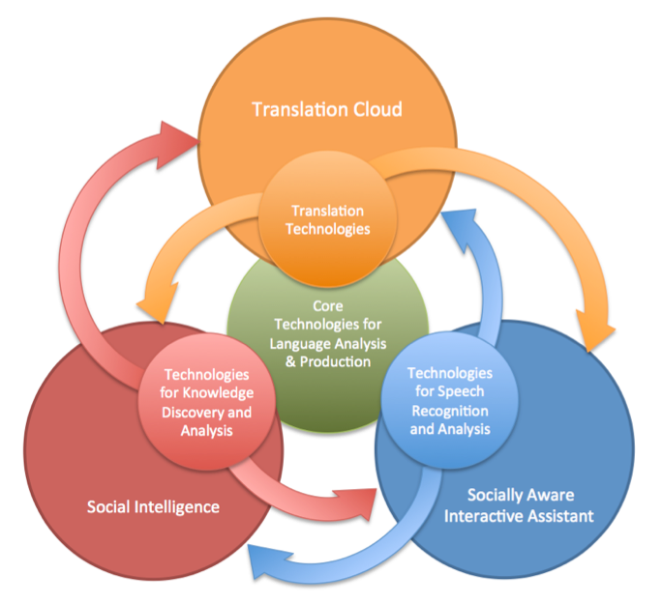
\includegraphics[width=0.75\textwidth]{../_media/PT-Rings}
  \caption{Scientific cooperation among the three priority research themes}
  \label{fig:priority-themes}
  \colorrule{grey3}{\textwidth}{1.5pt}
\end{figure*}

Except for a few large national projects and programmes such as Techno-langue and Quaero in France, Verbmobil and Theseus in Germany and DARPA Communicator and GALE in the US the field of language technology does not have experience with research efforts of the scope required for the targeted advances and plans in this SRA.  Nevertheless, our technology area has to follow developments in other key engineering disciplines and speed up technology evolution by massive collaboration based on competitive division of labour and sharing of resources and results. In our reflection on optimal schemes for organizing we tried to draw lessons from our own field’s recent history and to capitalize on experience from other fields by adopting approaches that proved successful and evading encountered pitfalls.
 
The final model for the organisation of collaboration will have to be guided by a thoughtful combination of the following basic approaches.
 
\textbf{Flexible collaborative approach:}  For each priority theme, one or several very large cooperating and competing or coopetiting lead projects will share an infrastructure for evaluation, resources (data and base technologies), and communication. Mechanisms for reducing or terminating partner involvements and for adding new partners or subcontracted contributors should provide the needed flexibility. A number of smaller projects including some national and regional projects will provide needed building blocks for particular languages, tasks, component technologies or resources. A special cooperation scheme will be designed for effectively involving EC-funding, contributions from member states, industrial associations, and language communities. The choice of the funding instruments will be determined in due time after.

\textbf{Staged approach:} Two or three major phases are foreseen. For better concertation the major phases should be synchronized among the projects.   

\textbf{Evolutionary approach:} Instead of banking on one selected paradigm, a number of competing approaches will be followed in parallel with shared efficient schemes for evaluation, merging, adopting and discontinuing research threads so that the two elements of successful evolutionary research approaches, selection and cross-fertilization, are exploited to the maximum possible.

\textbf{Analytical approach:} Instead of the currently predominant search for an ideal one-fits-all approach, the research will focus on observed quality barriers and not shun computationally expensive dedicated solutions for overcoming particular obstacles.

\textbf{Bootstrapping approach:} Better systems can be derived from more and better data and through new insights. Improved systems can also be used to gain better data and new insights. Thus the combination of the analytical evolutionary approach with powerful machine learning techniques will be the basis for a technology bootstrapping, which has been the by far most fruitful scheme for the development of highly complex technologies.

\textbf{Close cooperation of language technology and relevant areas of service and technology industries:} In order to increase chances of successful commercialisation and to obtain convincing and sufficiently tested demonstrations of novel applications, the relevant industrial sectors of industry must be strongly integrated into the entire research cycle.

\textbf{Tighter research-innovation cycle:} Through the collaboration between research, commercial services and commercial technology industries, especially through the shared evaluation metrics and continuous testing, the usual push-model of technology transfer will hopefully substituted by a pull-model, in which the commercial technology users can ask for specific solutions. In the envisaged research scheme incentives will be created for competing teams each composed of researchers, commercial users and commercial developers by the participating enterprises for initiating successful innovations

\textbf{Interdisciplinary approach:} A number of science, technology and service areas need to be integrated into the research from day one. Some technology areas such as speech technologies, language checking and authoring systems need to be represented by providers of state-of-the-art commercial products.

Supporting research and innovation in language technology should be accompanied by policy making in the area of multilingualism, but also in digital accessibility. Overcoming language barriers can greatly influence the future of the EU. Solutions for better communication and for access to content in the native languages of the users would reaffirm the role of the EC to serve the needs of the EU citizens. A substantial connection to the infrastructural program CEF could help to speed up the transfer of research results to badly needed services for the European economy and public.
 
At the same time, use cases should cover areas where the European societal needs massively overlap with business opportunities to achieve funding investment that pays back, ideally public-private partnerships.
 
The coordination among the three priority research strands poses additional administrative challenges. Because of the described interdependencies and also because of the need to maintain and improve the obtained level of cohesion and community spirit in the European LT community, a coordinating body is needed. Whether such an entity is jointly carried by the three areas or by a separate support project, needs to be determined in the upcoming discussion on the appropriate support instruments for the identified research priorities.

% FIXME: The following text (until the beginning of the next subsection) was the final piece in Stelios' input on the LR/infrastructural aspects which follows imediately after.

% FIXME: This piece of text _must_ be modified, currently it's much too strong and much too prominent. META-SHARE is there but this short text argues to create another META-SHARE?! Has to be made more vague!

% FIXME: This section and the following one clash with the "European Service Platform". Way too many platforms!

In order to optimise the efficiency of the shared core technologies for language analysis and production as well as the basic infrastructural development, maximise the infrastructure's impact, and ensure that requirements for research and development are met at the necessary depth for all languages in all priority themes, the organisation of the infrastructural initiative (see Section~\ref{sec:sharing-resources-and-results}) should adopt the following principles:

\begin{itemize}
\item It is necessary to invest substantial efforts in the development of integrated infrastructure platforms based on open architectures, enabling the sharing and development, as needed, of the necessary resources.
\item Such platforms should enable developed resources, data and related processing services to be incorporated in, or called by a wide range of application software.
\item Such platforms should support technology specific challenges/shared tasks in order to accelerate innovation breakthrough and market-readiness for desperately needed technologies.
\item Concerted activities and policies facilitating the sharing of resources catering for all stumbling blocks on the way to technical, organisational and legal interoperability should be supported.
\item EU level research should be aligned with efforts on the national level, so that language coverage is efficiently achieved.
\item To boost the automation of the language resource acquisition process, thus increasing coverage, quality and adequacy, a small number of coordinating projects attached to a ‘federation of STREPs’ with complementary goals can be foreseen. These projects should be objective-driven, with clear research, technology and exploitation milestones, coordinated by an ongoing road-mapping effort.
\item In order to increase research efficiency within a public-private partnership, the preferred infrastructure should handle the various applications in connection with the cooperative development of technologies, including regular objective evaluation of technology progress, and the production of the appropriate resources which are necessary to develop and test the various technologies.
\end{itemize}

\subsection{Shared Research Results, Infrastructures, Resources and Technologies}
\label{sec:sharing-resources-and-results}

% FIXME: the following paragraph is old text

By now the European academic and industrial technology community is fully aware of the need for sharing resources such as language data (e.\,g., text and speech corpora), language descriptions (e.\,g., lexicons, thesauri, grammars), tools (e.\,g., taggers, stemmers, tokenizers) and core technology components (e.\,g., morphological, syntactic, semantic processing). Initiatives like ELRA, FLaReNet, and CLARIN have prepared the ground for this culture of sharing, META-NET's open resource exchange infrastructure, called META-SHARE, is providing the technological platform as well as legal and organisational schemes.

% The remainder of this section is based on Stelios' input (sent on June 29, 2012)

The successful implementation of the three aforementioned priority themes and the delivery of the respective applications and services to the EU citizen depend on the appropriate infrastructure through which the necessary language resources, language data and basic language processing tools are made available for training models, developing and evaluating systems and services. As is evident from the priority descriptions, some of the required datasets and tools are independent of the individual priorities and the underlying technologies, as they provide development support through basic modules for language modeling at various levels (raw corpora, morphosyntactically annotated corpora, transcribed speech corpora, etc). Other types of resources, such as error-annotated corpora for machine translation, spoken dialogue corpora, etc, are priority specific.  The European academic and industrial technology community is aware of the need for and benefits from sharing resources such as language data (e.g. text and speech corpora), lexical resources (e.g. computational lexica, terminology databases, ontologies, thesauri), language descriptions (e.g. language models, grammars), tools (e.g. taggers, stemmers, tokenizers) and core technology components (e.g. morphological, syntactic, semantic processing) as a basis for the successful development and implementation of the research priorities.

From the point of view of resource availability and distribution, sharing can be seen as a synonym of Data Openness, i.e. data that are easily obtainable and can be used with few, if any, restrictions. However, reluctance in fully embracing an open resources model is still common. Deeper understanding of the pros and cons of closing or opening up language resources is needed, as well as a capillary educational action at all levels.

The resources issue varies considerably for languages other than English. Some are relatively well covered when there are programmes that provide the investments needed to produce data, basic language processing tools and evaluation systems.

Realizing the appropriate multilingual LR infrastructure needs a collaborative and coordinated effort from all stakeholders. While there has been considerable progress in technology developments in the last decade, the significant challenge of overcoming current fragmentation and imbalance inside the LTs community for all languages still remains an issue. This effort should revolve around the following axes: Infrastructure; Coverage, Quality, Adequacy; Language Resources Acquisition; Openness; Interoperability.

\subsubsection{Infrastructure}
\label{sec:infrastructure}

Building and maintaining a sustainable facility for sharing resource data and tools, such as META-SHARE is a priority. Broad participation is essential in maintaining and extending the infrastructure, so that acceptance by the public and contributors is ensured. This infrastructure will help, in primis, to make language resources available, visible and easily accessible. Second, the infrastructure will facilitate sharing and exchange of language resources. 

The basic principles of an infrastructure for language resources and technologies require a community approach that brings together and builds on current experiences and endeavours. It is necessary to define and agree on the basic criteria and dimensions for an appropriate governance, and define the basic data and software resources that should populate this infrastructure. Multilingual coverage, the capacity to attract providers of useful and usable resources, improvements in sharing mechanisms, and collaborative working practices between R\&D and commercial users are key aspects. There must also be a business-friendly framework to stimulate the commercial use of these resources, based on a sound licensing facility, ease of access, ease of conversion into uniform formats. 

The content of the infrastructure should not be limited to data, though. Instead, it has to be seen as an international hub of resources and technologies for speech and language services from industries and communities. The development and proposal of (free) tools and more generally Web services (comparable to the Language Grid), including evaluation protocols and collaborative workbenches is deemed essential in such LR infrastructure. The accumulation and sharing of resources and tools in a single place would lower the cost of R\&D for new applications in new language resource domains.

Sustainability covers preservation, accessibility, and operability (among other things) that all have mutual influences. Collecting and preserving knowledge in the form of existing LRs should be a key priority.
LRs must be accessible over the long term. A sustainability analysis must be part of a resource specification phase, and it is important that funding agencies impose a sustainability plan mandatory for those projects that are concerned with production of language resources.

Accurate and reliable documentation of Language Resources is an undisputable need. An effort must be made to collect all existing LR documentation and make it easily available. To this end, the maintenance of a (virtual) repository of specifications, guidelines, and documentation of LRs, starting with reference resource models or widely known and used resources. Documentation is also the gateway to LR discovery. Ensuring that Language Resources are discoverable is the first step towards promoting the data economy. In order to make LRs discoverable, language resource providers (LRPs) should always document their resources, using standard metadata and unique resource identifiers. 

\subsubsection{Coverage, Quality, Adequacy}
\label{sec:cover-qual-adeq}

With the current data-driven paradigm in force, innovation in LT nowadays crucially depends on language resources. Despite the vast amount of academic and industrial investment, there are not enough available resources to satisfy the needs of all languages, quantitatively and qualitatively. Language resources should be produced and made available for every language, every register, every domain to guarantee full coverage, high quality and adequacy for the various LT applications. New methods of resource development can be exploited to achieve better coverage, for instance shared or distributed ones. It is important to assess the availability of existing resources with respect to their adequacy to applications and technology requirements. This involves assessing the maturity of the technologies for which new resources should be developed.
Specifically for the advancement of LTs, Basic Language Resource Kits (or BLARKs) should be supported and developed for all languages and, at least, main applications (Machine Translation, Information Retrieval, Question Answering to mention a few). Also, as many of the undocumented languages of our cultural legacy may become extinct in the digital age, minority and fringe languages should be comprehensively represented through spoken and written corpora, and manuscripts should be digitized.

To this end and to reduce the amount of human intervention and revision, automatic techniques should be promoted to guarantee quality through error detection and confidence assessment. The promotion of validation and evaluation can perform a valuable role in fostering the improvement of formal and content quality of resources. Evaluation should encompass technologies, resources, guidelines and documentation. But like the technologies it addresses, evaluation is constantly evolving, and new, more specific measures using innovative methodologies are needed to evaluate the reliability of language resources, while maximal use of existing tools should be ensured for the automatic or semi-automatic formal and content validation of LRs. Requirements for language resource quality are to be assessed by a think-tank composed by recognized experts from a broad spectrum of the community.

The entire ecosystem around Language Resources needs substantial support and recognition. A “Language Resources Impact Factor (LRIF)” should be defined in order to enforce the practice of citation of resources on the model of scientific paper authoring and to calculate actual research impact of resources.
A reference model for creating Language Resources instead will help address the current shortage of resources in terms of breadth (languages and applications) and depth (data quality and volume). Such reference model should also include an accurate estimate of the production costs.

\subsubsection{Language Resources Acquisition}
\label{sec:lang-reso-acqu}

Re-use and re-purposing via a “recycling” culture should be encouraged to ensure the reuse of development methods, existing tools, and translation/transliteration tools, etc. With production costs constantly increasing, there is a need to invest in innovative production methods that massively involve automatic procedures, so as to reduce human intervention to a minimum. The coverage problem is so enormous that strategies that approach or ensure full automation for (high-quality) LR data production should be promoted. It is worth considering the power of social/collaborative media to build resources, especially for those languages where there are no language resources built by experts yet.  

There are several promising experiments in crowd-sourcing data collection and NLP tasks. Crowd-sourcing makes it possible to mobilize large armies of human talent around the world with just the right language skills so that it is feasible to collect what we need when we need it. For instance, it has been estimated that Mechanical Turk translation is 10 to 60 times less expensive than professional translation. 

A particularly sensitive case is that of less-resourced languages, where language technology should be developed rapidly to help minority-language speakers access education and the Information Society. Basic language resources for all the world’s languages could be created building a Web 2.0 site (using the same community computing power that generates millions of blogs) starting with the 446 languages currently present on the web. Collaborative and Web 2.0 methods for data collection and annotation seem particularly very well-suited for collecting the data needed for the development of LT applications. 

\subsubsection{Openness}
\label{sec:openness}

There is strong impulse towards open data nowadays, in the sense of data that are easily obtainable and can be used with few, if any, restrictions. To share resources, both data and tools, has become a viable solution towards encouraging open data, and the community is strongly investing in facilities for the discovery and use of resources by federated members. These facilities, such as the META-SHARE infrastructure, could represent an optimal intermediate solution to respond to the needs for data variety, ease of retrieval, better data description and community-wide access, while at the same time assisting in clearing the intricate issues associated with intellectual property rights.

The challenge for both the language technology community and policy makers is to push for the development of a common legal framework that would facilitate resource sharing efforts abiding by the law, benefiting from the adoption of “fair use” principles and appropriate copyright exceptions.  It is of foremost importance that legislation regarding LR use be harmonised, and even standardised, for all types of LRs, and that free use of LRs be allowed, at least for research or non-profit purposes. Licensing schemes need to be simplified through broad-based solutions for both R\&D and industry. Electronic licensing (e-licenses) should be adopted and current distribution models to new media (web, mobile devices, etc.) should be accepted.

\subsubsection{Interoperability}
\label{sec:interoperability}

Interoperability of resources seeks to maximise the extent to which they are compatible and therefore integratable at various levels, so as to allow, for instance, the merging of data or tools coming from different sources, while preserving their semantics and individual functions. Interoperability of resources and data is also an essential prerequisite for successful exploitation of the enormous amount of data that the advent of the Internet has been making available since less than two decades. The community and funding agencies need to join forces to drive forward the use of existing and emerging standards, at least in the areas where there is some degree of consensus. The only way to ensure useful feedback to improve and advance is to use these standards on a regular basis. It will be thus even more important to enforce and promote the use of standards at all stages, from basic standardisation for less-resourced languages (such as orthography normalization, transcription of oral data, etc.) to more complex areas (such as semantics, etc.). Language Resource producers, on their side, should look for standards and best practices that best fit the LRs to be produced, already at the early stages of design/specifications.

% ------- End of Stelios' text

\subsection{Mechanisms for Showcasing and Innovation}
\label{sec:powerf-mech-showcasing-and-innovation}

Language Technology is innovation-friendly in the sense that many solutions are not standardised, but require individual adaptation or new development for a certain customer or application. Thus, one can truly speak of socially responsible innovation here.

As there are many niches in the market that are not targeted by the big players, SMEs do have real opportunities. At the same time, as a key-enabling technology, language technology usually enters the markets in combination with other technologies as an essential component of novel products and services that can be arbitrarily complex and big, which has made it difficult for SMEs to identify customers in the past.    

The question is how to transform innovation and research into new markets, products, growth, and, finally, new jobs. In recent years, drivers for innovations have often been applications and tools such as Skype, Facebook, or recommender systems that have been designed by smaller teams and start-ups. Important aspects of their success stories, besides the core and novel functionalities and feature sets for which there was an obvious need, was often their fast and viral outreach and uptake through social networks. The trend towards widely used platforms has drastically facilitated spreading innovative technologies.

Large global platforms for novel end-user-services have also become the predominant innovation drivers for language technology solutions. These platforms can be web-services such as Google search that integrates the new Knowledge Graph concept network, speech-enabled search and web-translation. They could also be hardware/OS combinations such as iOS 6 for Apple’s mobile devices with its speech-activated assistant Siri. Or it could be an open operating system such as Android that is expected to extend its current speech and language functionalities in the near future.

The trend towards widely used platforms will drastically facilitate spreading innovative language technologies. Actually, language technology has a good chance of becoming the essential feature for the success of the next generation of services. At closer inspection, the integration of sophisticated language technology in current platforms is rather limited, scratching only the surface of what will be possible in the near future.

\subsection{A European Service Platform for Language Understanding, Communication, Knowledge, Inference and Emotion}
\label{sec:europ-service-platform}

In this section we argue for the creation of an ambitious large-scale sky-computing platform as a central motor for research and innovation in the next phase of IT evolution and a ubiquitous resource for the multilingual European society (an idea suggested by several experts from industry in META-NET Vision Group meetings). The platform will be used for testing, show casing, proof-of-concept demonstration, avant-garde adoption, experimental and operational service composition, and fast and economical service delivery to enterprises and end-users.
 
The proposed creation of a powerful cloud or sky computing platform for a wide range of services dealing with human language, knowledge and emotion will not only benefit the individual and corporate users of these technologies but also the providers.
 
Users will be able to receive customized integrated services without having to install, combine, support and maintain the software. They will have access to specialized solutions even of they do not use these regularly. 
 
\textbf{Language technology providers} will have ample opportunity to offer services stand-alone or integrated with others.
 
\textbf{Providers of language services} rendered by human language professionals will be able to use the platform for enhancing their services by means of appropriate technology and for providing their services stand-alone or integrated into other application services.
 
\textbf{Researchers} will have a unique virtual laboratory for testing, combining, and benchmarking their novel technologies and for exposing them in realistic trials to real tasks and end users.
 
\textbf{Providers of services} that can be enabled or enhanced by text and speech processing will utilize the platform for testing the needed LT functionalities
and for integrating them into their own solutions.
 
In order to allow for the gigantic range of foreseeable and currently not yet foreseeable solutions, the infrastructure will have to host all relevant simple services, including components, tools and data resources, as well as various layers or components of higher services that incorporate simpler ones.
 
A top layer consists of \textbf{language} processing such as text filters, spell checking, hyphenation, lemmatizing and parsing. At a slightly deeper level, services will be offered that realize some degree and form of language \textbf{understanding} including entity and event extraction, opinion mining and translation. Both basic language processing and understanding will be used by services that support human \textbf{communication} or realize some human-machine interaction. Part of this layer are question answering and dialogue systems as well as email response applications. Another component will bring in services for processing and storing \textbf{knowledge} gained by and used for understanding and communication. This part will include repositories of linked data and ontologies, as well as services for building, using and maintaining them. These in turn permit a certain range of rational capabilities often attributed to a notion of intelligence. The goal is not to model the entire human intelligence but rather to realize selected forms of \textbf{inference} that are needed for utilizing and extending knowledge, for understanding and for successful communication. These forms of inference permit better decision support, pro-active planning and autonomous adaptation. A final part of services will be dedicated to human \textbf{emotion}.  Since people are largely guided by their emotions and strongly affected by the emotions of others, truly user-centred IT need facilities for detecting and interpreting emotion and even for expressing emotional states in communication.
 
Because of its components (language, understanding, communi­cation, know­ledge, inference and emotion) we subsume the entire set of services under the acronym LUCKIE.  We consider the paradigm of federated cloud services or sky computing with its emerging standards such as OCCI, OVM and CDMI and toolkits such a OpenNebula as the appropriate approach for realizing the ambitious infrastructure.  
 
All three priority areas of the SRA will be able to contribute to and at the same time draw immense benefits from this platform. There are strong reasons for aiming at a single service platform for the three areas and for the different types of technologies. They share many basic components and they need to be combined for many valuable applications, including the selected showcase solution of the three areas.

\subsubsection{Implementation of the Platform}
\label{sec:implementation-of-platform}

The creation of the Platform has to be supported by public funding. Because of the high requirements concerning performance, reliability, user support, scalability, persistence as well as data protection and conformance with privacy regulation, the platform needs to be established by a consortium with strong commercial partners and also be operated by this consortium or a commercial contractor. A similar platform with slightly different desiderata and functionalities is currently built under the name Helix-Nebula for the Earth Sciences with the help of the following commercial partners: Atos, Capgemini, CloudSigma, Interoute, Logica, Orange Business Services, SAP, SixSq, Telefonica, Terradue, Thales, The Server Labs and T-Systems. Partners are also the Cloud Security Alliance, the OpenNebula Project and the European Grid Infrastructure. These are working together with major research centres in the earth sciences to establish the targeted federated and secure high-performance computing cloud platform.
 
The intended platform for LT and neighbouring fields would be intended for a mix of commercial and non-commercial services. It would be cost-free for all providers of non-commercial services (cost-free and advertisement-free) including research systems, experimental services and freely shared resources but it would raise revenues by charging a proportional commission on all commercially provided services.  In order to reduce dependence on individual companies and software products, the base technology should be supplied by open toolkits and standards such as OpenNebula and OCCI.  
 
For each of the three priority research themes, chances for successful showcasing and successful commercial innovation will increase tremendously if usable services could be offered on such a platform of required strength and reliability.
 
The platform will considerably lower the barrier for market entry for innovative technologies, especially for products by SMEs. Still, these stakeholders May not have the resources, expertise, and time to create the necessary interfaces to integrate their results into real-life services, let alone the overarching platform itself. There is still a gap between research prototypes and products that have been engineered and tested for robust applications. Moreover, many innovative developments require access to special kind of language resources such as recordings of spoken commands to smartphones, which are difficult to get for several reasons.
 
Thus the service platform will be an important instrument for supporting the entire innovation chain, but in addition interoperability standards, interfacing tools, middle ware, reference service architectures need to be developed and constantly adapted. Many of these may not be generic enough to serve all application areas, so that much of the work in resource service integration will have to take place in the respective priority theme research actions.

% FIXME: Integrate the following paragraphs?

% The LUCKIE SKY will put the barrier for market entry of language technology research projects and SMEs much lower than it used to be in the past. Still, these stakeholders do not have the resources, expertise, and time to create the necessary interfaces to integrate their results into real-life services, let alone the overarching platform itself. There is still a gap between research prototypes and products that have been engineered and tested for robust applications. Moreover, many innovative developments require access to special kind of language resources such as recordings of spoken commands to smartphones, which are difficult to get for several reasons. 

% The LUCKIE SKY has to be supported by public funding. Project funding could include space in its app store and possibly also testing capacities using methods such as Amazon’s mechanical turk. The best applications could at a later stage be tested by public services or test users. For each of the three priority research themes, chances for successful showcasing and successful commercial innovation will increase tremendously if usable services could be offered on such a platform of required strength and reliability. With the help and support of the European language technology industry, such a platform can actually be built and put to use. It will serve as a major enabling factor for successful commercialization in Europe. 

% Apart from new ways of sharing, development, and distribution, a generally innovative climate is needed. The availability of venture capital and meeting points like summits where research and decision makers from industry get together should be backed by public funding, and uptake. Flexible funded consortia that run over a longer period with changing partners, where research and innovation phases lead over to product development and marketing would also support innovation.

\end{multicols}

% --------------------------------------------------------------------------

\clearpage

\appendix
\addtocontents{toc}{\protect\smallskip}

% ===========================================================================

\ssection[References]{References}
\bibliographystyle{unsrt}
\bibliography{sra_references}

\clearpage

% ===========================================================================

\ssection[List of Key Contributors]{List of Key Contributors}
\label{sec:list-of-contributors}

In the following we list the experts who contributed to this Strategic Research Agenda (55\% from Language Technology User or Provider Industries, 49\% from Language Technology Research, 2,3\% from national or international institutions).

% Academia: 64
% Industry: 72
% Other:     3 (EPO, JRC, Ministry of Defense, France)

\begin{multicols}{3}
\begin{small}
  \begin{enumerate}
    \raggedright{
      \item Sophia Ananiadou, University of Manchester, UK
      \item Toni Badia, Barcelona Media, Spain
      \item Michaela Bartelt, Electronic Arts, Germany/USA
      \item Christoph Bauer, ORF, Austria
      \item Nozha Boujemaa, INRIA, France
      \item Hervé Bourland, IDIAP, Switzerland
      \item Antonio Branco, University of Lisbon, Portugal
      \item Andrew Bredenkamp, acrolinx, Germany
      \item Gerhard Budin, University of Vienna, Austria
      \item Axel Buendia, Spir.\,Ops, France
      \item Aljoscha Burchardt, DFKI, Germany
      \item Will Burgett, Intel, USA
      \item Johannes Bursch, Daimler AG, Germany
      \item Nicoletta Calzolari, Consiglio Nazionale delle Ricerche, Italy
      \item Nick Campbell, Trinity College Dublin, Ireland
      \item Jean Carrive, INA, France
      \item Khalid Choukri, ELDA, France
      \item Philipp Ciminiano, University of Stuttgart, Germany
      \item Ann Copestake, University of Cambridge, UK
      \item Ido Dagan, Bar-Ilan University, Israel
      \item Morena Danieli, Loquendo, Italy
      \item Claude de Loupy, Syllabs, France
      \item Maarten de Rijke, University of Amsterdam, The Netherlands
      \item Marin Dimitrov, Ontotext, Bulgaria
      \item Petar Djekic, SoundCloud, UK
      \item Bill Dolan, Microsoft, USA
      \item Christoph Dosch, Institut für Rundfunktechnik, Germany
      \item Marcello Federico, FBK, Italy
      \item David Filip, Moravia, Czech Republic
      \item Dan Flickinger, Stanford University, USA
      \item Gil Francopoulo, CNRS/LIMSI and IMMI, France
      \item Piotr W. Fuglewicz, Micro, Poland
      \item Robert Gaizauskas, University of Sheffield, UK
      \item Martine Garnier-Rizet, CNRS/LIMSI and IMMI, France
      \item Simon Garrett, British Telecom, UK
      \item Stefan Geissler, Temis, Germany
      \item Edouard Geoffrois, Ministry of Defense and French National Research Agency, France
      \item Yota Georgakopolou, European Captioning Institute, UK
      \item Serge Gladkoff, Logrus International and GALA Standards Director, USA/Russia
      \item Daniel Grasmick, Lucy Software, Germany
      \item Gregory Grefenstette, Exalead, France
      \item Marko Grobelnik, Institut ``Jožef Stefan'', Slovenia
      \item Joakim Gustafson, KTH Royal Institute of Technology, Sweden
      \item Jan Hajic, Charles University Prague, Czech Republic
      \item Paul Heisterkamp, Daimler AG, Germany
      \item Mattias Heldner, KTH Royal Institute of Technology, Sweden
      \item Manuel Herranz, PangeaMT, Spain
      \item Theo Hoffenberg, Softissimo, France
      \item Thomas Hofmann, Google, Switzerland/USA
      \item Timo Honkela, Aalto University, Finland
      \item Krzysztof Jassem, Poleng, Poland
      \item Keith Jeffery, Science and Technology Facilities Council, Rutherford Appleton Lab., UK
      \item Kristiina Jokinen, University of Helsinki, Finland
      \item Rebecca Jonson, Artificial Solutions, Spain
      \item John Judge, Dublin City University and CNGL, Ireland
      \item Martin Kay, Stanford University, USA and Universität des Saarlandes, Germany
      \item Christopher Kermorvant, A2iA, France
      \item Simon King, University of Edinburgh, UK
      \item Philipp Koehn, University of Edinburgh, UK
      \item Maria Koutsombogera, ILSP, Greece
      \item Steven Krauwer, University of Utrecht, The Netherlands
      \item Verena Krawarik, APA, Austria
      \item Stefan Kreckwitz, Across, Germany
      \item Simon Krek, Institut ``Jožef Stefan'', Slovenia
      \item Brigitte Krenn, OFAI, Austria
      \item Michal Küfhaber, Skrivanek, Czech Republic
      \item Jimmy Kunzmann, EML, Germany
      \item Bernardo Magnini, FBK, Italy
      \item Gudrun Magnusdottir, ESTeam, Sweden
      \item Elisabeth Maier, CLS Communication, Switzerland
      \item Joseph Mariani, CNRS/LIMSI and IMMI, France
      \item Penny Marinou, Litterae Trans, Greece
      \item Margaretha Mazura, EMF, UK/Belgium
      \item Wolfgang Menzel, University of Hamburg, Germany
      \item Roger Moore, University of Sheffield, UK
      \item Sukumar Munshi, Across, Germany
      \item Bart Noe, Jabbla, The Netherlands
      \item Jan Odijk, University of Utrecht, The Netherlands
      \item Stephan Oepen, University of Oslo, Norway
      \item Karel Oliva, Czech Academy of Sciences, Czech Republic
      \item Mehmed Özkan, Bogazici University, Turkey
      \item Maja Pantic, Imperial College London, UK
      \item Alexandre Passant, DERI, Ireland
      \item Pavel Pecina, Dublin City University and CNGL, Ireland
      \item Manfred Pinkal, Universität des Saarlandes, Germany
      \item Stelios Piperidis, ILSP, Greece
      \item László Podhorányi, Vodafone, Hungary
      \item Jörg Porsiel, VW, Germany
      \item Gabor Proszeky, Morphologic, Hungary
      \item Artur Raczynski, European Patent Office, Germany
      \item Georg Rehm, DFKI, Germany
      \item Steve Renals, University of Edinburgh, UK
      \item Peter Revsbech, Ordbogen, Denmark
      \item Giuseppe Riccardi, University of Trento, Italy
      \item Johann Roturier, Symantec, Ireland
      \item Dimitris Sabatakakis, Systran, France
      \item David Sadek, Institute Telecom, France
      \item Sergi Sagàs, MediaPro, Spain
      \item Felix Sasaki, W3C and DFKI, Germany
      \item Jana Šatková, ACP Traductera, Czech Republic
      \item Mirko Silvestrini, Rapidrad, Italy
      \item Ruud Smeulders, Rabo Bank, The Netherlands
      \item Svetlana Sokolova, ProMT, Russia
      \item Juan Manuel Soto, Fonetic, Spain
      \item Lucia Specia, University of Sheffield, UK
      \item C.\,M.~Sperberg-McQueen, W3C and BlackMesa Technologies, USA
      \item Volker Steinbiss, RWTH Aachen and Accipio, Germany
      \item Rudi Studer, KIT, Germany
      \item Katerina Stuparicova, Charles University Prague, Czech Republic
      \item Daniel Tapias, Sigma Tech, Spain
      \item Alessandro Tescari, Pervoice, Italy
      \item Lori Thicke, Translators without Borders and Lexcelera, France
      \item Gregor Thurmair, Linguatec, Germany
      \item Rudy Tirry, Lionbridge, Belgium
      \item Hans Uszkoreit, DFKI and Universität des Saarlandes, Germany
      \item Erik van der Goot, Joint Research Center, EC, Italy
      \item Peggy van der Kreeft, Deutsche Welle, Germany
      \item Jaap van der Meer, TAUS, The Netherlands
      \item René van Erk, Wolters Kluwer, The Netherlands
      \item Josef van Genabith, Dublin City University and CNGL, Ireland
      \item Arjan van Hessen, Twente University and Telecats, The Netherlands
      \item David van Leeuwen, TNO and Radboud University, The Netherlands
      \item Andrejs Vasiljevs, Tilde, Latvia
      \item Michel Vérel, VecSys, France
      \item Claire Waast, EDF, France
      \item Philippe Wacker, EMF, UK/Belgium
      \item Wolfgang Wahlster, DFKI, Germany
      \item Alex Waibel, KIT, Germany and CMU, Jibbigo, USA
      \item Jakub Zavrel, Textkernel, The Netherlands
      \item Elie Znaty, VecSys, France
      \item Chenqing Zong, Chinese Academy of Sciences, China
    }
  \end{enumerate}
\end{small}
\end{multicols}
  
\clearpage

% --------------------------------------------------------------------------

\ssection[About META-NET]{About META-NET}

% FIXME: Include the "three stripes" visual in this chapter

\begin{multicols}{2}
\textbf{META-NET} is a Network of Excellence funded by the European Commission \cite{rehm2011}.  The network currently consists of 60 members in 34 European countries. META-NET forges \textbf{META}, the Multilingual Europe Technology Alliance, a growing community of language technology professionals and organisations in Europe. META-NET fosters the technological foundations for a truly multilingual European information society that:

\begin{itemize}
\item makes communication and cooperation possible across languages;
\item grants all Europeans equal access to information and knowledge regardless of their language; 
\item builds upon and advances functionalities of networked information technology.
\end{itemize}

The network supports a Europe that unites as a single digital market and information space. It stimulates and promotes multilingual technologies for all European languages. These technologies support automatic translation, content production, information processing and knowledge management for a wide variety of subject domains and applications. They also enable intuitive language-based interfaces to technology ranging from household electronics, machinery and vehicles to computers and robots.

Launched on 1 February 2010, META-NET has already conducted various activities in its three lines of action META-VISION, META-SHARE and META-RESEARCH. 

\textbf{META-VISION} fosters a dynamic and influential stakeholder community that unites around a shared vision and a common strategic research agenda (SRA). The main focus of this activity is to build a coherent and cohesive LT community in Europe by bringing together representatives from highly fragmented and diverse groups of stakeholders. The present white paper was prepared together with volumes for 29 other languages. The shared technology vision was developed in three sectorial Vision Groups. The META Technology Council was established in order to discuss and to prepare the SRA based on the vision in close interaction with the entire LT community.

\textbf{META-SHARE} creates an open, distributed facility for exchanging and sharing resources. The peer-to-peer network of repositories will contain language data, tools and web services that are documented with high-quality metadata and organised in standardised categories. The resources can be readily accessed and uniformly searched. The available resources include free, open source materials as well as restricted, commercially available, fee-based items. 

\textbf{META-RESEARCH} builds bridges to related technology fields. This activity seeks to leverage advances in other fields and to capitalise on innovative research that can benefit language technology. In particular, the action line focusses on conducting leading-edge research in machine translation, collecting data, preparing data sets and organising language resources for evaluation purposes; compiling inventories of tools and methods; and organising workshops and training events for members of the community.

\vfill
%\centerline{office@meta-net.eu -- http://www.meta-net.eu}
\textbf{\centerline{office@meta-net.eu -- http://www.meta-net.eu}}
\end{multicols}

\clearpage

% ===========================================================================

\ssection[Members of META-NET]{Members of META-NET}
\label{metanetmembers}

\small

\begin{longtable}{@{}lp{137mm}@{}}
Austria & Zentrum für Translationswissenschaft, Universität Wien: Gerhard Budin\\ \addlinespace 
Belgium & Centre for Processing Speech and Images, University of Leuven: Dirk van Compernolle \\ \addlinespace
& Computational Linguistics and Psycholinguistics Research Centre, University of Antwerp: \newline Walter Daelemans\\ \addlinespace
Bulgaria & Institute for Bulgarian Language, Bulgarian Academy of Sciences: Svetla Koeva \\ \addlinespace
Croatia & Institute of Linguistics, Faculty of Humanities and Social Science, University of Zagreb: Marko Tadić \\ \addlinespace
Cyprus & Language Centre, School of Humanities: Jack Burston \\ \addlinespace
Czech Republic & Institute of Formal and Applied Linguistics, Charles University in Prague: Jan Hajič \\ \addlinespace
Denmark & Centre for Language Technology, University of Copenhagen: Bolette Sandford Pedersen, \newline Bente Maegaard\\ \addlinespace
Estonia & Institute of Computer Science, University of Tartu: Tiit Roosmaa, Kadri Vider\\ \addlinespace
Finland & Computational Cognitive Systems Research Group, Aalto University: Timo Honkela\\ \addlinespace
& Department of Modern Languages, University of Helsinki: Kimmo Koskenniemi, Krister Lindén \\ \addlinespace
France & Centre National de la Recherche Scientifique, Laboratoire d'Informatique pour la Mécanique et les Sciences de l'Ingénieur and Institute for Multilingual and Multimedia Information: Joseph Mariani \\ \addlinespace
& Evaluations and Language Resources Distribution Agency: Khalid Choukri\\ \addlinespace
& Laboratory of Computer Science, University of Le Mans: Holger Schwenk\\ \addlinespace
& Laboratoire Informatique d'Avignon, University of Avignon: Georges Linares\\ \addlinespace
Germany & Language Technology Lab, DFKI: Hans Uszkoreit, Georg Rehm\\ \addlinespace 
& Human Language Technology and Pattern Recognition, RWTH Aachen University: Hermann Ney \\ \addlinespace 
& Department of Computational Linguistics, Saarland University: Manfred Pinkal\\ \addlinespace
& Institute for Natural Language Processing, University of Stuttgart: Jonas Kuhn, Hinrich Schütze\\ \addlinespace
& Interactive Systems Lab, Karlsruhe Institute of Technology: Alex Waibel\\ \addlinespace 
Greece & R.C. “Athena”, Institute for Language and Speech Processing: Stelios Piperidis\\ \addlinespace
Hungary & Research Institute for Linguistics, Hungarian Academy of Sciences: Tamás Váradi\\  \addlinespace
& Department of Telecommunications and Media Informatics, Budapest University of Technology and Economics: Géza Németh, Gábor Olaszy\\ \addlinespace
Iceland & School of Humanities, University of Iceland: Eiríkur Rögnvaldsson\\ \addlinespace
Ireland & School of Computing, Dublin City University: Josef van Genabith\\ \addlinespace
Italy & Consiglio Nazionale delle Ricerche, Istituto di Linguistica Computazionale “Antonio Zampolli”: \newline Nicoletta Calzolari\\ \addlinespace
& Human Language Technology Research Unit, Fondazione Bruno Kessler:  Bernardo Magnini\\ \addlinespace 
Latvia & Tilde: Andrejs Vasiļjevs\\ \addlinespace  
& Institute of Mathematics and Computer Science, University of Latvia: Inguna Skadiņa\\ \addlinespace
Lithuania & Institute of the Lithuanian Language: Jolanta Zabarskaitė\\ \addlinespace
Luxembourg & Arax Ltd.: Vartkes Goetcherian\\ \addlinespace
Malta & Department Intelligent Computer Systems, University of Malta: Mike Rosner\\ \addlinespace
Netherlands & Utrecht Institute of Linguistics, Utrecht University: Jan Odijk\\ \addlinespace  
& Computational Linguistics, University of Groningen: Gertjan van Noord\\ \addlinespace
Norway & Department of Linguistic, Literary and Aesthetic Studies, University of Bergen: Koenraad De Smedt\\ \addlinespace  
& Department of Informatics, Language Technology Group, University of Oslo:  Stephan Oepen \\ \addlinespace
Poland & Institute of Computer Science, Polish Academy of Sciences: Adam Przepiórkowski, Maciej Ogrodniczuk \\ \addlinespace
& University of Łódź: Barbara Lewandowska-Tomaszczyk, Piotr Pęzik\\ \addlinespace
& Dept.~of Comp.~Linguistics and Artificial Intelligence, Adam Mickiewicz University: Zygmunt Vetulani \\ \addlinespace
Portugal & University of Lisbon: António Branco, Amália Mendes \\ \addlinespace 
& Spoken Language Systems Laboratory, Institute for Systems Engineering and Computers: Isabel Trancoso \\ \addlinespace
Romania & Faculty of Computer Science, University Alexandru Ioan Cuza of Iași: Dan Cristea \\ \addlinespace
& Research Institute for Artificial Intelligence, Romanian Academy of Sciences:  Dan Tufiș \\ \addlinespace
Serbia  & University of Belgrade, Faculty of Mathematics: Duško Vitas, Cvetana Krstev,  Ivan Obradović \\ \addlinespace
& Pupin Institute: Sanja Vranes \\ \addlinespace  
Slovakia & Ľudovít Štúr Institute of Linguistics, Slovak Academy of Sciences: Radovan Garabík \\ \addlinespace 
Slovenia & Jožef Stefan Institute: Marko Grobelnik \\ \addlinespace 
Spain & Barcelona Media: Toni Badia, Maite Melero \\ \addlinespace  
& Aholab Signal Processing Laboratory, University of the Basque Country:  Inma Hernaez Rioja \\ \addlinespace 
& Center for Language and Speech Technologies and Applications, Universitat Politècnica de Catalunya:  Asunción Moreno \\ \addlinespace 
& Department of Signal Processing and Communications, University of Vigo:  Carmen García Mateo \\ \addlinespace 
& Institut Universitari de Lingüística Aplicada, Universitat Pompeu Fabra: Núria Bel \\ \addlinespace 
Sweden & Department of Swedish, University of Gothenburg: Lars Borin \\ \addlinespace 
Switzerland & Idiap Research Institute: Hervé Bourlard \\ \addlinespace 
UK & School of Computer Science, University of Manchester: Sophia Ananiadou \\ \addlinespace  & Institute for Language, Cognition and Computation, Center for Speech Technology Research, University of Edinburgh: Steve Renals \\ \addlinespace 
& Research Institute of Informatics and Language Processing, University of Wolverhampton:\newline Ruslan Mitkov \\ \addlinespace
& Department of Computer Science, University of Sheffield: Rob Gaizauskas\\ 
\end{longtable}
\normalsize

\renewcommand*{\figureformat}{}
\renewcommand*{\captionformat}{}

\begin{figure*}[h]
  \colorrule{grey3}{\textwidth}{1.5pt}
  \center
  %\fbox{-- META-NET group picture omitted to keep the size of the PDF file small. --}
  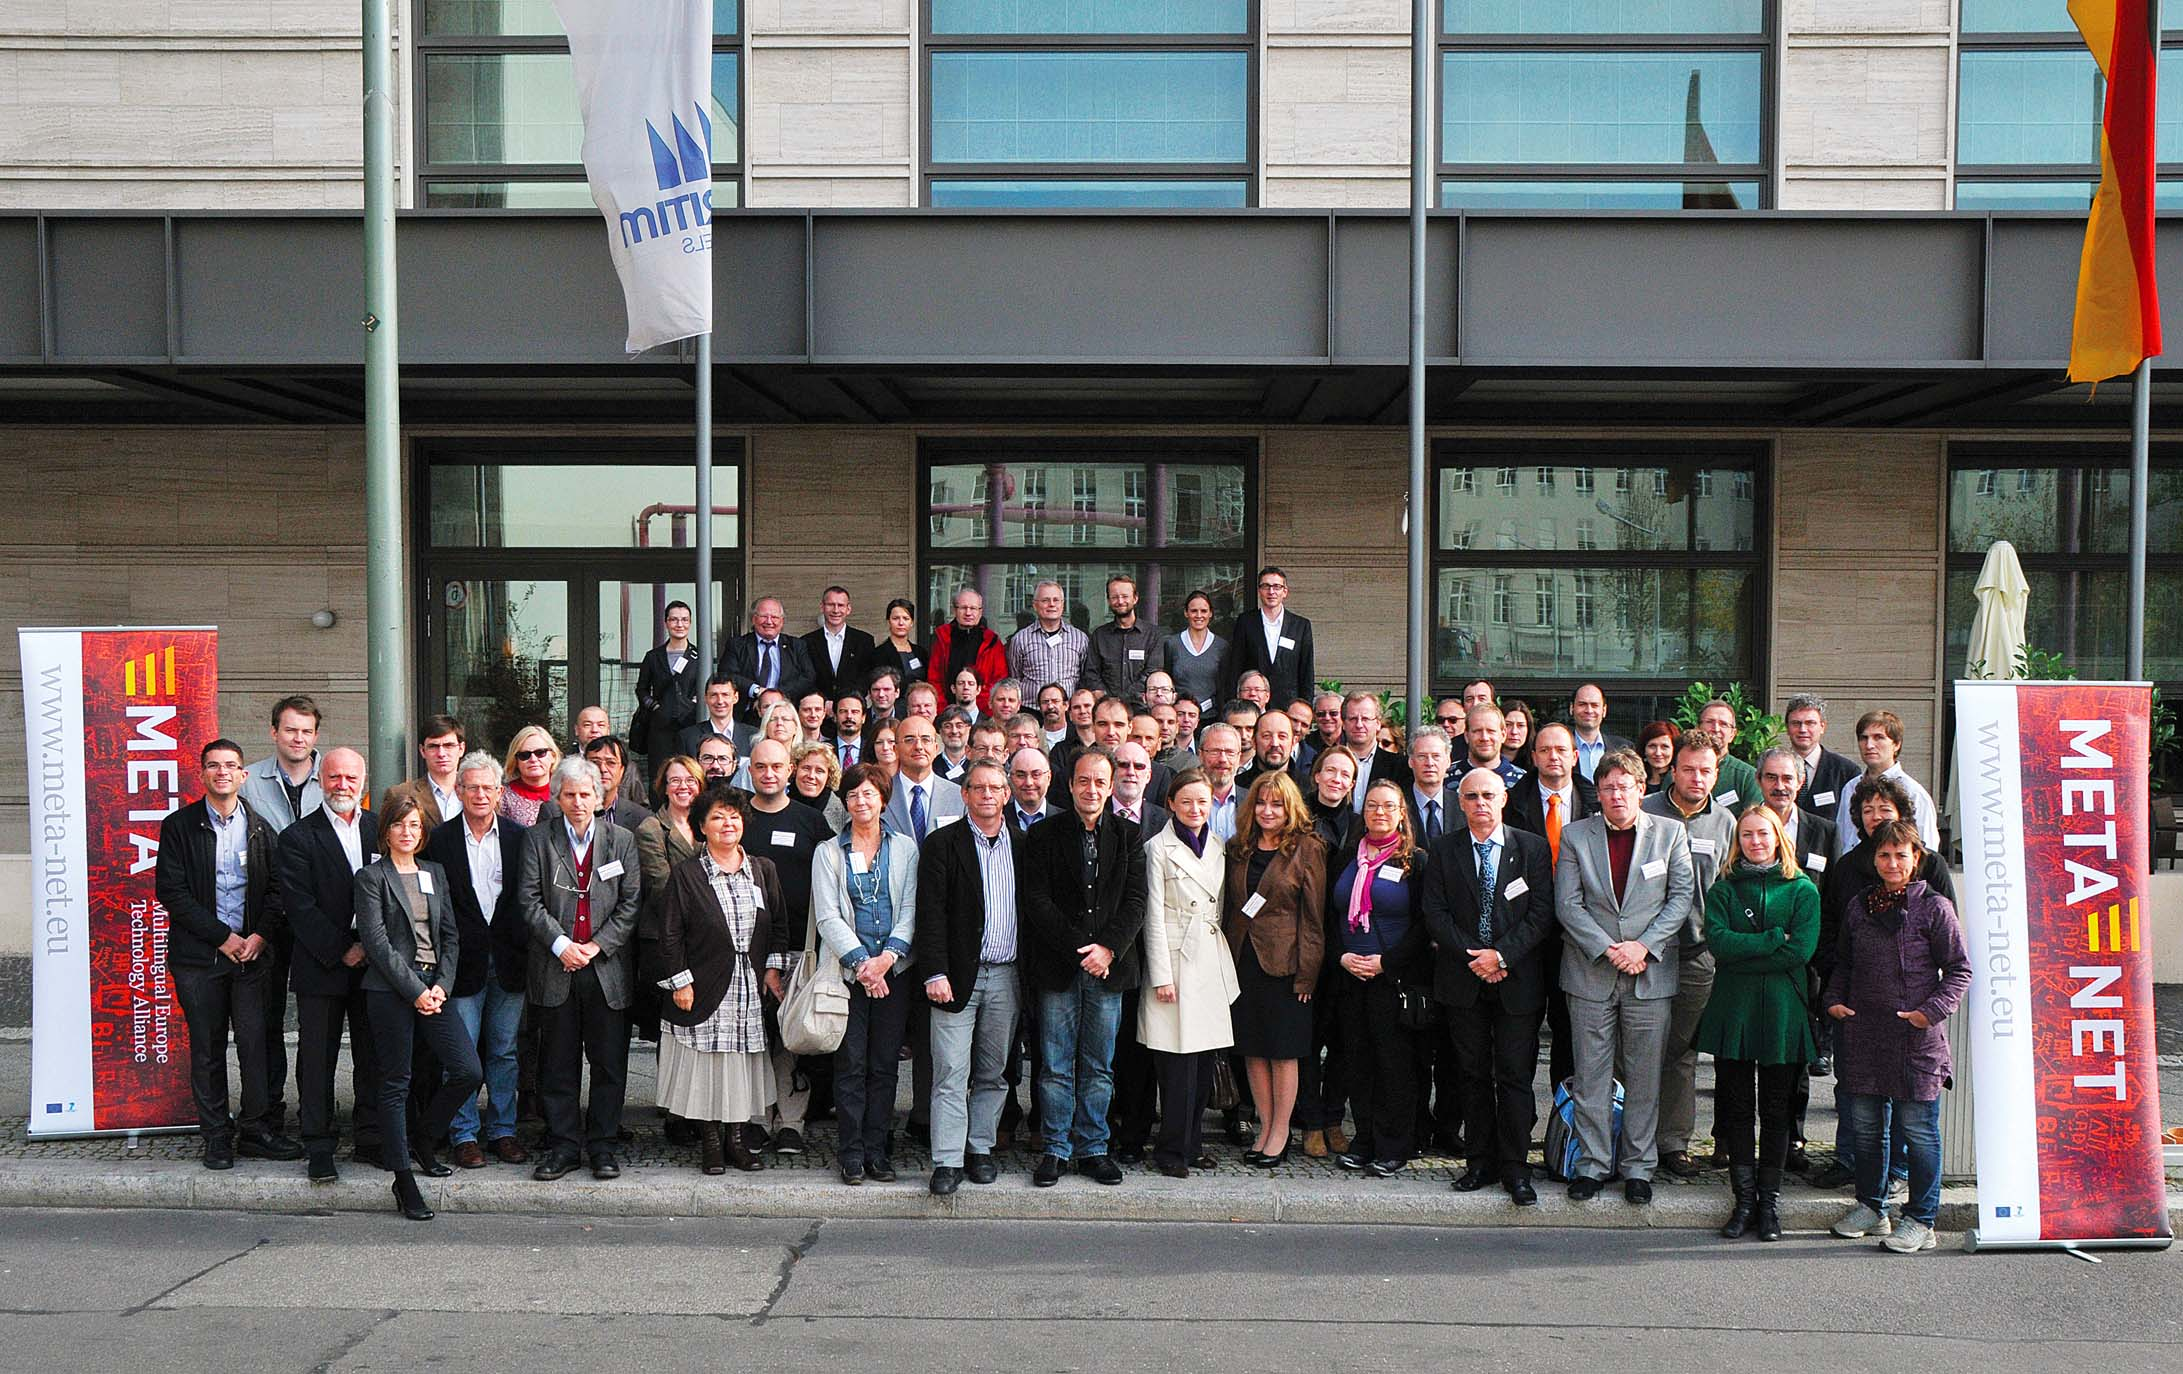
\includegraphics[width=\textwidth]{../_media/meta-net_team.jpg}
  \caption{About 100 language technology experts -- representatives of the countries and languages represented in META-NET -- discussed and finalised the key results and messages of the White Paper Series at a META-NET meeting in Berlin, Germany, on October 21/22, 2011.}
  \medskip
  \colorrule{grey3}{\textwidth}{1.5pt}
\end{figure*}

\clearpage

% ===========================================================================

%\ssection[Members of META]{Members of META}
%\label{metamembers}

% FIXME: Include a very tightly typeset list of the 630+ META members

%\clearpage

% ===========================================================================

\ssection[Milestones and History of the Strategic Research Agenda]{Milestones and History of the\newline Strategic Research Agenda}
\label{vision-evolution}

The META-VISION process within META-NET started in early 2010, its main aim was to produce this Strategic Research Agenda and the accompanying Roadmap document. Hundreds of representatives from academia, industry, official institutions, policy makers, politicians and journalists have contributed to this process. In this section we give an overview of the meetings at which the SRA or important components on the way towards the SRA have been presented and discussed (key meetings of the META-VISION process marked in bold typeface). 

Important milestones within the long and complex process towards this Strategic Research Agenda include five documents: the three Vision Reports prepared by the three domain-specific Vision Groups (see below), a general Vision Paper, ``The Future European Multilingual Information Society: Current State of the Discussion'' \cite{Meta1}, and the Priority Themes Paper in which the three technology visions are specified in a more concrete way, ``LT 2020 -- Vision and Priority Themes for Language Technology Research in Europe until the Year 2020. Towards the META-NET Strategic Research Agenda'' \cite{LT2020}. All reports, papers and discussions that took place in the process have been reflected in the Strategic Research Agenda. The documents are available online at \url{http://www.meta-net.eu/vision}.

\begin{small}
\begin{enumerate}
\item FLaReNet Forum, Barcelona, Spain, Feb.~11/12, 2010
\item Language Technology Days 2010, Luxembourg, March 22/23, 2010
\item EAMT 2010, Saint-Raphael, France, May 27/28, 2010
\item theMETAnk, Berlin, Germany, June 4/5, 2010
\item Translingual Europe 2010, Berlin, Germany, June 7, 2010
\item Localization World, Berlin, Germany, June 8/9, 2010
\item Multisaund Seminar, Istanbul, Turkey, June 16-18, 2010
\item \textbf{Vision Group ``Text Translation and Localisation''} (1st meeting), Berlin, Germany, July 23, 2010
\item \textbf{Vision Group ``Media and Information Services''} (1st meeting), Paris, France, Sep.~10, 2010
\item \textbf{Vision Group ``Interactive Systems''} (1st meeting), Paris, France, Sep.~10, 2010
\item ICT 2010, Brussels, Belgium, September 27-29, 2010
\item \textbf{Vision Group ``Text Translation and Localisation''} (2nd meeting), Brussels, Belgium, Sep.~29, 2010
\item \textbf{Vision Group ``Interactive Systems''} (2nd meeting), Prague, Czech Republic, Oct.~5, 2010
\item Languages and the Media 2010, Berlin, Germany, October 7, 2010
\item HLT: The Baltic Perspective, Riga, Latvia, October 7/8, 2010
\item LISA Forum Europe, Budapest, Hungary, October 13, 2010
\item \textbf{Vision Group ``Media and Information Services''} (2nd meeting), Barcelona, Spain, Oct.~15, 2010
\item EFNIL 2010, Thessaloniki, Greece, Nov.~3, 2010
\item Interact Presidential Summit, Moffett Field, USA, Nov.~8-9, 2010
\item \textbf{META Technology Council} (1st meeting), Brussels, Belgium, Nov.~16, 2010
\item Language question in research: English vs.~national languages?, Finnish Parliament, Helsinki, Nov.~17, 2010
\item \textbf{META-FORUM 2010: ``Challenges for Multilingual Europe''}, Brussels, Belgium, Nov.~17/18, 2010
\item Oriental-Cocosda 2010, Kathmandu, Nepal, Nov.~24-25, 2010
\item The International Workshop on Spoken Language Translation (IWSLT), Paris, France, Dec.~2/3, 2010
\item Meeting of the LT Berlin working group, Berlin, Germany, Dec.~9, 2010
\item Language Technology for Multilingual Applications, European Parliament, Luxembourg, Jan.~27, 2011
\item Opening of German/Austrian W3C Office at DFKI Berlin, Berlin, Germany, Feb.~10, 2011
\item Japanese Workshop for Machine Translation, Tokyo, Japan, Feb.~23, 2011
\item Meeting of Representatives of European Language Councils, Copenhagen, Denmark, March 08, 2011
\item TRALOGY, Paris, France, March 3/4, 2011
\item \textbf{Vision Group ``Interactive Systems''} (3rd meeting), Rotterdam, The Netherlands, March 28, 2011
\item \textbf{Vision Group ``Media and Information Services''} (3rd meeting), Vienna, Austria, April 1, 2011
\item Meeting of the LT Berlin working group, Berlin, Germany, April 4, 2011
\item W3C Workshop ``Content on the multilingual web'', Pisa, Italy, April 5, 2011
\item \textbf{Vision Group ``Translation and Localisation''} (3rd meeting), Prague, Czech Republic, April 7/8, 2011
\item Attensity Forum 2011, Berlin, Germany, May 6, 2011
\item \textbf{META Technology Council} (2nd meeting), Venice, Italy, May 25, 2011
\item FLaReNet Forum, Venice, May 26-27, 2011
\item Multisaund Seminar, Bursa, Turkey, June 13-14, 2011
\item META-NET Workshop at ICANN 2011: Context in Machine Translation,
Espoo, Finland, June 14, 2011
\item Speech Processing Conference, Tel Aviv, Israel, June 21-22, 2011
\item \textbf{META-FORUM 2011: ``Solutions for Multilingual Europe''}, Budapest, Hungary, June 27/28, 2011
\item Media for All, London, June 29-July 1, 2011
\item EUROLAN 2011 Summer School, Cluj-Napoca, Romania, Aug.~28-Sep.~4, 2011
\item Interspeech 2011, Firenze, Italy, Aug.~28-31, 2011
\item RANLP 2011, Hissar, Bulgaria, Sep.~12-14, 2011
\item Multilingual Web Workshop, Limerick, Ireland, Sep.~21/22, 2011
\item ML4HMT Workshop at MT Summit, Xiamen, China, Sep.~19-23, 2011
\item Workshop Language Technology for a Multilingual Europe at GSCL 2011, Hamburg, Germany, Sep.~27, 2011
\item GSCL 2011: ``Multilingual Resources and Multilingual Applications'', Hamburg, Germany, Sep.~28-30, 2011
\item \textbf{META Technology Council} (3rd meeting), Berlin, Germany, Sep.~30, 2011
\item Workshop on IPR and Metadata by META-NORD, Helsinki, Finland, Sep.~30, 2011
\item META-NET Network Meeting and General Assembly, Berlin, Germany, Oct.~21/22, 2011
\item NPLD Assembly, Eskilstuna, Sweden, Oct.~25/26, 2011
\item EFNIL 2011, London, UK, Oct.~26, 2011
\item Oriental-Cocosda 2011, Hsinchu, Taiwan, Oct.~26-28, 2011
\item SIMC 2011 International Symposium on Multilingualism in the Cyberspace, Brasilia, Brasil, Nov.~7-9, 2011
\item IJCNLP 2011, Chiang Mai, Thailand, Nov.~9-13, 2011
\item ML4HMT-11 Workshop, Barcelona, Spain, Nov.~19, 2011
\item LTC 2011, Poznan, Poland, Nov.~25-27, 2011
\item GALA Conference, Monaco, March 26-29, 2012
\item EACL 2012, Avignon, France, April 23-27, 2012
\item CESAR Roadshow Event, Sofia, Bulgaria, May 2, 2012
\item LREC 2012, Istanbul, Turkey, May 21-27, 2012
\item CESAR Roadshow Event, Bratislava, Slovakia, June 7/8, 2012
\item Multilingual Web Workshop, Dublin, Ireland, June 11, 2012
\item \textbf{META Technology Council} (4th meeting), Brussels, Belgium, June 19, 2012
\item \textbf{META-FORUM 2012: ``A Strategy for Multilingual Europe''}, Brussels, Belgium, June 20/21, 2012
\item CHAT 2012 Workshop, Madrid, Spain, June 22, 2012
\end{enumerate}
\end{small}

\begin{figure*}[htb]
  \colorrule{grey3}{\textwidth}{1.5pt}
  \center
  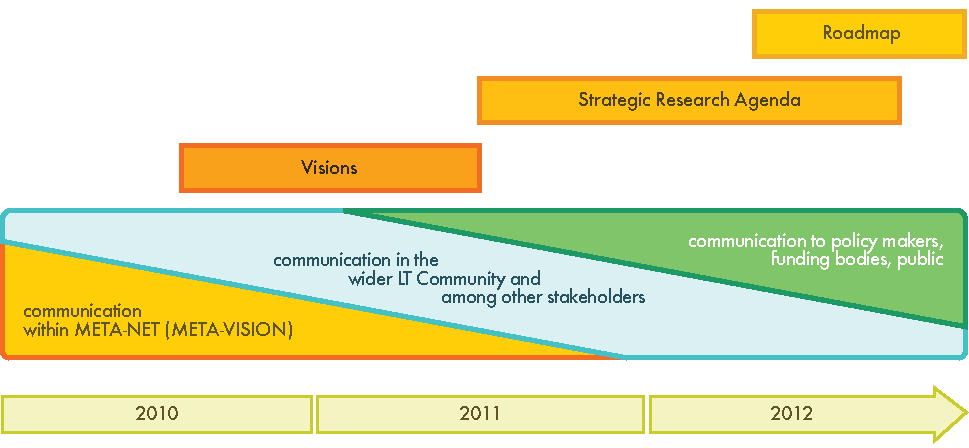
\includegraphics[width=0.65\textwidth]{../_media/Timeline}
  \caption{The three phases of the META-VISION process}
  \label{fig:sra-timeline}
  \colorrule{grey3}{\textwidth}{1.5pt}
\end{figure*}
 
\begin{figure*}[htb]
  \colorrule{grey3}{\textwidth}{1.5pt}
  \center
  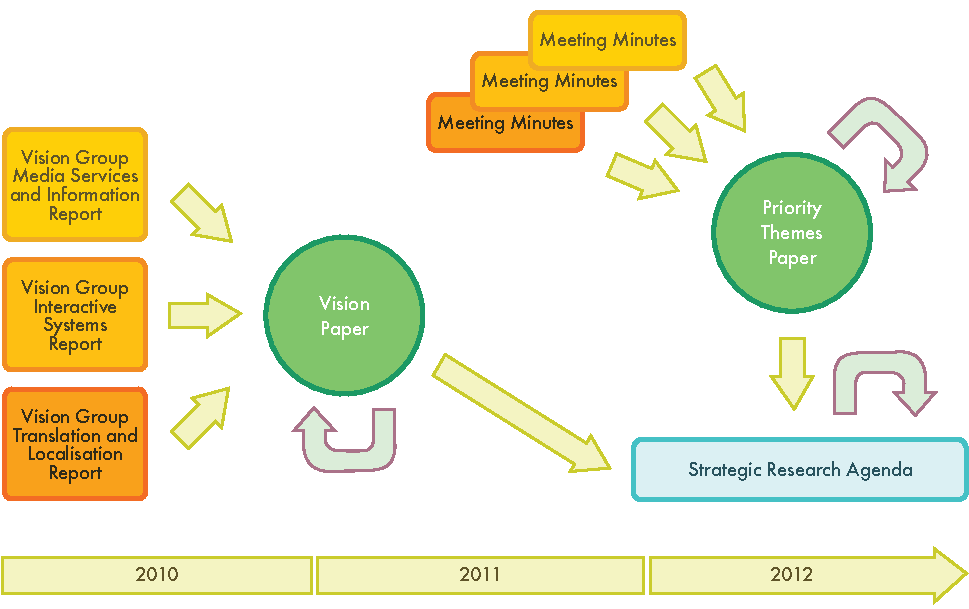
\includegraphics[width=0.65\textwidth]{../_media/Towards-SRA}
  \caption{Steps towards the Strategic Research Agenda for Multilingual Europe 2020}
  \label{fig:towards-sra}
  \colorrule{grey3}{\textwidth}{1.5pt}
\end{figure*}

\clearpage

% ===========================================================================

\ssection[LT for Europe's Languages: The Funding Situation]{LT for Europe's Languages:\newline The Funding Situation}
\label{european-funding-situation}

% FIXME: The following contains a collection of raw findings per language from the Language White Papers. The collection needs to be completed and the content still needs to be aggregated and integrated into the main text.

% FIXME: If we decide to keep this appendix we should write a short introduction to explain where this info is coming from.

\begin{multicols}{2}

\begin{small}
\subsection*{Basque}
\label{sec:basque}

Since 2000 up till today, the Spanish Government supported within the National Plan of Research and Technology several projects in the area of Multilingual Speech Technologies: TEHAM, AVIVAVOZ, and BUCEADOR. Their main purpose was to improve the quality of Speech Recognition, Speech Translation and Text to Speech Synthesis in all the official languages spoken in Spain: Basque, Galician, Catalan and Spanish.

\subsection*{Bulgarian}
\label{sec:bulgarian}

The first international and national funding supporting language technologies for Bulgarian began at the very beginning of 1990s. Over a short period of time financing for a number of research projects from European institutions was got: LaTeSLav (Language Processing Technologies for Slavic Languages, 1991-1994) aimed at developing a prototype of a grammar checker, BILEDITA (Bilingual Electronic Dictionaries and Intelligent Text Alignment, 1996-1998) for the development of bilingual electronic dictionaries, GLOSSER (Support of Second Language Acquisition and Learning from Aligned Corpora, 1996-1998) aimed at supporting foreign language training and others. The Multext-East (Multilingual Text Tools and Corpora for Central and Eastern European Languages, 1995-1997) extension of the previous Multext and EAGLES (European Commission’s Expert Advisory Group on Language Engineering Standards) EU projects provided the Bulgarian language resources in a standardised format with standard mark-up and annotation, and these resources were later expanded and upgraded in the ELAN (European Language Activity Network, 1998-1999), TELRI I in II (Trans European Language Resources Infrastructure, 1995-1998 / 1999-2001) and Concede (Consortium for Central European Dictionary Encoding, 1998-2000) projects. Bulgarian institutions are also involved in the CLARIN project (Common Language Resources and Technology Infrastructure). Other ongoing projects include those comprised by EUROPEANA aimed at developing the basic technologies and standards necessary to make knowledge on the Internet more widely available in the future.

\subsection*{Catalan}
\label{sec:catalan}

Machine translation, speech recognition, spelling and grammar checking research and industrial developments have been supported by different departments of the Generalitat de Catalunya for more than 20 years. The CREL – Centre de Referència en Enginyeria Lingüística, 1996-2000, managed by the Institut d’Estudis Catalans and with participants from the major Catalan Universities, was created with the specific aim of promoting the creation of resources and tools for the automatic processing of Catalan texts in a variety of applications. As regards the presence of the Catalan language in European infrastructures, in 2008 the Catalan Government signed an agreement with Universitat Pompeu Fabra, the national representative of the European project CLARIN in Spain, with the aim of building a Catalan demonstrator. In addition, the Biblioteca de Catalunya, Catalonia’s national library, is one of the partners in the EUROPEANA project. From 2000 up until the present day, the Spanish Government supported several projects in the area of multilingual speech technologies within the National Plan of Research and Technology, i.e., TEHAM, AVIVAVOZ, and BUCEADOR. The main purpose of these projects was to improve the quality of speech recognition, speech translation and text to speech synthesis in all the official languages spoken in Spain, i.e., Basque, Galician, Catalan and Spanish. In 2005, the Catalan Government launched a project to produce Language Resources for Speech Recognition and Speech Synthesis. As a result, Language Resources for telephone applications, in-car applications and microphone applications were produced. Later, the project TECNOPARLA (2007-2010) had as its objective the translation of speech between Spanish and Catalan. The project resulted on advances in all the component speech technologies, i.e. diarization, speech recognition, speech translation and text to speech synthesis.

%\subsection*{Croatian}
%\label{sec:croatian}
%
%n.\,a.

\subsection*{Czech}
\label{sec:czech}

Most of the government-originating funding programs are maintained by the Czech Science Foundation (GAÈR) and focused on basic research. Recently (2009), a new Technological Agency of the Czech Republic (Technologická agentura Èeské republiky, TAÈR) has been established, which shall focus on applied research. However, there are probably no LT-related projects funded by TAÈR yet. 

\subsection*{Danish}
\label{sec:danish}

The Research Council for the Technical Sciences had speech technology as one of the main themes in their strategy plan for 1998-2002, and they did support several language technology projects. The inter-disciplinary IT research programmes running from mid 1990s to 2003 have been able to support a few language technology related projects (as was the case for OntoQuery and SIABO), but have not had a specific aim to do so.
The Research Agency of the Danish Ministry for Science, Technology and Development decided in 2001 to promote language technology by funding a collaborative effort to enlarge the Danish language technology lexicon developed in the European PAROLE project. The resulting dictionary (STO) is now available through ELRA, and is being used for research and commercial purposes. It was the specific aim of the Research Agency to support the Danish language in the digital age, by granting funds for the development of basic language technology building blocks.
In parallel with the ESFRI initiative for research infrastructure, Denmark has started a roadmap process for research infrastructures. One of the research infrastructures to be supported will be a “Digital Humanities Laboratory” for the support of humanities research through the use of language technology.

\subsection*{Dutch (Netherlands, Flanders)}
\label{sec:dutch-neth-fland}

Activities for the Dutch language have been promoted and supported in several programmes and projects over the last one and a half decade. Thus a Dutch language spoken train information system was developed as a carrier for research in speech analysis and generation, in language analysis and generation, and in dialogue management in the OVIS programme in the late nineties. 

METAL produced a Dutch-French MT system for the ministries of Agriculture and Internal Affairs, and after the Dutch Language Union issued a call for the development of MT systems translating between Dutch on the one hand and English and French on the other in 1999, funded by public money, Systran developed such systems in the context of the NL-Translex project. In the IOP MMI (Innovation Research Programme on Man Machine Interaction) and CATCH programs language and speech technology have been used as tools for man machine interfaces and disclosing cultural heritage.

Most prominent in their focus on the Dutch language are the joint Netherlands-Flanders CGN and STEVIN programmes. These have yielded significant progress in the availability of basic resources (data and tools) for the Dutch language, some initial research and several end user applications. Though some of the results achieved in these projects can be exploited in industry and in academia (e.g. in the CLARIN-NL research infrastructure) the prospects for optimally exploiting these results in actual research and in industry further are grim. 

\subsection*{English}
\label{sec:english}

AKT (2000-2007), was a multi-million pound collaboration between five UK universities, with the aim of enhancing information and knowledge management in the age of the World Wide Web. The research conducted on the project formed an important contribution to the semantic web, in which the use of LT technologies played a central role. A follow-up project, ”EnAKTing the Unbounded Data Web: Challenges in Web Science”, is currently ongoing.
Two systems which support the user in creating new applications from existing libraries of processing components are the University of Sheffield’s GATE system, which has been under development for over 15 years, and the more recent UCompare system, which was developed as part of a collaboration between the Universities of Tokyo, Manchester and Colorado. Whilst current components in UCompare mainly deal with English, the library will be extended as part of META-NET to cover a number of different European languages.

%\subsection*{Estonian}
%\label{sec:estonian}
%
%n.\,a.

\subsection*{Finnish}
\label{sec:finnish}

Public support from TEKES has been an important source of funding for basic research especially through two large technology programs, USIX (User-Oriented Information Technology) 1999--2002 and FENIX (Interactive Computing) 2003--2007. Some of the core technologies identified in the program in UNIX were Finnish speech recognition, large data management and search interfaces.

NLP projects carried out within the FENIX technology program include FENIX 4M (Mobile and Multilingual Maintenance Man) and FinnONTO (Semantic Web Ontologies) at the University of Helsinki, New methods and applications in speech processing and Search-in-a-Box (University of Turku), Rich semantic media for personal and professional users (VTT Technical Research Centre of Finland) and Intelligent Web Services (Helsinki School of Science and Technology), StatHouse Semantics and Automatic content classification and ontologies (Seerco Ltd).  Recently, A joint project on speech synthesis between the University of Helsinki and Aalto University has been very successful in the new field of statistical parametric synthesis based on Hidden Markov Models and a new, physiologically grounded vocoding technology.

EU funded projects in Finland since the 1980’s include LR SIMPLE, LR PAROLE and EU MLIS 5008 LINGMACHINE. The Common Language Resources and Technologies Infrastructure (CLARIN) was funded by the Commission during 2008 - 2010, and the work within the initiative continues. The national part FINCLARIN is funded by the Ministry of Education and Culture.  HFST (Helsinki Finite State Transducer Technology), OMor (Open Source Morphologies), FinnWordNet, and FinnTreeBank are examples of currently ongoing projects.

\subsection*{French (France, Belgium, Switzerland, Canada)}
\label{sec:french-france-belg}

As a follow-up of the FRANCIL program of the AUPELF-UREF (Francophone Universities Association) from 1994 to 2000, the Techno-Langue program (2003-2005), supported by the Ministries of Research, Industry and Culture, included the development of Language Resources (corpus, lexica, dictionaries, etc.) for French and the organization of 8 evaluation campaigns, on topics such as Syntactic Parsing, Text Alignment, Machine Translation, Terminology Extraction, Information Retrieval (Question \& Answer), Broadcast News speech transcription (ESTER campaign), Text-to-Speech Synthesis and Spoken dialog. The ESTER campaign allowed producing, in 2004, 1,700 hours of Broadcast News speech in French, 100 hours of which have been transcribed, making it possible to develop Broadcast News transcription systems of sufficient quality and opening the feasibility of automatic video transcription and indexing for French.  Some of those activities are now continuing as individual projects supported by the ANR (ETAPE, PASSAGE, PORT MEDIA), which also organized the REPERE challenge on multimodal (text, speech and vision) person identification (2010-2013).

CNRS (the National Centre for Scientific Research) had several programs in that field along the years, and the French Ministry for Research settled in 2011 a Corpus Infrastructure in the Human and Social Sciences area, in connection with the EC CLARIN project.

Nowadays, OSEO supports the very large Quaero program gathering 31 industrial and academic partners (French and German) with a total budget of 200 M. and an amount of public funding of 99 M. over 5 years (2008-2013). Quaero addresses the development of around 30 technologies for various medias (speech, text, music, image, video) for the needs of 8 applications related to Multimedia and Multilingual Document processing (Digitization platform, Multimedia Entreprise Capture, Social impact media monitoring, Personalized video, Communication portals \& Digital Heritage, Online Translation Platform, Real Life Mobile Search and Multimedia search engines). All technologies are developed under a strict, regular quantitative evaluation scheme, while a special project produces the data that is necessary for developing and testing the technologies. Although the program mostly addresses the French language, some technologies will be developed for most of the 23 EU official languages. The Voxalead News online application developed by Dassault/Exalead in cooperation with LIMSI-CNRS, Vocapia Research and INRIA is a good example of a major technological achievement made possible within Quaero by gathering know-how in three different areas (search engines, speech processing and image processing). 

In Belgium, the Service de la langue de la Communaute francaise de Belgique has funded the development of terminological researches in the past and is officially in charge of coordinating the terminological activities (at the government level) in the Francophone part of Belgium. The OWIL (Observatoire du Traitement Informatique des Langues et de l’Inforoute) has centralized information on NLP research and activities for several years, but has stopped its activities in 2008.

There is currently no major LTR program in Switzerland.  The most relevant project may be the National Centre of Competence in Research on Interactive Multimodal Information Management (IM2), lead by IDIAP, where speech corpora have been collected, mainly in collaboration with the EC AMI and AMIDA projects. There used to be an “observatoire” for research, but the site is now inactive. 

Canada has a special agency for HLT: the LTRC (Language Technology Research Center) / CRTL (Centre de Recherche en Technologies Langagières). There are in Canada several academic teams working on HLT, but without any specific national program, apart from generic national research programs.

\subsection*{Galician}
\label{sec:galician}

The Centre for the Development of Industrial Technology (CDTI) is a Spanish public organisation, under the Ministry of Science and Innovation, whose objective is to help Spanish companies increase their technological profile. CDTI evaluates and finances R\&D projects through programmes such as CENIT and AVANZA.

The CENIT (National Strategic Consortiums for Technological Research) programme seeks to stimulate public and private-sector cooperation in R\&D. Information Technology and Communication is one of the programme’s priority areas. Projects in this area sometimes include research in Language Technologies.

The aim of the AVANZA Plan is to bring the Information Society to ordinary citizens, and to private and public sectors. Among their priorities is to facilitate the use of new technologies to elderly people and people with disabilities. User-friendly language technology tools offer the principal solution to satisfy this goal, for example by offering speech synthesis for the blind.

The Galician Regional Government supports research through the “Plan Galego de Investigación, Desenvolvemento e Innovación Tecnolóxica (PGIDIT)”. Language Technology is not a priority line, but along the years research groups from the universities and some companies have gotten grants for doing research and developments in LT.

\subsection*{German (Germany, Austria, Switzerland)}
\label{sec:germ-germ-austr}

COLLATE, funded by the BMBF from 2000 to 2006, was one of the first projects to address the issues of a language infrastructure and led to the creation of an information portal for the field (LT World). German and Austrian institutions are involved in the on-going European CLARIN project. Other on-going projects include EUROPEANA and THESEUS, a project co-funded by the Federal Ministry of Economics and Technology (BMWI) that aims to develop the basic technologies and standards needed to make knowledge on the Internet more widely available in the future.

In Austria, the Faculty of Computer Sciences at the University of Vienna is carrying out the JETCAT project on translation between Japanese and English, and an on-going project has been compiling the Austrian Academy Corpus since 2001. There are no dedicated LT programmes in Austria. Funding for LT-related topics typically comes from research programmes that have open topics, especially those that focus on the transfer of knowledge from academic research to industry (particularly via SMEs). Several of these programmes are administered by the Austrian Research Promotion Agency (FFG). The Vienna Science and Technology Fund (WWTF) is a fairly strong supporter of localised LT, especially for topics related to Vienna, such as synthesizing the speech of the Viennese dialect (or sociolect) and building MT systems to translate from Austrian German to Viennese and other dialects.

In Switzerland, interest in language technology began in the 1980s with strong involvement in the EUROTRA project. The Universities of Zurich and Geneva are currently working on several projects in the field of MT including MT between Standard German and Swiss German. Corpus-building projects include the collection of speech corpora by the National Centre of Competence in Research on Interactive Multi- modal Information Management and a project that collects SMS text messages in Swiss German. Generally speaking, Switzerland has a small LT sector, mainly because of limited funding opportunities. 

\subsection*{Greek}
\label{sec:greek}

A significant asset gained by previous funding initiatives is the establishment of a group of LT teams in major Research Centers and University labs as well as of LT aware teams in companies. Most of these teams are continuously active in the area through EU research activities and have acted positively in producing most of the LT resources and tools that are now available for Greek, covering the axes of text, speech and multimedia data processing. A new national all-areas R\&D funding initiative (SYNERGASIA) is currently unfolding, including some promising LT projects. Since this programme is built to foster academia-industry collaborations, it is foreseen that a good set of Greek language tools and LT enhanced systems and services will be available in the coming years.

\subsection*{Hungarian}
\label{sec:hungarian}

In recent years, the international trends of standardisation and uniformisation of existing resources have reached Hungary as well. Several projects started off with the objective of integration and interoperability, e. g. creating a unified Hungarian ontology, or harmonising the different coding systems of separately developed morphological analysers. In 2008, prominent Hungarian academic institutions and R\&D companies formed the Hungarian Platform for Speech and Language Technology, which aims to help sharing and integration of high quality knowledge accumulated in centres that worked in isolation beforehand; to work out detailed strategic and implementation plans and to help their subsequent implementation; to disseminate its analyses and proposals among the members of the IT sector; to represent the Hungarian interests at the international level; and to disseminate the achievements of the Platform among the potential users of the technology. Hungarian institutions have also been involved in the CLARIN project.

\subsection*{Icelandic}
\label{sec:icelandic}

In 2000, the Icelandic Government launched a special Language Technology Programme with the aim of supporting institutions and companies in creating basic resources for Icelandic language technology. This initiative resulted in several projects which have had profound influence on the field in Iceland. After the Language Technology Programme ended in 2004, researchers from three institutes (University of Iceland, Reykjavik University, and the Arni Magnusson Institute for Icelandic Studies), who had been involved in most of the projects funded by the programme, decided to join forces in a consortium called the Icelandic Centre for Language Technology (ICLT), in order to follow up on the tasks of the programme. Since 2005, the ICLT researchers have initiated several new projects which have been partly supported by the Icelandic Research Fund and the Icelandic Technical Development Fund. The most important product of these projects is the open source IceNLP package (IceTagger, IceParser and Lemmald) which is also available as an online service (http://nlp.cs.ru.is). In 2009, the ICLT received a relatively large three year Grant of Excellence from the Icelandic Research Fund to the project ‘Viable Language Technology beyond English – Icelandic as a test case’. Within that project, further basic LT resources for Icelandic are being developed.

\subsection*{Irish}
\label{sec:irish}

Ireland is home to a number of leading research institutions in the field of computational linguistics, and has a National Centre for Language Technology located at Dublin City University alongside the Centre for Next Generation Localisation, which works on using computational linguistics to bring added value to globalisation, localisation and information access. Both of these centres are well established and have strong links with industrial R\&D both locally and abroad, as well as strong ties with other European centres of excellence in the field. The machine translation research team based at the CNGL is among the largest and most successful in the world. 

% No info about funding situation.

\subsection*{Italian}
\label{sec:italian}

As for Italian, a considerable effort has been invested in Language Technologies research in Italy since 1997, when Human Language Technology (hence forth HLT) was designated a National research policy, with the launch of two three-year projects: TAL (National Infrastructure for Linguistic resources in the field of Automatic Treatment of Spoken and Written Natural Language), funded by the Italian government for about 1.75M Euros and LRCMM, devoted to mono and multilingual research in computational linguistics, funded for about 3M Euros. Since the two projects above were launched, only two small-size projects have been recently funded, i.e. MIUR-PARLI, for the harmonization of existing computational resources for Italian, and MIUR-PAISA, for the realization of a platform for learning Italian from annotated corpora. The majority of the production of language resources and technologies for Italian is the result of various EU-funded research projects and other initiatives. Italian groups are involved, often with coordination roles, in international networking projects, particularly at the European Level (for example in CLEF, the Cross Language Evaluation Forum, and in FLaReNet, a project fostering an international network for language resources). According to a recent META-NET survey, there are currently seven national projects running and six European projects coordinated by Italian partners.

%\subsection*{Latvian}
%\label{sec:latvian}
%
%n.\,a.

\subsection*{Lithuanian}
\label{sec:lithuanian}

Most of the initiative and commitment with regard to the functioning of the Lithuanian language within the information society and LT development originates on the national level. The year 2000 saw the launch of the first national programme of the Lithuanian language in the information society for the period of 2000–2006, coordinated by the State Commission of the Lithuanian Language. The Information Society Development Committee under the Ministry of Transport and Communications is responsible for the second phase of the program of the Lithuanian Language in the Information Society 2009-2013. The programme provides for the creation of an Internet portal with free access to all the available language resources and technologies, augmentation of the existing and newly created linguistic resources, improvement of the ASR and TTS technologies, new MT tools, improvement and development of semantic and syntactic analysis and search tools.

The Lithuanian Research Council has launched the first national program ”State and Nation: Heritage and Identity” that encompasses digitalization of intangible heritage (this program saw the implementation of the project called ”Development of a Lituanistic Digital Resource Metadata System out its Compatibility with CLARIN”).  Recently, The Lithuanian Council of Sciences also finances the programme for the Development of National Lituanistics 2009–2015, aimed at developing and promoting lituanistic research, helping meet the priority of lituanistic research, strengthening the input of lituanistic research data into the overall expansion of nation-wide humanistic, providing a scientific base for nurturing national self-consciousness and protecting lituanistic heritage.

\subsection*{Maltese}
\label{sec:maltese}

The government’s National IT Strategy 2008-10 included a number of objectives related to Maltese Language including (i) the development of online government in Maltese, (ii) creation of Maltese language tools, in collaboration with the University, and (iii) support for Maltese online communities.  Currently the language technology scene in Malta is under the influence of four main initiatives: 1.~A government-supported project partly funded by EU regional development funds is under way to bring speech technology within the reach of disabled persons. The project is currently focused on Maltese speech synthesis.  2.~Malta participates in METANET4U and is thus in receipt of significant EU funding aimed at the enhancement and distribution of resources and tools that are specifically for Maltese.  3.~The Maltese Language Resource Server (MLRS) has come to fruition and significant efforts are under way at University, through the Institute of Linguistics and the Department of Intelligent Computer Systems, to maintain and develop it.  4.~Finally, a new undergraduate programme in Human Language Technology is destined to be launched by the Institute of Linguistics in October 2011.  Besides these, a project to develop an electronic version of the Aquilina dictionary is currently in preparation.

\subsection*{Norwegian}
\label{sec:norwegian}

The Research Council of Norway has supported one language technology research program, namely KUNSTI (Kunnskapsutvikling for norsk språkteknologi). It was in part inspired by larger projects in other countries (e.g. the German project Verbmobil) and aimed to increase competence in language technology through basic research. KUNSTI aimed for R\&D to make spoken and written Norwegian in various forms (and to some extent Saami) accessible for computer processing. Twenty research projects of varying sizes were completed under the program, the largest two being in MT and speech processing.

It was an important achievement to establish the Language Technology Resource Collection for Norwegian – Språkbanken in 2010, after two decades of joint efforts between the Norwegian Language Council, the Research Council, commercial companies and the Norwegian research institutions. Språkbanken at the National Library is to function as an infrastructure for making Norwegian LRT available for research and commercial use, thus hopefully reducing the threshold for developing Norwegian LRT products. Sizeable LRT building projects (e.g. the INESS, NoTa-Oslo (Norsk Talespråkskorpus, the Oslo part), Norsk aviskorpus, WeSearch—Language technology for the web and SIRKUS) after KUNSTI have been financed through infrastructure programs (AVIT) or general ICT programs from the Research Council such as VERDIKT. As a part of building basic Norwegian LRT, Språkbanken signed a contract with Kaldera språkteknologi AS in 2011 to create wordnets for Norwegian.

%\subsection*{Polish}
%\label{sec:polish}
%
%n.\,a.

\subsection*{Portuguese (Portugal, Brazil)}
\label{sec:port-port-braz}

In the field of speech processing, it is worth noting the TECNOVOZ project, which started in 2006. This project was directed by INESC-ID and one of its major goals was to foster technology transfer to the business sector, having as partners companies like the public television RTP.  Portuguese and Brazilian institutions have been participating in the ongoing CLARIN project, aiming at establishing an integrated and interoperable European research infrastructure of language resources and technology.  In Portugal, funding for language technology comes mainly from the Ministry of Science, Technology and Higher Education, through the Foundation for Science and Technology (FCT). However, obtaining support for language technology projects is particularly difficult, if not impossible, because project proposals in this area are accepted and evaluated under the Electrical Engineering track in calls for project proposals, where they have to compete with hundreds of proposals on totally unrelated issues and face evaluation committees disconnected from the area and its research topics. On a par with FCT, the Fundação Calouste Gulbenkian occasionally funds some language technology projects.

In Brazil, the FAROL Project (2006-2010), developed and conducted by the Pontifical Catholic University of Rio Grande do Sul, aimed at reinforcing the cooperation links among teams in Brazil, promoting students and researchers interchange and better research quality in natural language processing.  In Brazil, funding for research, in general, and for language technology activities, in particular, is still limited and comes mainly from government agencies. The National Council for Scientific and Technological Development (CNPq), the Sao Paulo Research Foundation (FAPESP), the Coordination for Advancement of High Education Personnel (CAPES), and the Funding Agency for Studies and Projects (FINEP) are the four institutions that significantly support research in this country. Some of these agencies have provided also special joint university-industry funding programs. For instance, FAPESP and Microsoft Research recently formed a partnership to fund socially relevant projects in the state of Sao Paulo, which included, for instance, the PorSimples text simplification project in the area of language technology.

\subsection*{Romanian}
\label{sec:romanian}

Previous national programs have led to an initial impulse, but subsequent financial aid missing or not attractive enough has lead to a loss of interest from major ICT players and young researchers, formed by universities and the Academy. One of the programs of collaboration between industry and education that has a good impact and results in Romania is the MSDN Academic Alliance, offering students free access to different Microsoft technologies.

As for research programs, UAIC and RACAI have been involved in several national or international research programs, intended to develop existing or new language technologies. Many of the conducted projects were European funded. Some nationally funded projects also existed, such as: STAR (A System for Machine Translation for Romanian), SIR-RESDEC (Open Domain Question Answering System for Romanian and English), ROTEL (intelligent systems for the Semantic Web, based on the logic of ontologies and NLP), eDTLR (The Romanian Thesaurus Dictionary in electronic form), among others.

\subsection*{Serbian}
\label{sec:serbian}

The first interdisciplinary project entitled “Interactions between text and dictionaries” was conceived in 2002 as a joint project of the Departments of Serbian at the Faculty of Philology in Belgrade and the Faculty of Philosophy in Novi Sad, as well as the Faculty of Mathematics in Belgrade. In the scope of this project the first corpus of contemporary Serbian was developed and the development of an electronic morphological dictionary of Serbian following the so-called LADL format was initiated.  The project was later continued as a joint project of the Department of Serbian at the Faculty of Philology and the Faculty of Mathematics in the period from 2006 to 2010 under the name “A theoretical and methodological framework for the modernization of Serbian” and from 2011 to 2014 under the name “Serbian and its resources: theory, description and applications”. Within the scope of these projects the development of the electronic dictionary of simple words was finalised, and the development of the dictionary of compounds initiated, aligned French-Serbian and English-Serbian corpora of literary texts were developed, as well as local grammars for certain segments of Serbian (especially for named entities). Different software tools were also developed, among which special attention should be given to LeXimir, a workstation which enables integration and transformation of heterogeneous lexical resources.

Parallel with this research in the field of language, a project was funded within the social sciences field under the name “Fundamental cognitive processes and functions”, realised by the Department of Psychology at the Faculty of Philosophy in Belgrade. The aim of this project, among other things, was to investigate the possibility of the automatic annotation of texts based on an annotated corpus.  Speech synthesis and recognition is being realised at the Faculty of Technical Sciences of the University of Novi Sad through projects of technological development from 2005, namely “Development of speech technologies in Serbian and their application in Telekom Serbia” (2005-2007), “Man-machine speech communication” (2008-2010), “Development of dialogue systems for Serbian and other South-Slavic languages” (2011–2014). They provide support for different TTS and ASR applications and services including IVR systems, private branch exchanges, call centres, audio logging, track commercials, word spotter, etc.  In addition to national projects, Serbian scientific institutions have also taken part in various international projects related to the HLT field.

%\subsection*{Slovak}
%\label{sec:slovak}
%
%n.\,a.

\subsection*{Slovene}
\label{sec:slovene}

In general, it can be stated that in the last two decades language technology for Slovene was never supported by a consistently devised national funding scheme. The process of the development of HLT applications, tools and resources for Slovene has been therefore a mixture of international projects extending their scope from Western European languages to Central and Eastern Europe with a view toward the EU enlargement process, national research funding where speech interaction was the dominant research area, and the enthusiasm of individuals involved in LT or of larger groups working on the localization of free software such as Linux, OpenOffice, etc., to Slovene.  In the 2000s, the Alpineon software company, a spin-off from the Faculty of Electrical Engineering (University of Ljubljana) led a large consortium in the Voicetran project (2004-2008), the biggest national speech interaction project to date.  A new standardization effort concerning a morpho-syntactic tagging system, with origins in the MULTEXT-East project and used in the annotation of the FIDA line of corpora, and a newly developed syntactic annotation system was funded in the JOS project (Linguistic annotation of Slovene 2007--2009). The results of the project are now used in a large European Social Fund project “Communication of Slovene” (2008--2013), led by the Amebis software company, where a new tagger and parser is being developed along with an upgrade of the FidaPLUS corpus to more than 1 billion word Gigafida corpus.  Statistical data on national research funding shows that 18 national research projects were funded in the field of speech interaction from 1995 to 2010, 9 in the field of written language technologies and 3 in the digitization of (historical) resources. However, language technology as a field has never seen a more consistent national effort in the sense of building a LT language infrastructure for Slovene, exemplified by the German COLLATE project or TST Centrale for Dutch.

%\subsection*{Spanish}
%\label{sec:spanish}
%
%n.\,a.

%\subsection*{Swedish}
%\label{sec:swedish}
%
%n.\,a.
\end{small}

\end{multicols}

% ===========================================================================

\makespine

\end{document}